%convert -coalesce launch.gif launch_%d.png
\documentclass{beamer}

\newcommand{\VEV}[1]{\langle#1\rangle}
\newcommand{\sst}{\left(1-\frac{2M}{r}\right)}
\newcommand{\sh}{\mathrm{shell}}
\newcommand{\be}{\begin{equation}}
\newcommand{\ee}{\end{equation}}
\newcommand{\bue}{\begin{equation}}
\newcommand{\eue}{\end{equation}}
\newcommand{\bc}{\begin{center}}
\newcommand{\ec}{\end{center}}
\newcommand{\bea}[1]{\begin{eqnarray}\label{#1}}
\newcommand{\eea}{\end{eqnarray}}
\newcommand{\bua}{\begin{eqnarray*}}
\newcommand{\eua}{\end{eqnarray*}}
\newcommand{\dd}[2]{{{d#1}\over{d#2}}}
\newcommand{\ddt}[1]{\dd{#1}{t}}
\newcommand{\dddt}[1]{\dd{^2#1}{t^2}}
\newcommand{\aver}[1]{\langle{#1}\rangle}
\newcommand{\atom}[3]{\ifmmode^{#1}_{#2}{\rm{#3}}\else{$^{#1}_{#2}${#3}}\fi}
\newcommand{\electron}{\atom{~0}{-1}{e}}
\newcommand{\positron}{\atom{0}{0}{\bar{e}}}
\newcommand{\neutrino}{\atom{0}{0}{\nu_e}}
\newcommand{\photon}{\atom{0}{0}{\gamma}}
\newcommand{\antineutrino}{\atom{0}{0}{\bar{\nu}}}
\newcommand{\neutron}{\atom{1}{0}{n}}
\newcommand{\proton}{\atom{1}{1}{p}}
\newcommand{\hydrogen}{\atom{1}{1}{H}}
\newcommand{\deuterium}{\atom{2}{1}{H}}
\newcommand{\tritium}{\atom{3}{1}{H}}
\newcommand{\helium}{\atom{4}{2}{He}}
\newcommand{\hethree}{\atom{3}{2}{He}}

\renewcommand{\ss}{Schwarz\-schild }

\def\densu{kg/m$^3$} 
\def\rsol{R$_{\odot}$} 
\def\msol{M$_{\odot}$} 


\usetheme{Boadilla}
%\usepackage{multimedia}
%\usepackage{animate}
\usepackage{hyperref}
\usepackage{tikz}
\usepackage{cancel}
\usepackage{tikzsymbols}
\usepackage{ifthen}

%%%%mathcircled
\makeatletter
\newcommand\mathcircled[1]{%`
  \mathpalette\@mathcircled{#1}%
}
\newcommand\@mathcircled[2]{%
  \tikz[baseline=(math.base)] \node[draw,circle,red, thick, inner sep=2pt] (math) {$\m@th#1#2$};%
}
\makeatother
%%%%

%gets rid of bottom navigation bars
\setbeamertemplate{footline}[frame number]{}

%gets rid of bottom navigation symbols
\setbeamertemplate{navigation symbols}{}

%gets rid of footer
%will override 'frame number' instruction above
%comment out to revert to previous/default definitions
\setbeamertemplate{footline}{}

\definecolor{darkscarlet}{rgb}{0.34, 0.01, 0.1}
\definecolor{gold(metallic)}{rgb}{0.83, 0.69, 0.22}
\definecolor{green(ryb)}{rgb}{0.4, 0.69, 0.2}
\definecolor{darkorange}{rgb}{1.0, 0.55, 0.0}
\definecolor{amber}{rgb}{1.0, 0.75, 0.0}
\definecolor{bronze}{rgb}{0.8, 0.5, 0.2}
\definecolor{cadet}{rgb}{0.33, 0.41, 0.47}
\definecolor{silver}{rgb}{0.75, 0.75, 0.75}
\definecolor{turquoise}{rgb}{0.19, 0.84, 0.78}
\definecolor{uclagold}{rgb}{1.0, 0.7, 0.0}
\definecolor{urobilin}{rgb}{0.88, 0.68, 0.13}
\definecolor{vegasgold}{rgb}{0.77, 0.7, 0.35}
\definecolor{vanilla}{rgb}{0.95, 0.9, 0.67}
\definecolor{straw}{rgb}{0.89, 0.85, 0.44}
\definecolor{sunset}{rgb}{0.98, 0.84, 0.65}
\definecolor{brown(traditional)}{rgb}{0.59, 0.29, 0.0}
\definecolor{apricot}{rgb}{0.98, 0.81, 0.69}
\definecolor{darkblue}{rgb}{0,0,0.54}

\hypersetup{
    colorlinks=true,
    linkcolor=yellow,
    filecolor=magenta,      
    urlcolor=blue,
}

\let\hrefori\href
\renewcommand{\href}[2]{{\setlength{\fboxsep}{1pt}\colorbox{sunset}{\hrefori{#1}{#2}}}}


%title
\setbeamercolor{block title alerted}{fg=white,bg=cyan}
%body
\setbeamercolor{block body alerted}{fg=black!90,bg=yellow!60}

%title
\setbeamercolor{block title}{fg=black,bg=turquoise}
%body
\setbeamercolor{block body}{fg=yellow,bg=bronze}




\newcommand{\pagebutton}[1]{\setbeamertemplate{button}{\tikz\node[inner xsep = 5pt, draw = structure!90, fill = green(ryb), rounded corners = 8pt]{\color{amber}\Large\insertbuttontext};}\beamerbutton{#1}}

\newcommand{\choicebutton}[1]{\setbeamertemplate{button}{\tikz\node[inner xsep = 8pt, draw = structure!90, fill = vegasgold, rounded corners = 5pt]{\color{vanilla}\Large\insertbuttontext};}\beamerbutton{#1}}

\newcommand{\pagenobutton}[1]{\setbeamertemplate{button}{\tikz\node[inner xsep = 8pt, draw = structure!90, fill = apricot, rounded corners = 5pt]{\color{brown(traditional)}\Large\insertbuttontext};}\beamerbutton{#1}}

\newcommand{\headlinebutton}[1]{\setbeamertemplate{button}{\tikz\node[inner xsep = 8pt, draw = structure!90, fill = blue, rounded corners = 5pt]{\color{yellow}\Large\insertbuttontext};}\beamerbutton{#1}}

\newcommand{\forumbutton}{\href{https://astro-discourse.utenforuio.no/c/ast2000/sporsmal-til-forelesningsnotatene-del-3a-3e/18}{\setbeamertemplate{button}{\tikz\node[inner xsep = 8pt, draw = structure!90, fill = darkblue, rounded corners = 5pt]{\color{yellow}\Large\insertbuttontext};}\beamerbutton{\textcolor{red}{\small FORUM}}}}

\newcommand{\curpage}{\pagenobutton{\small side \thepageno\  av \thenopages}}
\newcommand{\nextpage}{\refstepcounter{pageno}\pagenobutton{\small side \thepageno\  av \thenopages}}
\newcommand{\dnextpage}{\refstepcounter{pageno}\refstepcounter{pageno}\pagenobutton{\small side \thepageno\  av \thenopages}}

\newcommand{\lastpagebutton}[1]{\hyperlink{#1}{\pagebutton{\small Forrige side}}\href{https://nettskjema.no/a/165595}{\Changey[1][yellow]{2} \Changey[1][yellow]{-2}}\nextpage\headlinebutton{\headline}\forumbutton\\}
\newcommand{\clastpagebutton}[1]{\hyperlink{#1}{\pagebutton{\small Forrige side}}\href{https://nettskjema.no/a/165595}{\Changey[1][yellow]{2} \Changey[1][yellow]{-2}}\curpage\headlinebutton{\headline}\forumbutton\\}
\newcommand{\dlastpagebutton}[1]{\hyperlink{#1}{\pagebutton{\small Forrige side}}\href{https://nettskjema.no/a/165595}{\Changey[1][yellow]{2} \Changey[1][yellow]{-2}}\dnextpage\headlinebutton{\headline}\forumbutton\\}

\newcommand{\lastpagebuttonx}[1]{\hyperlink{#1}{\pagebutton{\small Forrige side}}\href{https://nettskjema.no/a/165595}{\Changey[1][yellow]{2} \Changey[1][yellow]{-2}}\nextpage\\}
\newcommand{\clastpagebuttonx}[1]{\hyperlink{#1}{\pagebutton{\small Forrige side}}\href{https://nettskjema.no/a/165595}{\Changey[1][yellow]{2} \Changey[1][yellow]{-2}}\curpage\\}
\newcommand{\dlastpagebuttonx}[1]{\hyperlink{#1}{\pagebutton{\small Forrige side}}\href{https://nettskjema.no/a/165595}{\Changey[1][yellow]{2} \Changey[1][yellow]{-2}}\dnextpage\\}

\newcommand{\lastpagebuttoncr}[1]{\hyperlink{#1}{\pagebutton{\small Forrige side}}\href{https://nettskjema.no/a/165595}{\Changey[1][yellow]{2} \Changey[1][yellow]{-2}}\nextpage\\\headlinebutton{\headline}\forumbutton\\}
\newcommand{\clastpagebuttoncr}[1]{\hyperlink{#1}{\pagebutton{\small Forrige side}}\href{https://nettskjema.no/a/165595}{\Changey[1][yellow]{2} \Changey[1][yellow]{-2}}\curpage\\\headlinebutton{\headline}\forumbutton\\}
\newcommand{\dlastpagebuttoncr}[1]{\hyperlink{#1}{\pagebutton{\small Forrige side}}\href{https://nettskjema.no/a/165595}{\Changey[1][yellow]{2} \Changey[1][yellow]{-2}}\dnextpage\\\headlinebutton{\headline}\forumbutton\\}

\newcommand{\nytemaside}[1]{
\centerline{\Huge\textcolor{yellow}{Nytt tema:}}\\
\vspace*{1cm}
\centerline{\Large\bf\textcolor{yellow}{\headline}}
\vspace*{2cm}
\ifthenelse{\equal{#1}{0}}{\centerline{\textcolor{yellow}{Siste tema i denne forelesningen!}}}{\centerline{\textcolor{yellow}{\footnotesize Dette temaet fortsetter frem til side \ref{#1} av \thenopages.}}}
\vspace*{0.5cm}
}


\newcommand{\fullframe}[5]{
\begin{frame}
\label{#1}
\addtocounter{pageno}{#4}
\lastpagebutton{#2}
#5
\hyperlink{#3}{\pagebutton{Neste side}}
\end{frame}
}



\newcommand{\fullframetwo}[6]{
\begin{frame}
\label{#1}
\addtocounter{pageno}{#4}
\lastpagebutton{#2}
\begin{columns}
\column{0.5\textwidth}
#5
\column{0.5\textwidth}
#6
\hyperlink{#3}{\pagebutton{Neste side}}
\end{columns}
\end{frame}
}



\newcommand{\fullframetxt}[6]{
\begin{frame}
\label{#1}
\addtocounter{pageno}{#4}
\lastpagebutton{#2}
#6
\hyperlink{#3}{\pagebutton{#5}}
\end{frame}
}

\newcommand{\choiceframe}[4]{
\begin{frame}
\label{#1}
\addtocounter{pageno}{#3}
\lastpagebutton{#2}
#4
\end{frame}
}

\newcommand{\colfullframe}[6]{
{
\setbeamercolor{background canvas}{bg=#5}
\begin{frame}
\label{#1}
\addtocounter{pageno}{#4}
\lastpagebutton{#2}
#6
\hyperlink{#3}{\pagebutton{Neste side}}
\end{frame}
}
}

\newcommand{\colfullframetwo}[7]{
{
\setbeamercolor{background canvas}{bg=#5}
\begin{frame}
\label{#1}
\addtocounter{pageno}{#4}
\lastpagebutton{#2}
\begin{columns}
\column{0.5\textwidth}
#6
\column{0.5\textwidth}
#7
\hyperlink{#3}{\pagebutton{Neste side}}
\end{columns}
\end{frame}
}
}

\newcommand{\colfullframetxt}[7]{
{
\setbeamercolor{background canvas}{bg=#5}
\begin{frame}
\label{#1}
\addtocounter{pageno}{#4}
\lastpagebutton{#2}
#7
\hyperlink{#3}{\pagebutton{#6}}
\end{frame}
}
}

\newcommand{\colchoiceframe}[5]{
{
\setbeamercolor{background canvas}{bg=#4}
\begin{frame}
\label{#1}
\addtocounter{pageno}{#3}
\lastpagebutton{#2}
#5
\end{frame}
}
}


\newcommand{\pagequestion}[3]{
\hyperlink{#1}{\pagebutton{#2}}
\pause
%#3 normalt -1 for første spørsmål
\addtocounter{pageno}{#3}
\begin{itemize}[<+->]
\item[] \hypertarget<.>{#1}{}
\end{itemize}
\vspace{-0.5cm}
}

\newcommand{\samepagequestion}[4]{
\hyperlink{#1}{\pagebutton{#2}}\hyperlink{#1}{\pagebutton{#3}}
\pause
%#3 normalt -1 for første spørsmål
\addtocounter{pageno}{#4}
\begin{itemize}[<+->]
\item[] \hypertarget<.>{#1}{}
\end{itemize}
\vspace{-0.5cm}
}

\newcommand{\twopagequestion}[7]{
\hyperlink{#1}{\pagebutton{#3}}\hyperlink{#2}{\pagebutton{#4}}
\pause
%#3 normalt -1 for første spørsmål
\addtocounter{pageno}{#5}
\begin{itemize}[<+->]
\item[] \hypertarget<.>{#1}{}
\end{itemize}
\vspace{-0.5cm}
#7
\addtocounter{pageno}{#6}
\begin{itemize}[<+->]
\item[] \hypertarget<.>{#1}{}
\end{itemize}
\vspace{-0.5cm}
}

\newcounter{pageno}
\newcounter{nopages}
\setcounter{nopages}{42}

\newcommand{\headline}{\small Introduksjon}

\begin{document}

\begin{frame}
\label{front2}
\center{\Large \textcolor{darkscarlet}{\bf AST2000 Del 3A\\Interaktive forelesningsnotater}}\\
\begin{block}{\center{\bf VIKTIG}}
\textcolor{yellow}{Dette er et alternativ til forelesningen i emnet.} \textcolor{blue}{Har du gått skikkelig gjennom disse interaktive forelesningsnotatene så trenger du ikke å lese \href{https://www.uio.no/studier/emner/matnat/astro/AST2000/h21/undervisningsmateriell/lecture_notes/part3a.pdf}{de fulle forelesningsnotatene} (med unntak av oppgavene bak)}. All informasjonen du trenger, får du her. Du kommer til å få mange grublespørsmål og diskusjonsoppgaver, det er meningen at disse skal gjøres i grupper av minst 2, maks 4 studenter. {\bf Det er defor sterkt anbefalt at dere sitter sammen i grupper når dere går gjennom disse interaktive forelesningsnotatene, du vil få betydelig mer utbytte av dem på den måten}. {\bf Hvis du har kommentarer ris/ros til disse forelesningsnotatene eller til emnet, trykk på \href{https://nettskjema.no/a/165595}{\Changey[1][yellow]{2} \Changey[1][yellow]{-2}}\ knappen som du finner på alle sider.}
\end{block}
%\setbeamercolor{button}{bg=black,fg=yellow}
\hyperlink{front3}{\pagebutton{Trykk denne knappen for å begynne}}
\end{frame}

\begin{frame}
\label{front3}
{\Large
\begin{itemize}
\item HUSK at du får mer ut av de interaktive forelesningsnotatene når du gjør de sammen med noen. Diskusjonene med andre er svært viktige.
\item Det er mange spørsmål/grubliser underveis, sett dere selv en tidsgrense, 1 minutt på de korte, maks 4-5 minutter på de lenger. Ha en alarm ved siden av, ellers kommer dere til å bruke alt for langt tid. Har dere ikke fått det til etter kort tid, gå videre, se svaret og lær!
\item Er du i det minste tvil om noe, så finnes det en \forumbutton knapp, trykk det og still spørsmål med en gang mens du enda husker spørsmålet!
\end{itemize}
}
\hyperlink{tableofcontents}{\pagebutton{Trykk denne knappen for å begynne}}
\end{frame}

\begin{frame}
\label{tableofcontents}
\hyperlink{front3}{\pagebutton{Forrige side}}\\
Hvis du allerede har begynt på denne forelesningen og vil hoppe rett inn til et annet kapittel, kan du trykke her:
\begin{itemize}
\item \hyperlink{feil_nytema1}{\headlinebutton{Parallakse}}
\item \hyperlink{paral11}{\headlinebutton{Parallakse: eksempler}}
\item \hyperlink{feil_nytema2}{\headlinebutton{Hovedserietilpasning: HR-diagram}}
\item \hyperlink{feil_msfit12}{\headlinebutton{Hovedserietilpasning: avstandsmålinger}}
\item \hyperlink{feil_nytema3}{\headlinebutton{Avstandsindikatorer (andre forelesning)}}
\item \hyperlink{feil_nytema4}{\headlinebutton{Tully-Fisher-relasjonen}}
\item \hyperlink{feil_nytema5}{\headlinebutton{Hubbles lov}}
\end{itemize}
\hyperlink{feil_intro}{\choicebutton{Neste side}}
\end{frame}


%%%%% intro
{
\setbeamercolor{background canvas}{bg=black}
\begin{frame}
\label{feil_intro}
\begin{columns}
\column{0.5\textwidth}
\hyperlink{front}{\pagebutton{Forrige side}}\\
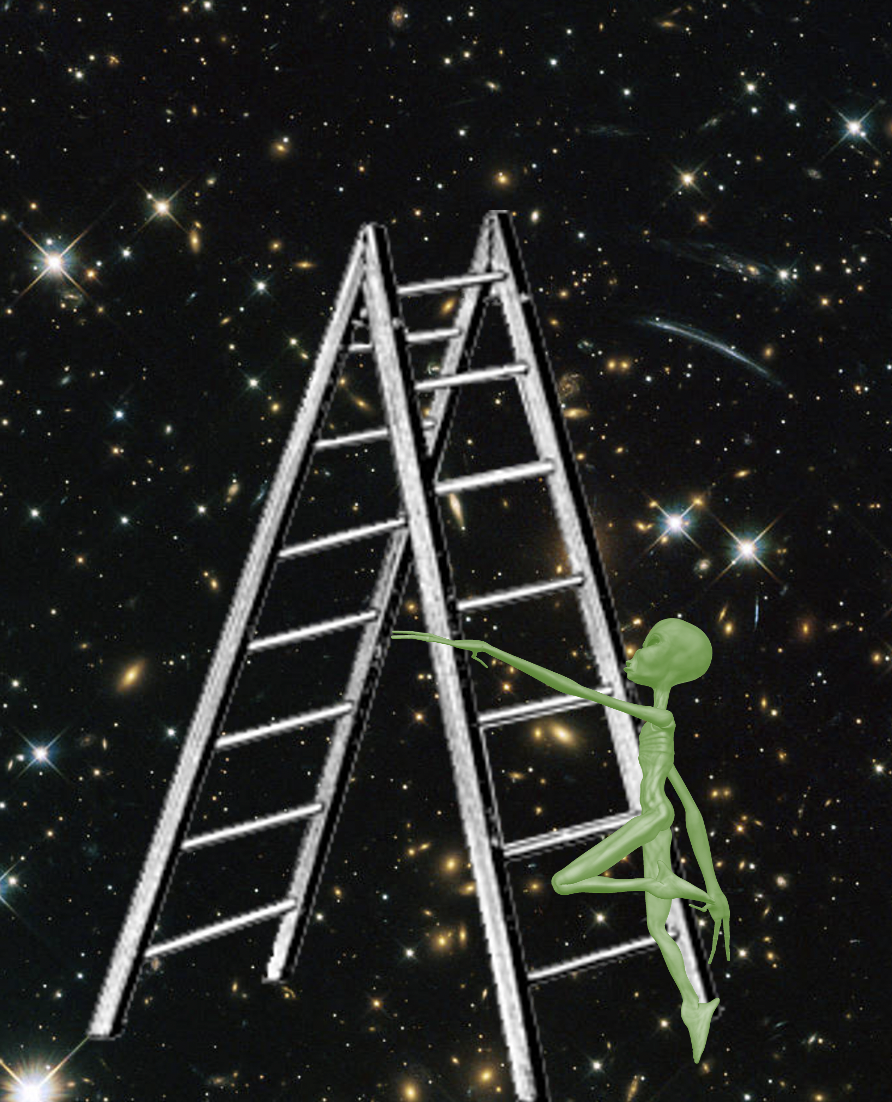
\includegraphics[scale=0.4]{media/ladder1.png}
\column{0.5\textwidth}
{\small
\textcolor{yellow}{Velkommen til del 3A! I denne delen av kurset skal vi se hvordan vi kan finne avstander til objekter i verdensrommet. Det finnes mange forskjellige metoder, noen egner seg for det nære verdensrom, andre kun for veldig fjerne objekter. Ofte bygger de på hverandre slik at metodene for fjernere objekter må kalibereres med metodene for nære objekter, og slik må man gå steg for steg med metode for metode lenger og lenger utover i universet. Derfor kalles spektret av metoder for avstandsmålinger for {\bf den kosmiske avstandsstigen}.}\textcolor{blue}{\bf\footnotesize (illustrasjon: Credit: ESA/Hubble \& NASA, RELICS; Acknowledgement: D. Coe et al. + Hiclipart)}\hyperlink{intro2}{\pagebutton{Neste side}}
}
\end{columns}
\end{frame}
}


\begin{frame}
\label{intro2}
\lastpagebutton{feil_intro}
Dette interaktive forelesningsnotatet tilsvarer omkring en og en halv dobbelttime forelesning. Du får beskjed når du har kommet til det punktet jeg pleier å komme til i den første forelesningen (avsnittet om avstandsindikatorer).
\begin{alertblock}{Vi begynner som vanlig...}
...med litt brainstorming. Som det er {\bf svært viktig} at du gjør før du går videre.
\end{alertblock}
\href{https://nettskjema.no/a/165578}{\begin{minipage}{5cm}Trykk her for å varme opp\end{minipage}}\\
Er du klar og har sendt inn skjemaet?
\href{https://nettskjema.no/a/165578}{\choicebutton{Nei}}\ \ \ \ \hyperlink{feil_nytema1}{\choicebutton{Ja}}\\
%\hyperlink{intro2}{\choicebutton{Nei}}\ \ \ \ \hyperlink{brainstormdone}{\choicebutton{Ja}}\\
\end{frame}

\renewcommand{\headline}{\small parallakse}
{
\setbeamercolor{background canvas}{bg=black}
\begin{frame}
\label{feil_nytema1}
\begin{columns}
\column{0.5\textwidth}
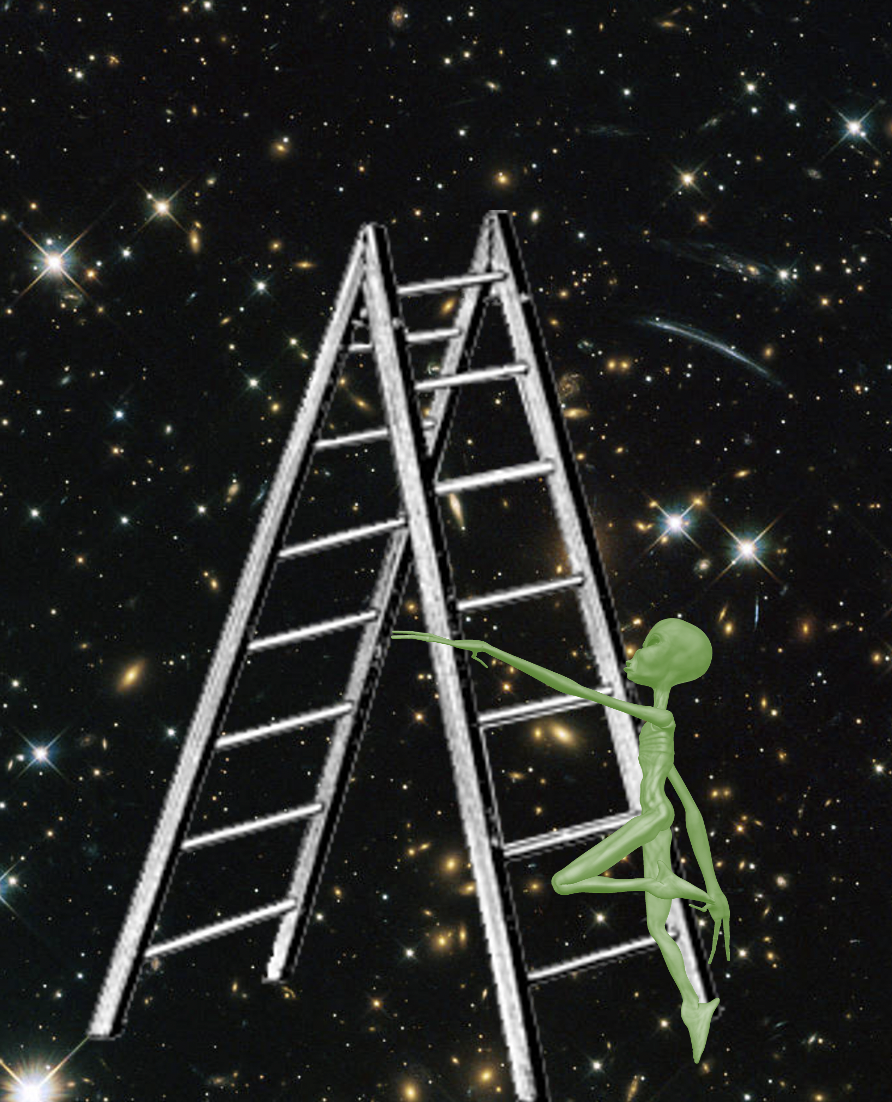
\includegraphics[scale=0.4]{media/ladder1.png}
\hyperlink{intro2}{\pagebutton{\small Forrige side}}
\column{0.5\textwidth}
\textcolor{red}{\small Vi begynner med det første steget på avstandsstigen:}\vspace*{1cm}
\nytemaside{hrfit}
\hyperlink{paral1}{\pagebutton{La oss begynne å klatre!}}
\end{columns}
\end{frame}
}


\begin{frame}
\label{paral1}
\dlastpagebutton{intro2}
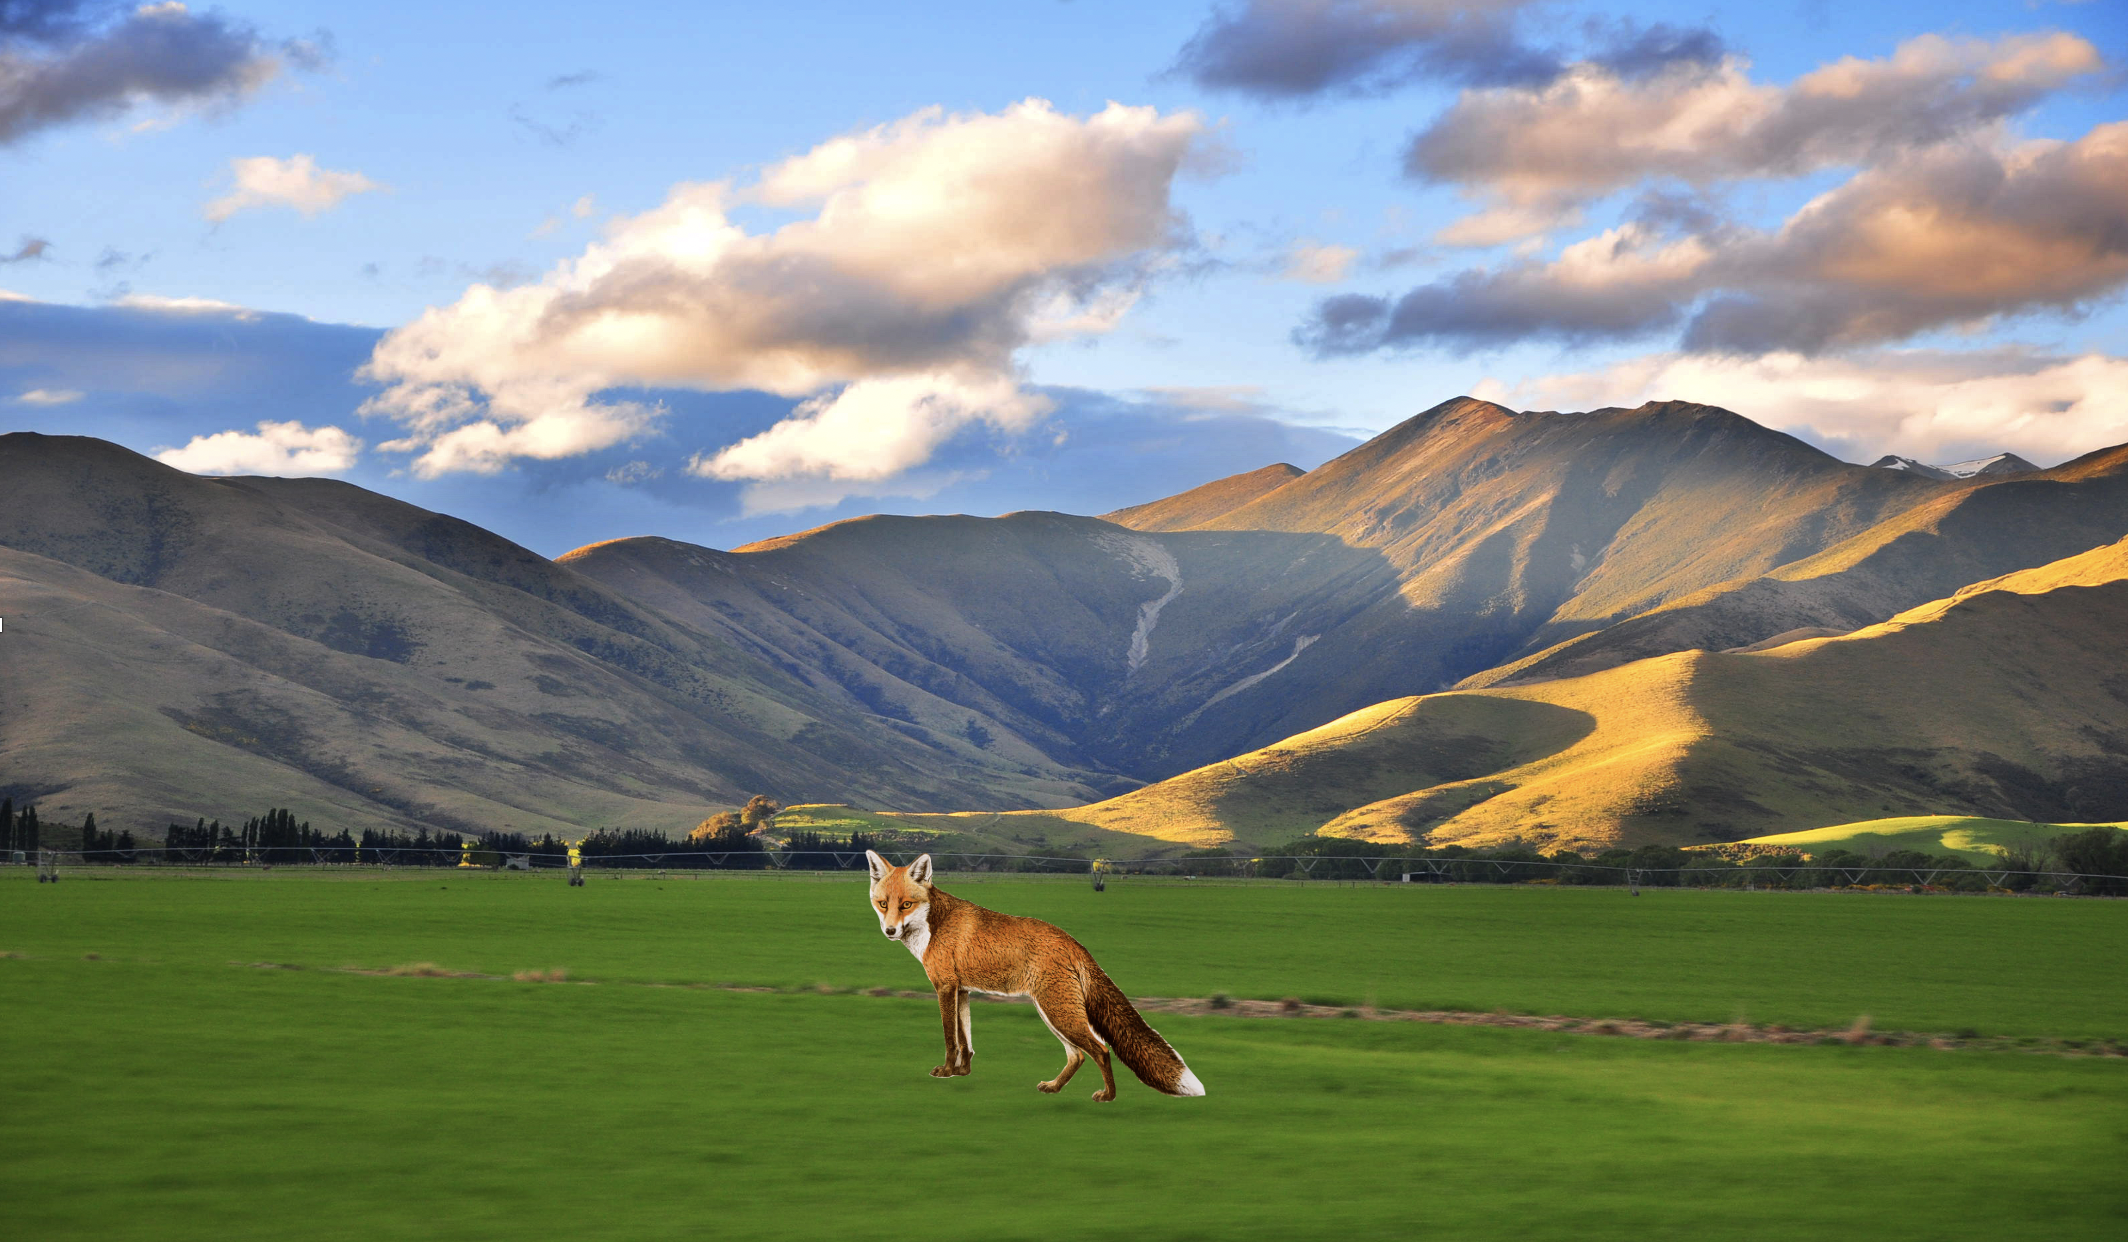
\includegraphics[scale=0.3]{media/fox_middle.png}\hspace*{-11.3cm}{\tiny\textcolor{white}{Bilde fra:https://all-free-download.com/free-photos/download/nz-landscape-from-the-van\_514273.html, author: Benurs}}\\
{\footnotesize Du kikker utover et fjell-landskap. I det fjerne kan du se fjell, men plutselig ser du en rev rett foran deg! Hvis du nå {\bf lukker det høyre øyet ditt}, tror du at dette kommer til å se forskjellige ut på noen måte? {\bf Hva tror du endrer seg?} } \textcolor{red}{\footnotesize MERK: siden dette er en 2D-skjerm vil du ikke se effekten her, du må tenkte deg hva som ville skjedd hvis du virkelig stod der ute på fjellet!}\hyperlink{paral2}{\pagebutton{\footnotesize Tenk deg godt om før du blar om!}}
\end{frame}

\begin{frame}
\label{paral2}
\lastpagebutton{paral1}
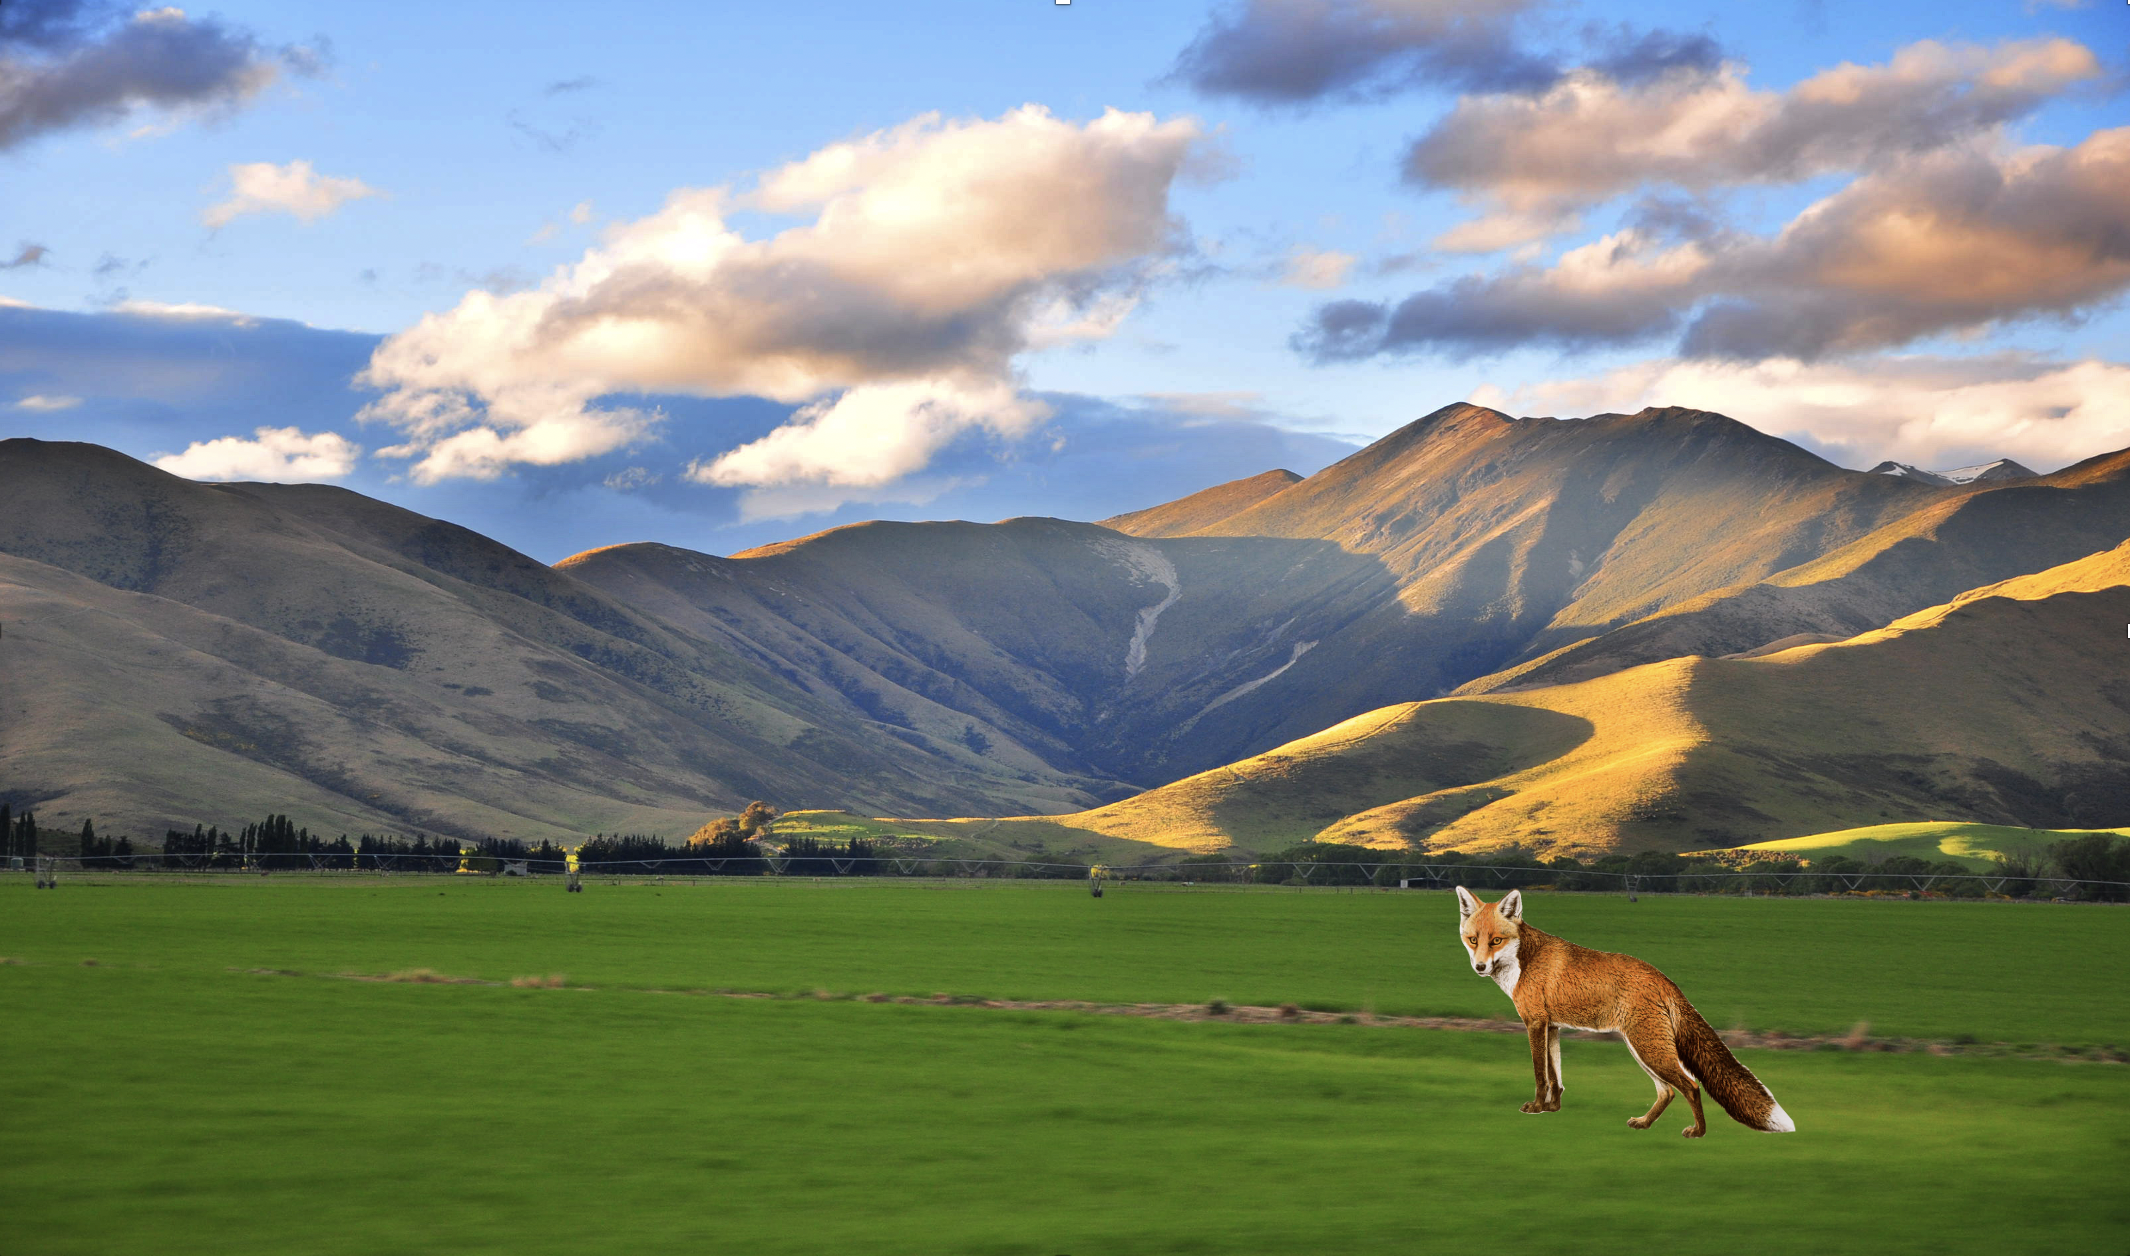
\includegraphics[scale=0.3]{media/fox_right.png}\hspace*{-11.3cm}{\tiny\textcolor{white}{Små figurer: fra hiclipart.com}}\\
{\bf Ser du forskjellen?} Bla gjerne litt frem og tilbake mellom denne og forrige side for å se om du ser forskjellen! {\bf Hva skjedde? Hvorfor ble det slik?}
\hyperlink{red_paral3}{\pagebutton{Tenk deg godt om før du blar om!}}
\end{frame}


{
\setbeamercolor{background canvas}{bg=red}
\begin{frame}
\label{red_paral3}
\lastpagebutton{paral2}
\textcolor{yellow}{\Large Fant du ut av det??}
\textcolor{yellow}{Hvis ikke, prøv å tegne alt ovenfra: begge øynene dine, reven og fjellene. Ser du det nå?}
\hyperlink{paral4}{\pagebutton{Tenk deg godt om før du blar om!}}
\end{frame}
}


\begin{frame}
\label{paral4}
\lastpagebutton{red_paral3}
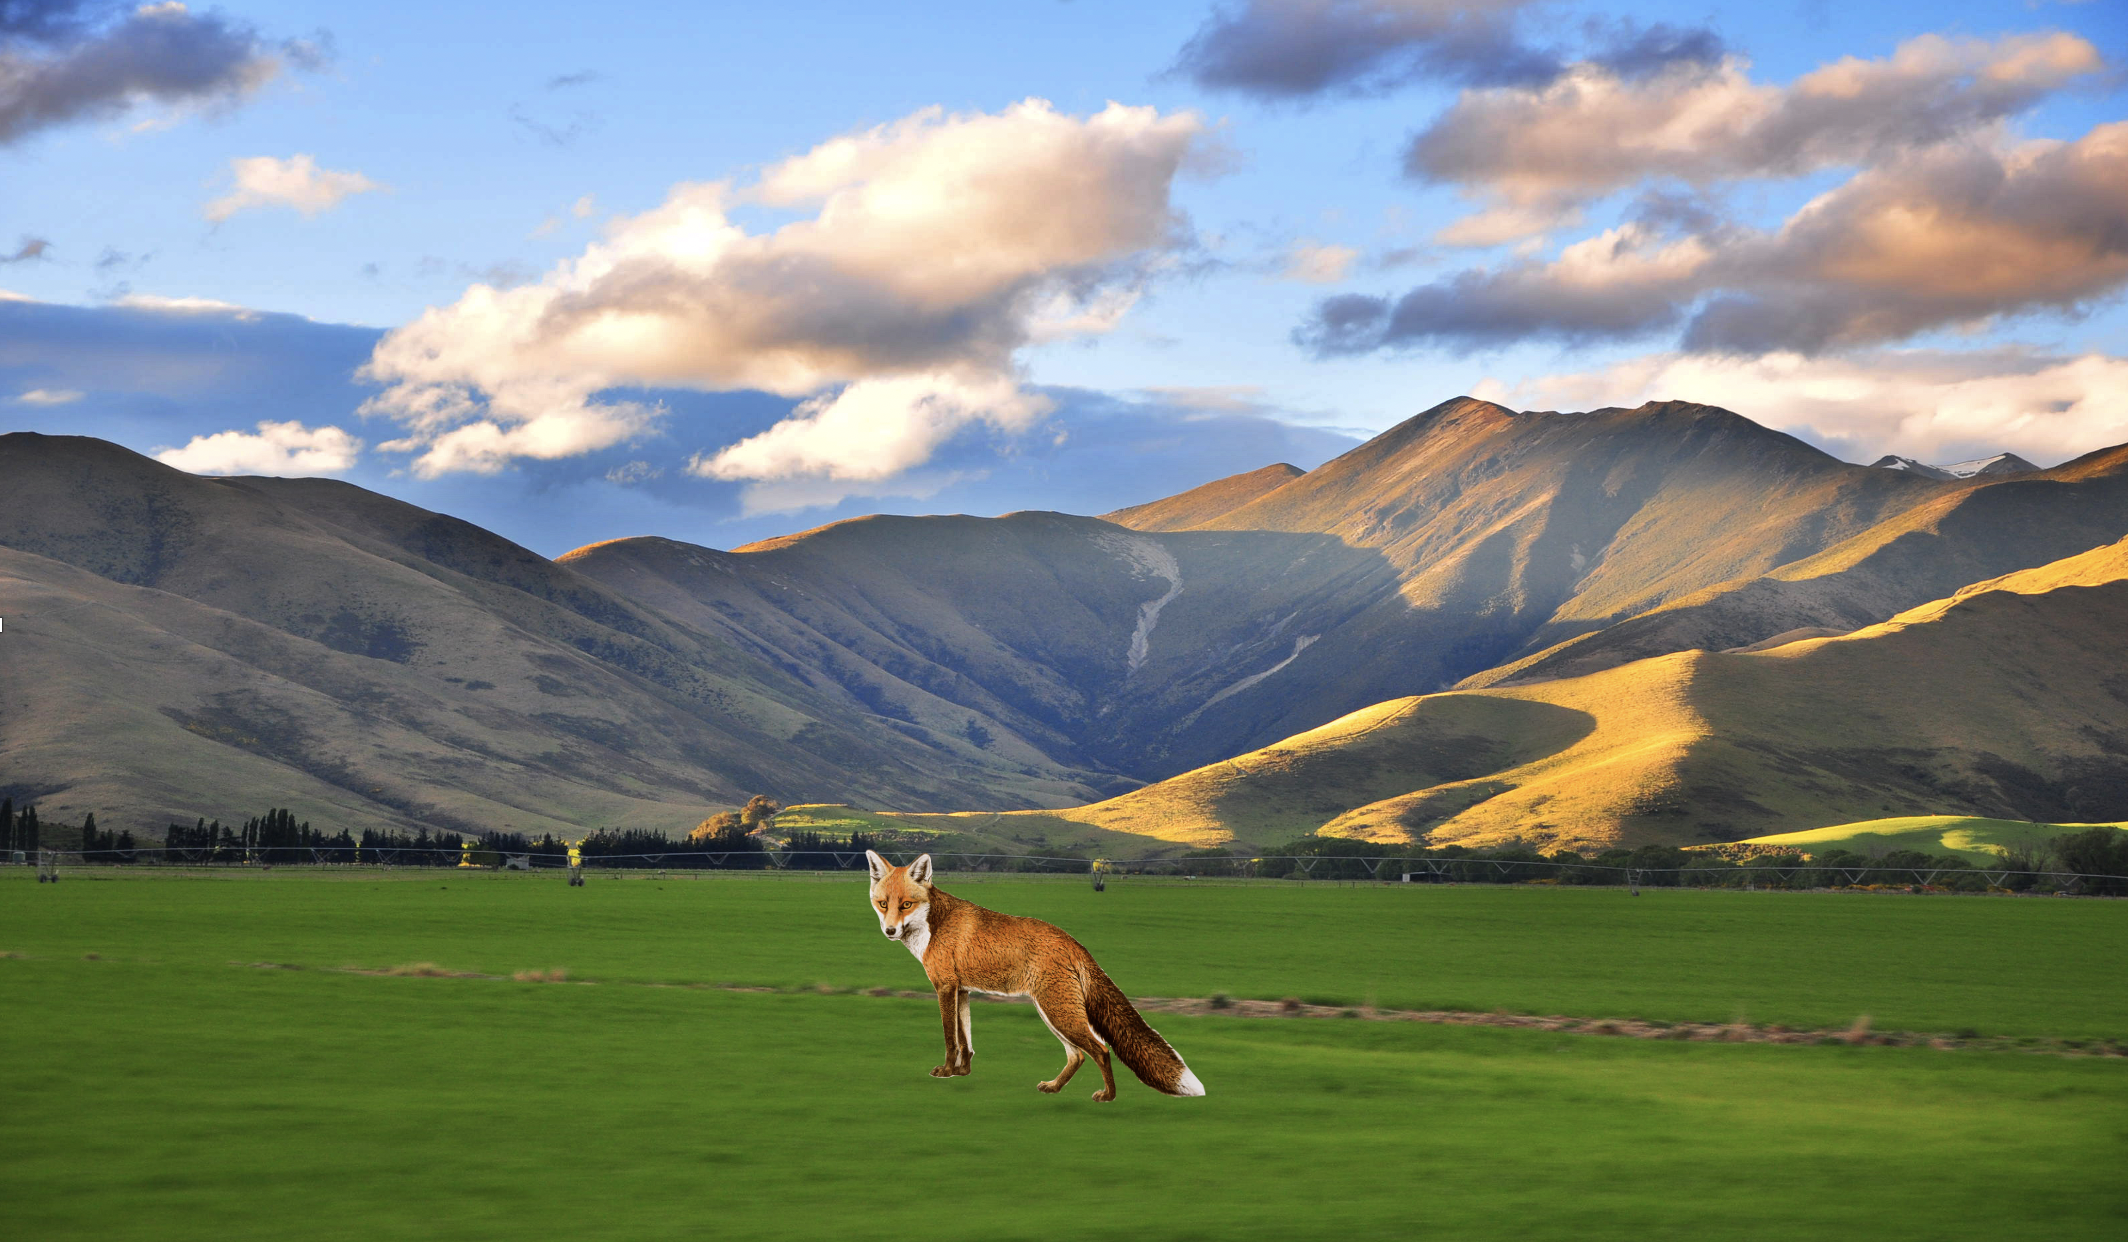
\includegraphics[scale=0.3]{media/fox_middle.png}\\
{\footnotesize Hvis du nå har en teori, la oss se om du tar denne testen først: Her ser vi situasjonen med begge øyne igjen. Hvis du nå isteden lukker {\bf det venstre} øyet ditt, {\bf hva tror du da skjer?} \textcolor{red}{ Hi, hi, tenker du nok, {\bf det er jo opplagt}, men nå blir du lurt, så sjekk tegningen din fra forrige side skikkelig før du} \hyperlink{paral5}{\pagebutton{\footnotesize blar om.}}}
\end{frame}



\begin{frame}
\label{paral5}
\lastpagebutton{paral4}
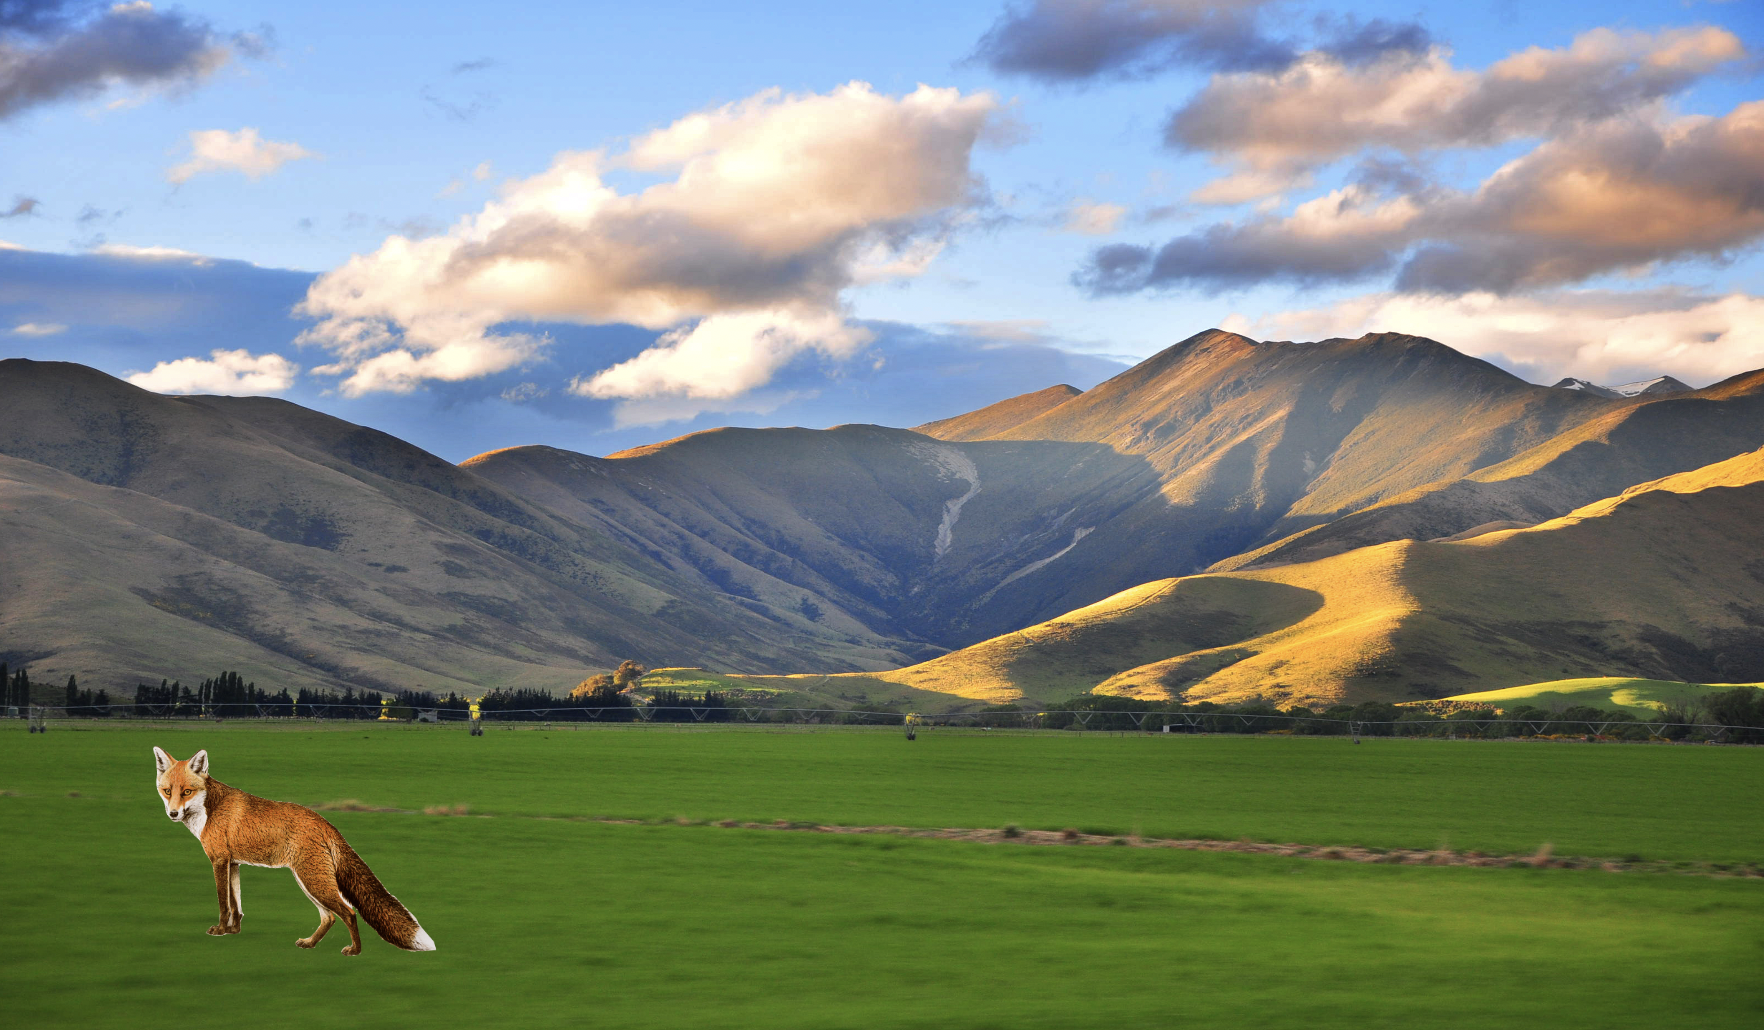
\includegraphics[scale=0.36]{media/fox_left.png}\\
{\bf Ok da,} du ble ikke lurt (dvs. du ble lurt til å tro at du ble lurt...). Reven ser du plutselig nå til venstre. {\bf Men hva er det som skjer?}
\hyperlink{paral6}{\pagebutton{Tenk deg godt om før du blar om!}}
\end{frame}

\begin{frame}
\label{paral6}
\lastpagebutton{paral5}
\centerline{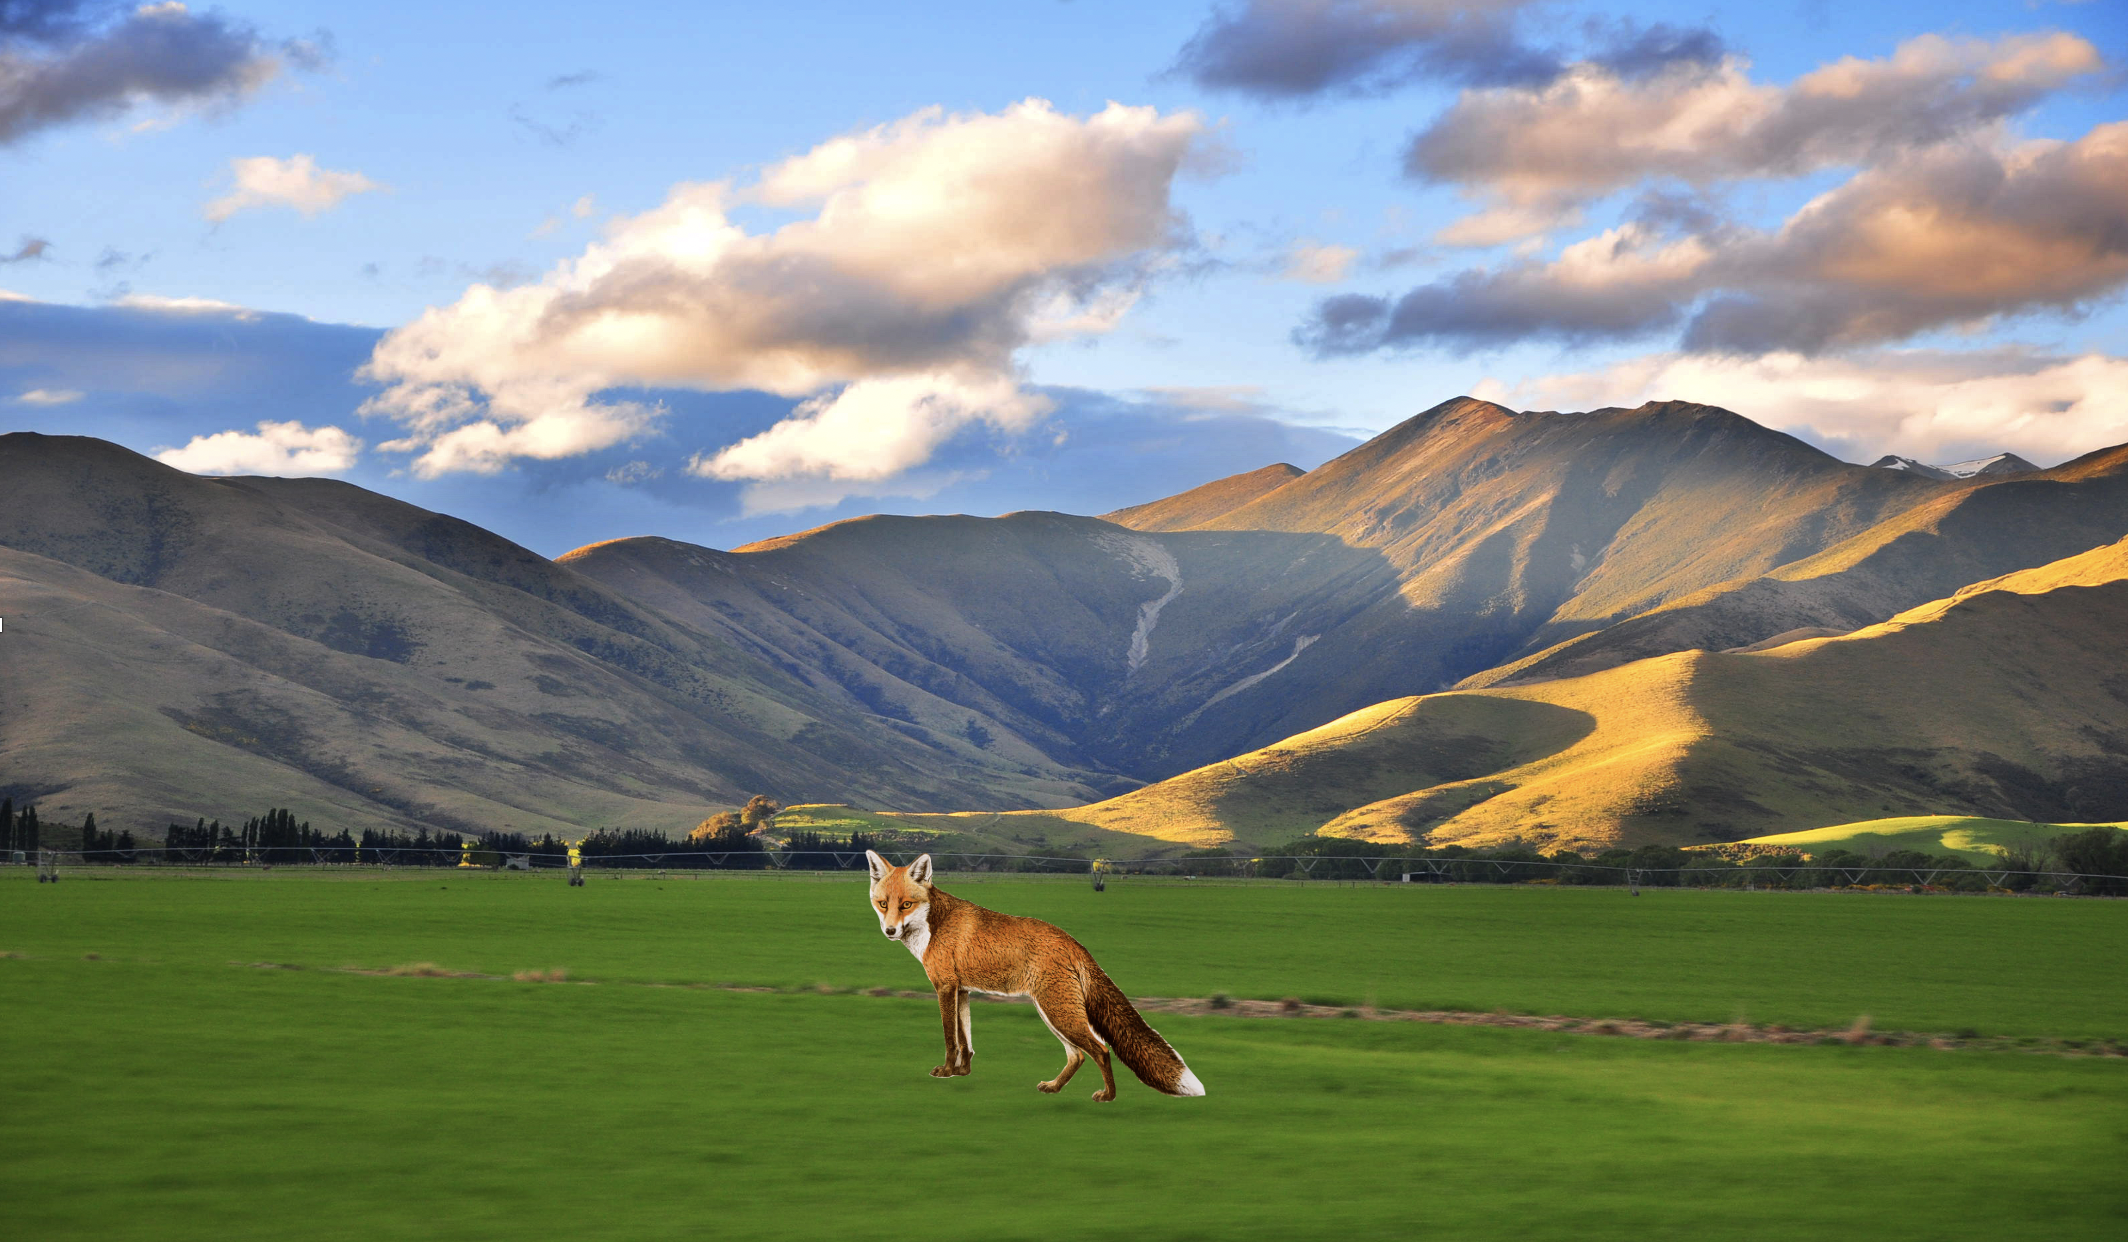
\includegraphics[scale=0.2]{media/fox_middle.png}}
{\footnotesize Ja, hvis du ikke ser det, så skal jeg holde deg på pinebenken litt til. Nå skal du få en praktisk øvelse: hold tommelen opp foran ansiktet ditt (omtrent i midten). Se på tommelen med begge øyne. Lukk det ene øyet og se hvor tommelen er i forhold til et eller annet langt borte i bakgrunnen. Så lukker du isteden det andre øyet og ser hvor tommelen er i forhold til den samme tingen. {\bf Flytter den seg på samme måte som reven? Hvorfor?}}
\hyperlink{paral7}{\pagebutton{Tenk deg godt om før du blar om!}}
\end{frame}

\begin{frame}
\label{paral7}
\lastpagebutton{paral6}
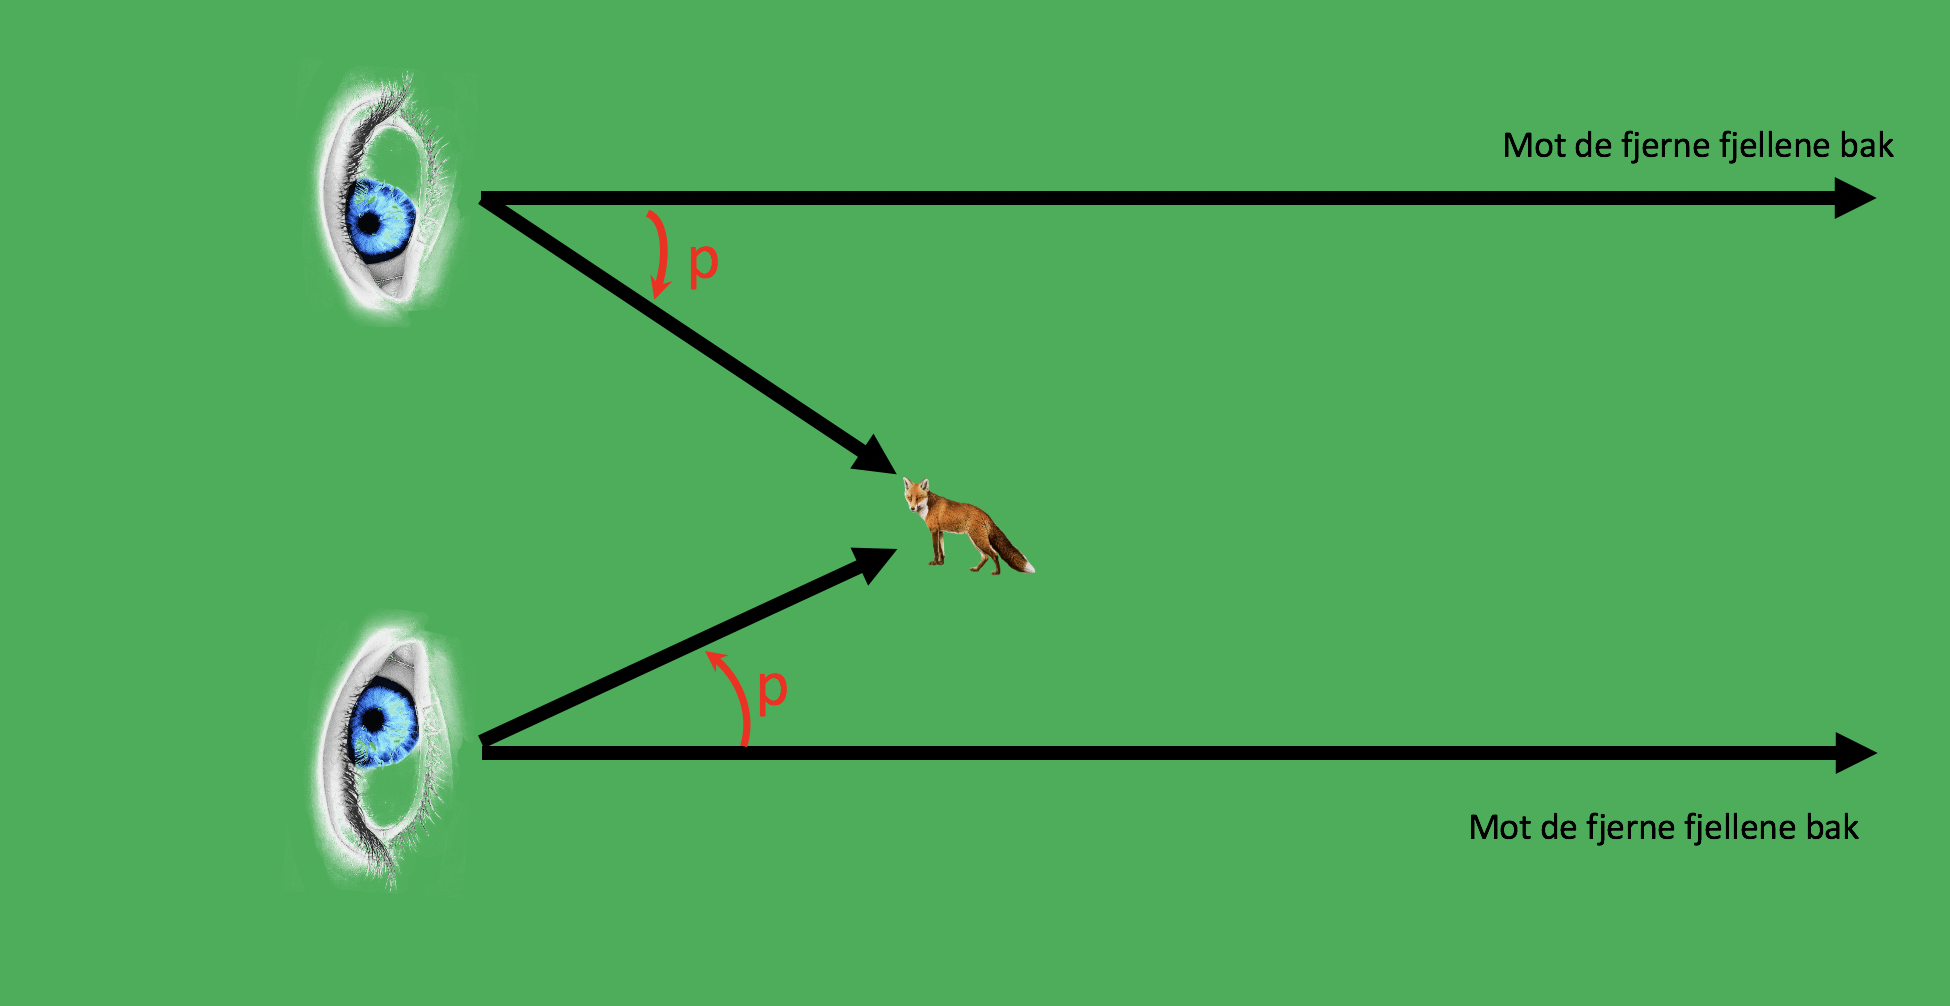
\includegraphics[scale=0.3]{media/fox_eyes.png}\hspace*{-9cm}{\tiny\textcolor{white}{Små figurer: fra hiclipart.com}}\\
Her ser du situasjonen ovenfra. Merk at siden fjellene er veldig langt borte så vil linjene fra hver av øynene til fjellene være nesten parallelle (har du lagt merke til at hvis du kjører bil og har månen rett over deg, så vil månen enda være rett over deg etter at du har kjørt en god stund. Linja fra deg til månen er rett opp i begge tilfeller). {\bf Ser du at fra det ene øyet er reven en vinkel $p$ til venstre for fjellet, fra det andre øyet er reven en vinkel $p$ til høyre?}
\hyperlink{paral8}{\pagebutton{Ja, ser det nå!}}
\end{frame}

\begin{frame}
\label{paral8}
\lastpagebutton{paral7}
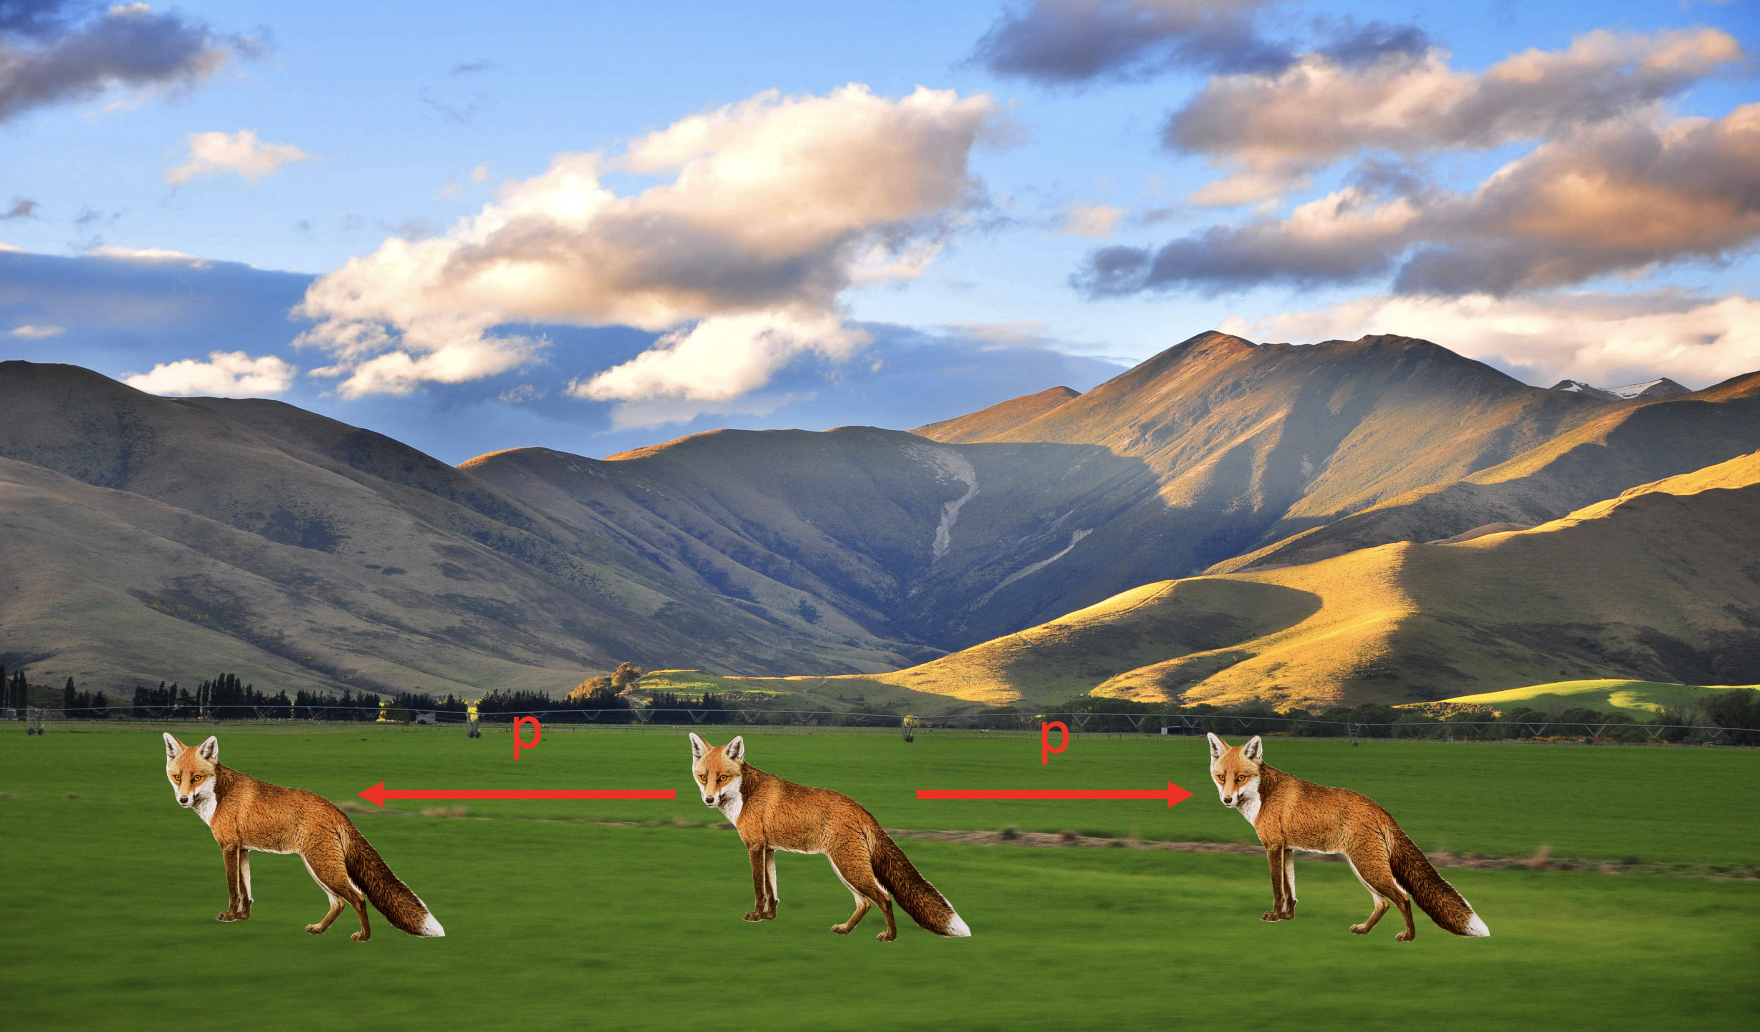
\includegraphics[scale=0.36]{media/all_foxes.png}\\
{\small Ser du at reven har flyttet seg en vinkel $2p$ fra det ene øyet til det andre? Hvis du peker på reven i det ene tilfellet og så flytter armen til å peke på reven i det andre tilfellet, vil du ha beveget armen en vinkel $2p$. Vi kaller $p$ {\bf parallaksevinkelen}. \textcolor{red}{ Men stopp en hal, er vinkelen $p$ her den samme som på forrige figur??}}
\hyperlink{paral8b}{\pagebutton{Tjaaaaa}}
\end{frame}

\begin{frame}
\label{paral8b}
\lastpagebutton{paral8}
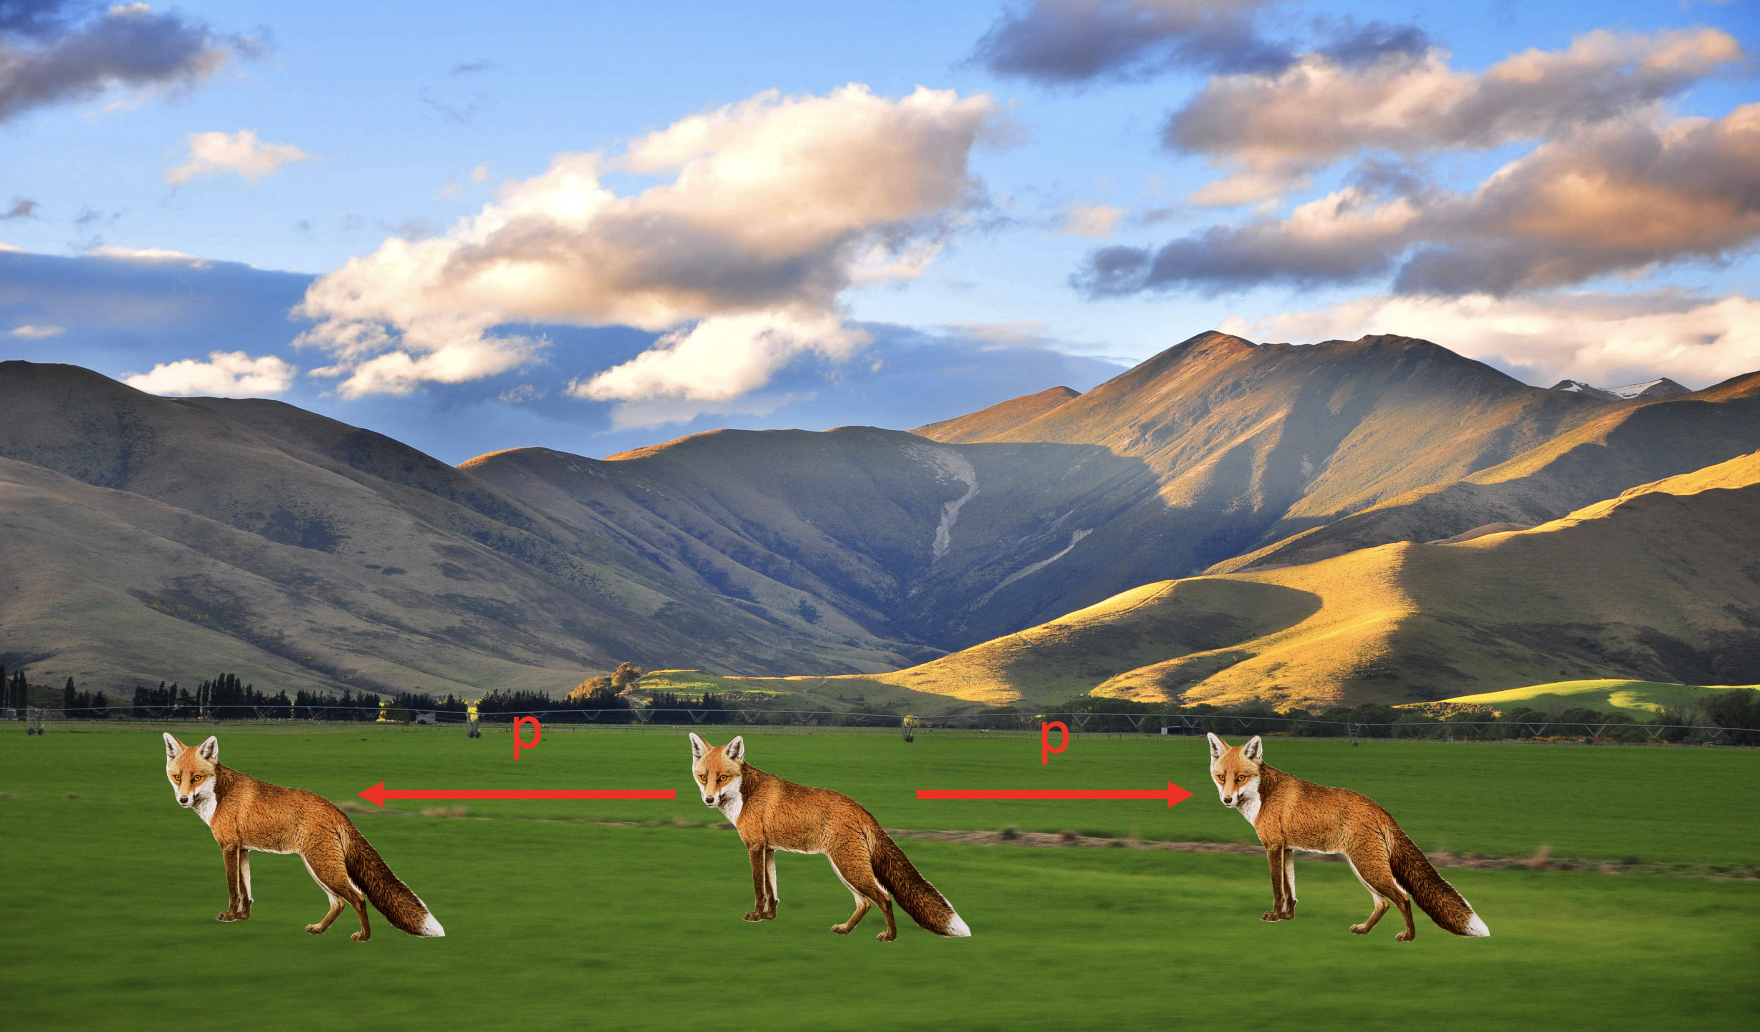
\includegraphics[scale=0.19]{media/all_foxes.png}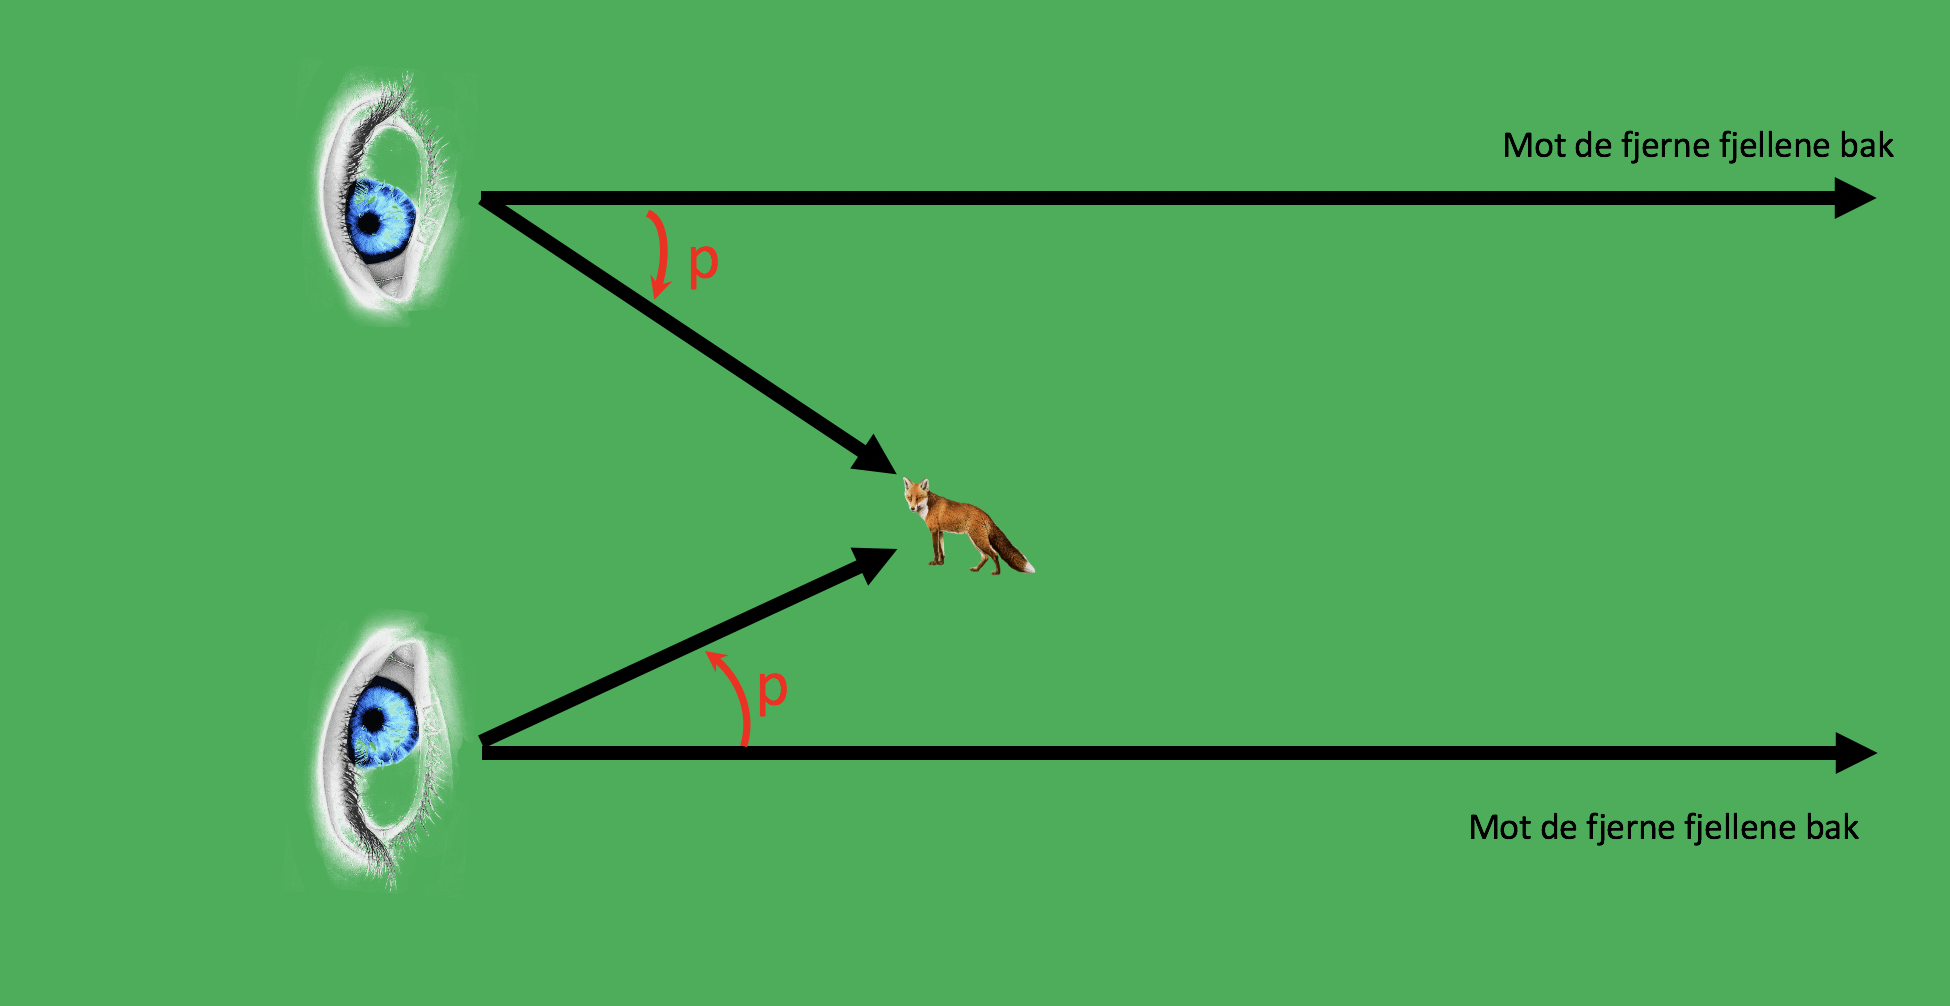
\includegraphics[scale=0.19]{media/fox_eyes.png}\\
{\bf Ser du det??} Hvis ikke, spør! Men hva tror du vinkelen $p$ avhenger av? Hvordan kunne du fått denne vinkelen til å bli større eller mindre? Kanskje du kan prøve deg frem med tommelen og se om du ser det?
\hyperlink{paral9}{\pagebutton{Neste side}}
\end{frame}

\begin{frame}
\label{paral9}
\lastpagebutton{paral8b}
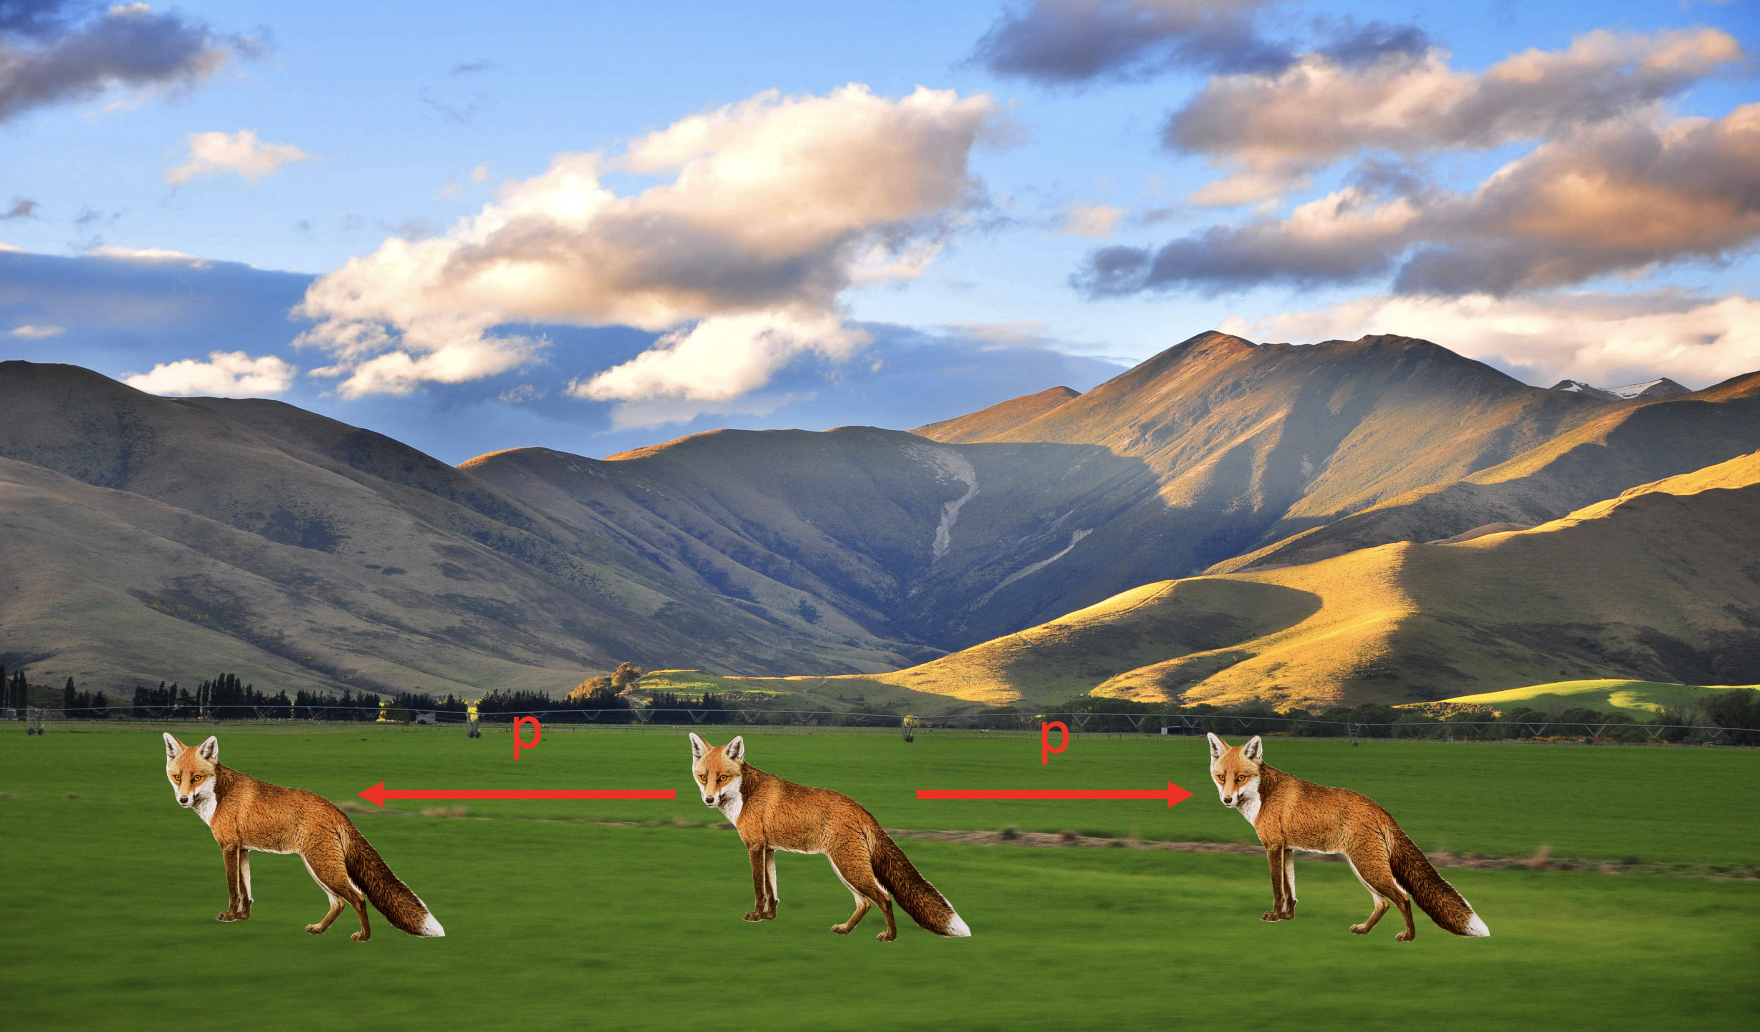
\includegraphics[scale=0.19]{media/all_foxes.png}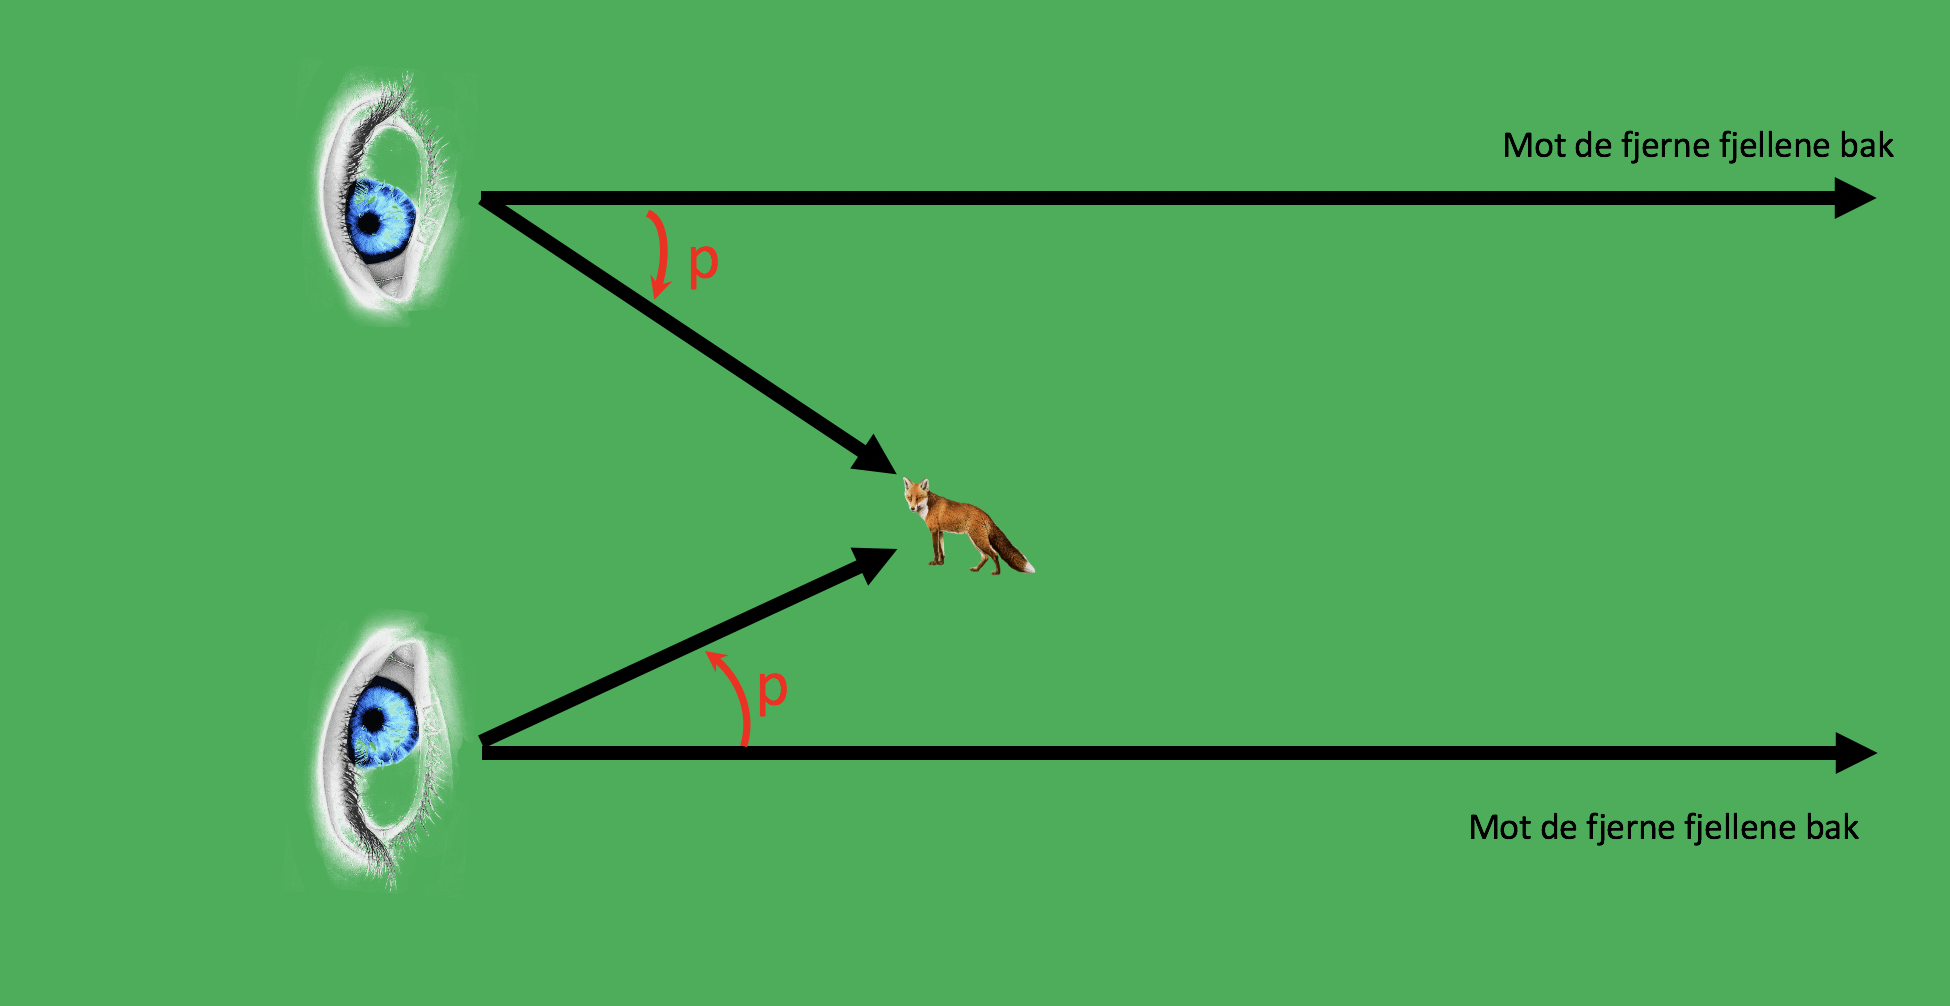
\includegraphics[scale=0.19]{media/fox_eyes.png}\\
Hva vil skje med vinkelen $p$ hvis reven kommer lenger og lenger bort, og etterhvert nærmer seg fjellene?
\hyperlink{paral10}{\pagebutton{Nå tror jeg at jeg ser det!}}
\end{frame}

\begin{frame}
\label{paral10}
\lastpagebutton{paral9}
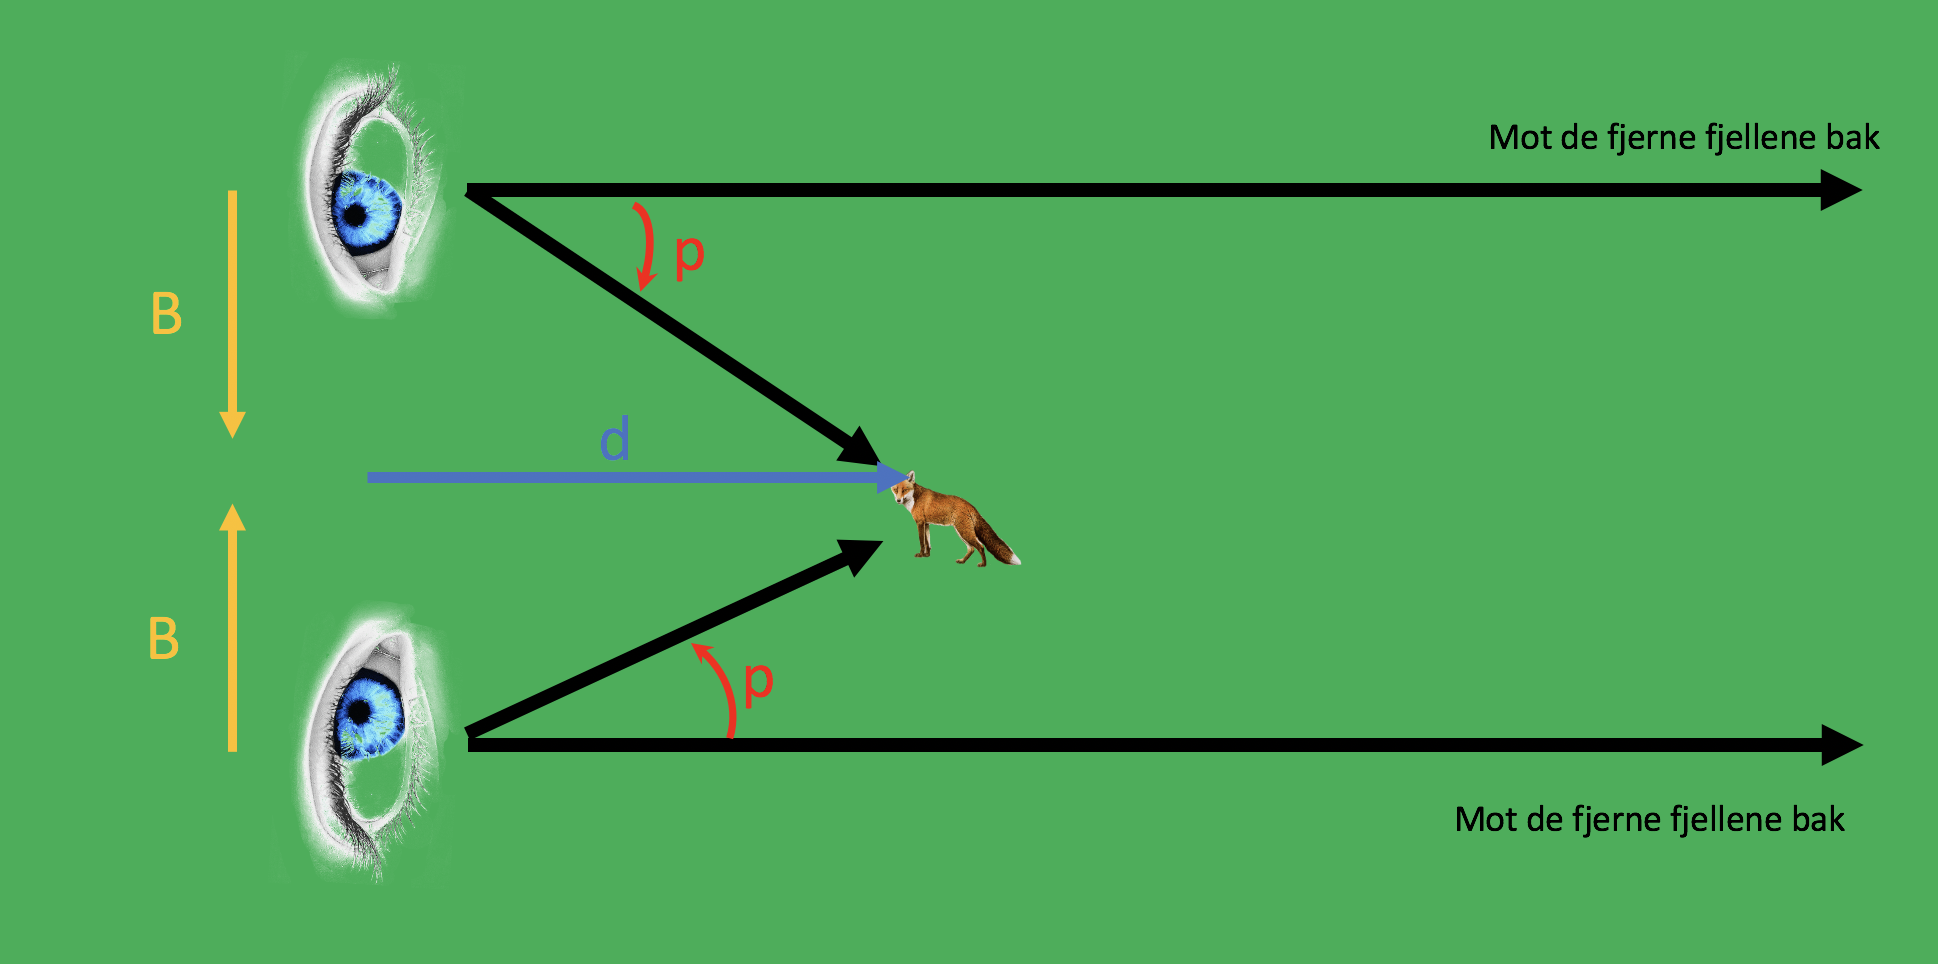
\includegraphics[scale=0.36]{media/fox_eyes_distance.png}\\
Her er $B$ avstand fra nese til øye, vi kaller det {\bf baseline} på engelsk, og $d$ er avstanden til reven. Kan du finne en sammenheng mellom disse 3 størrelsene? {\bf Hint:} du kan anta at parallaksevinkelen er liten, det er den nesten alltid i sammenhenger der parallakse brukes.
\hyperlink{paral11}{\pagebutton{\small Jeg har kommet frem til en formel, eller ihvertfall prøvd hardt!}}
\end{frame}

\begin{frame}
\label{paral11}
\lastpagebutton{paral10}
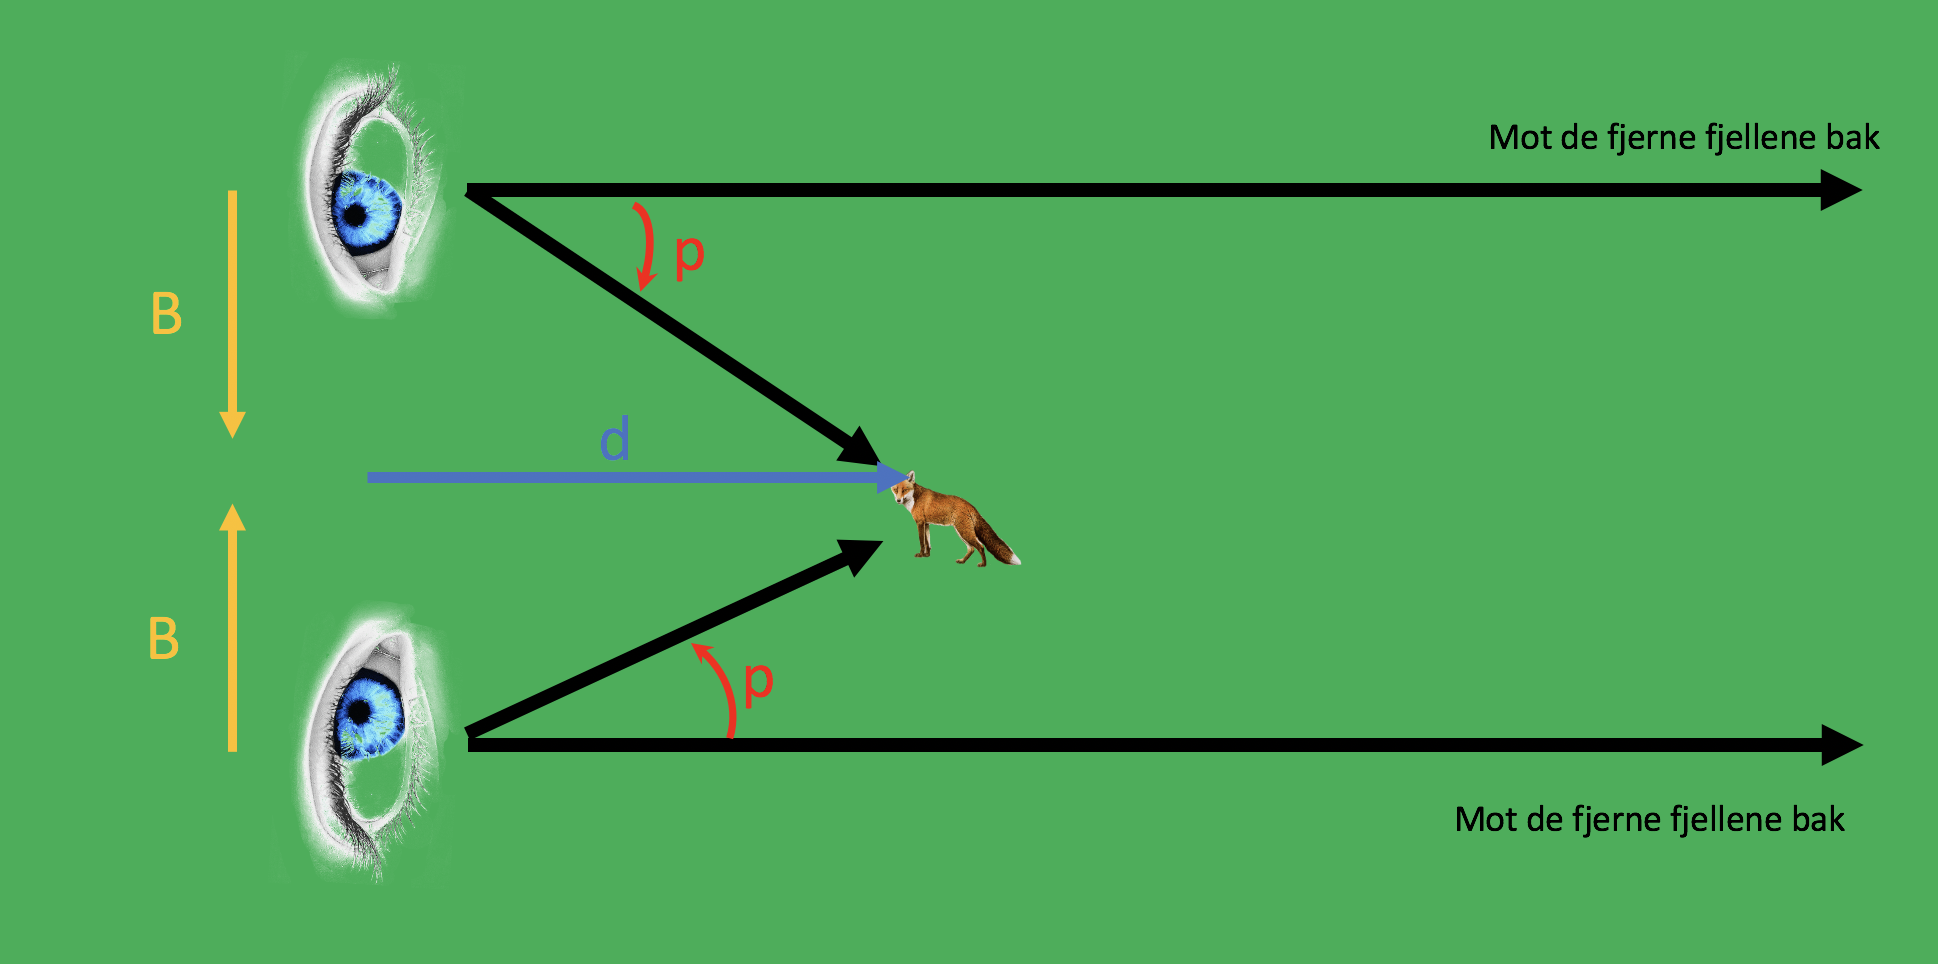
\includegraphics[scale=0.36]{media/fox_eyes_distance.png}\\
Husker du liten-vinkel-formelen? Den bør du kunne utlede selv uten hjelp. Hvis du ikke allerede har et svar, prøv igjen nå med liten-vinkel-formel...
\hyperlink{paral12}{\pagebutton{\small Nå ser jeg det!}}
\end{frame}

\begin{frame}
\label{paral12}
\lastpagebutton{paral11}
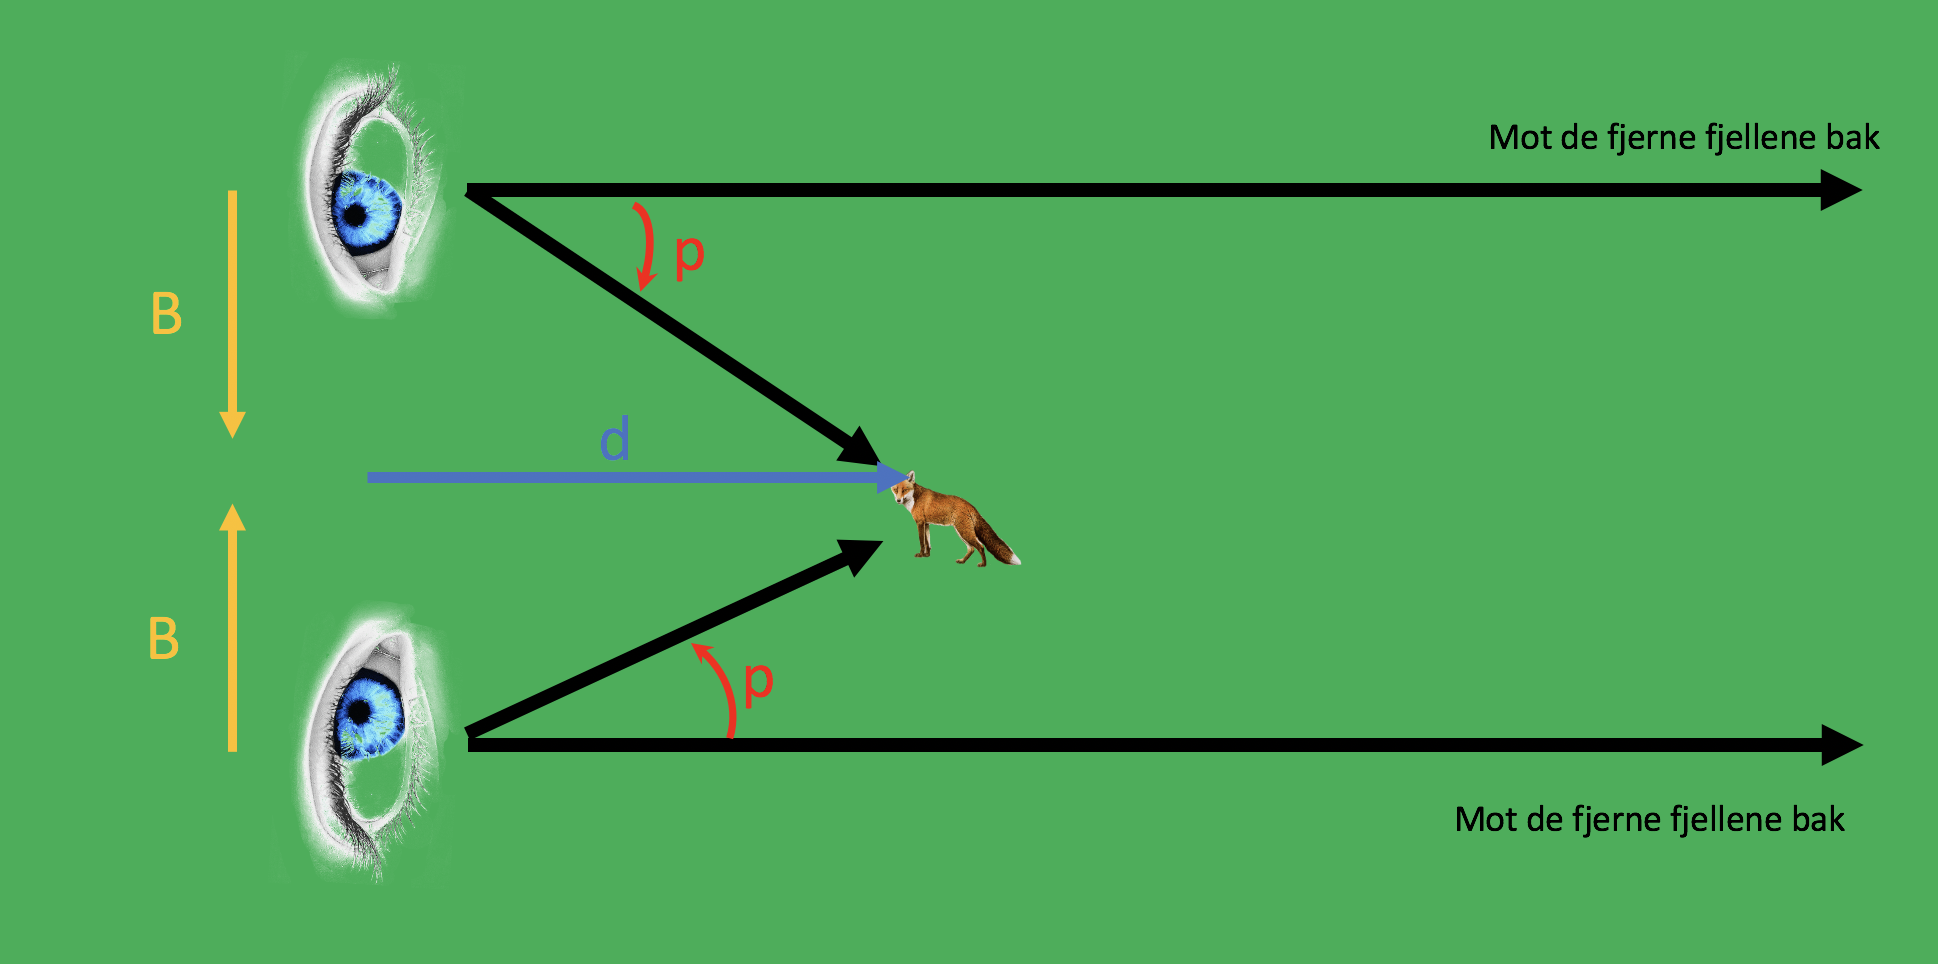
\includegraphics[scale=0.36]{media/fox_eyes_distance.png}\\
Liten-vinkel-formel gir:
\[
B=dp\ \ \ \textrm{(hvor\ p\ må\ være\ i\ radianer)}
\]
\textcolor{red}{Hvis vi sier at avstanden mellom nese og øye er 10cm, og du ser en endring i revens posisjon på 0.1 grad fra et øye til det andre, hvor langt unna er revet?}
\hyperlink{paral13}{\pagebutton{\small Jeg har et svar!}}
\end{frame}

\begin{frame}
\label{paral13}
\lastpagebutton{paral12}
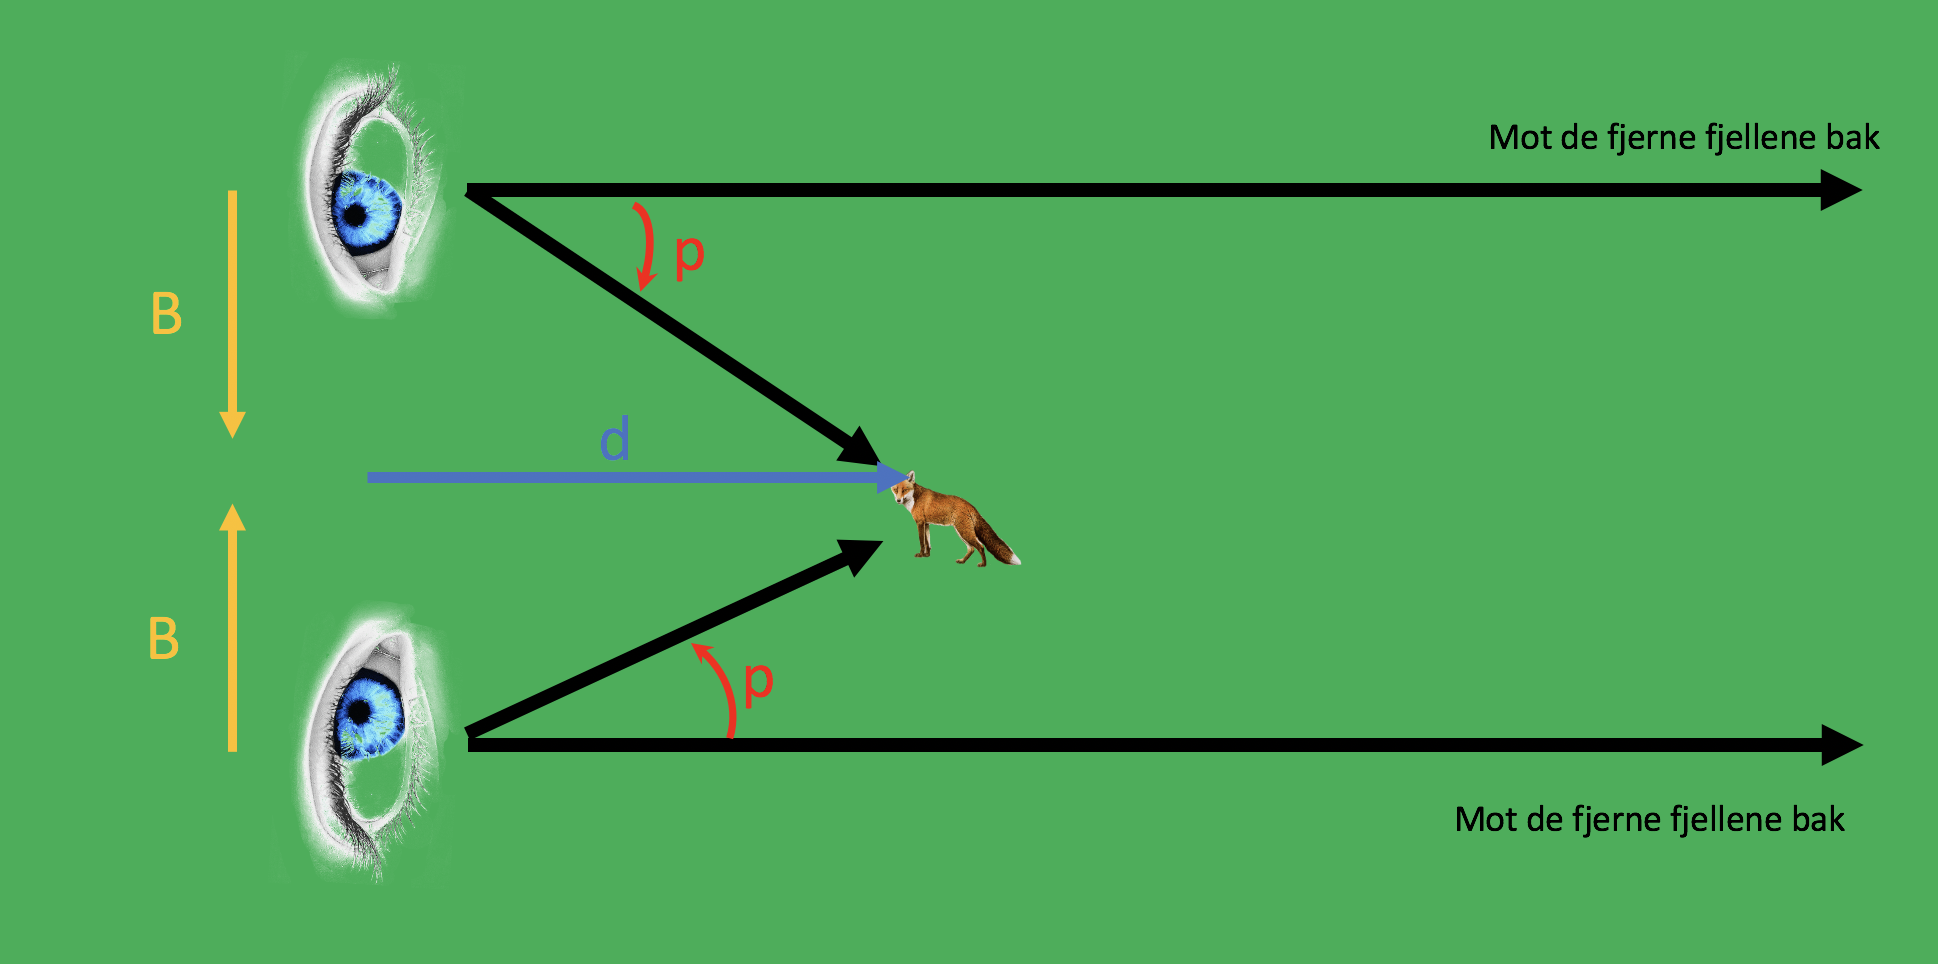
\includegraphics[scale=0.36]{media/fox_eyes_distance.png}\\
Er avstanden til reven:\hyperlink{feil_paral13a}{\choicebutton{229m}}\ \ \ \hyperlink{feil_paral13a}{\choicebutton{57m}}\ \ \ \ \hyperlink{feil_paral13a}{\choicebutton{286m}}\ \ \ \ \hyperlink{riktig_paral13b}{\choicebutton{115m}}
\end{frame}

{
\setbeamercolor{background canvas}{bg=black}
\begin{frame}
\label{feil_paral13a}
\lastpagebutton{paral13}
\centerline{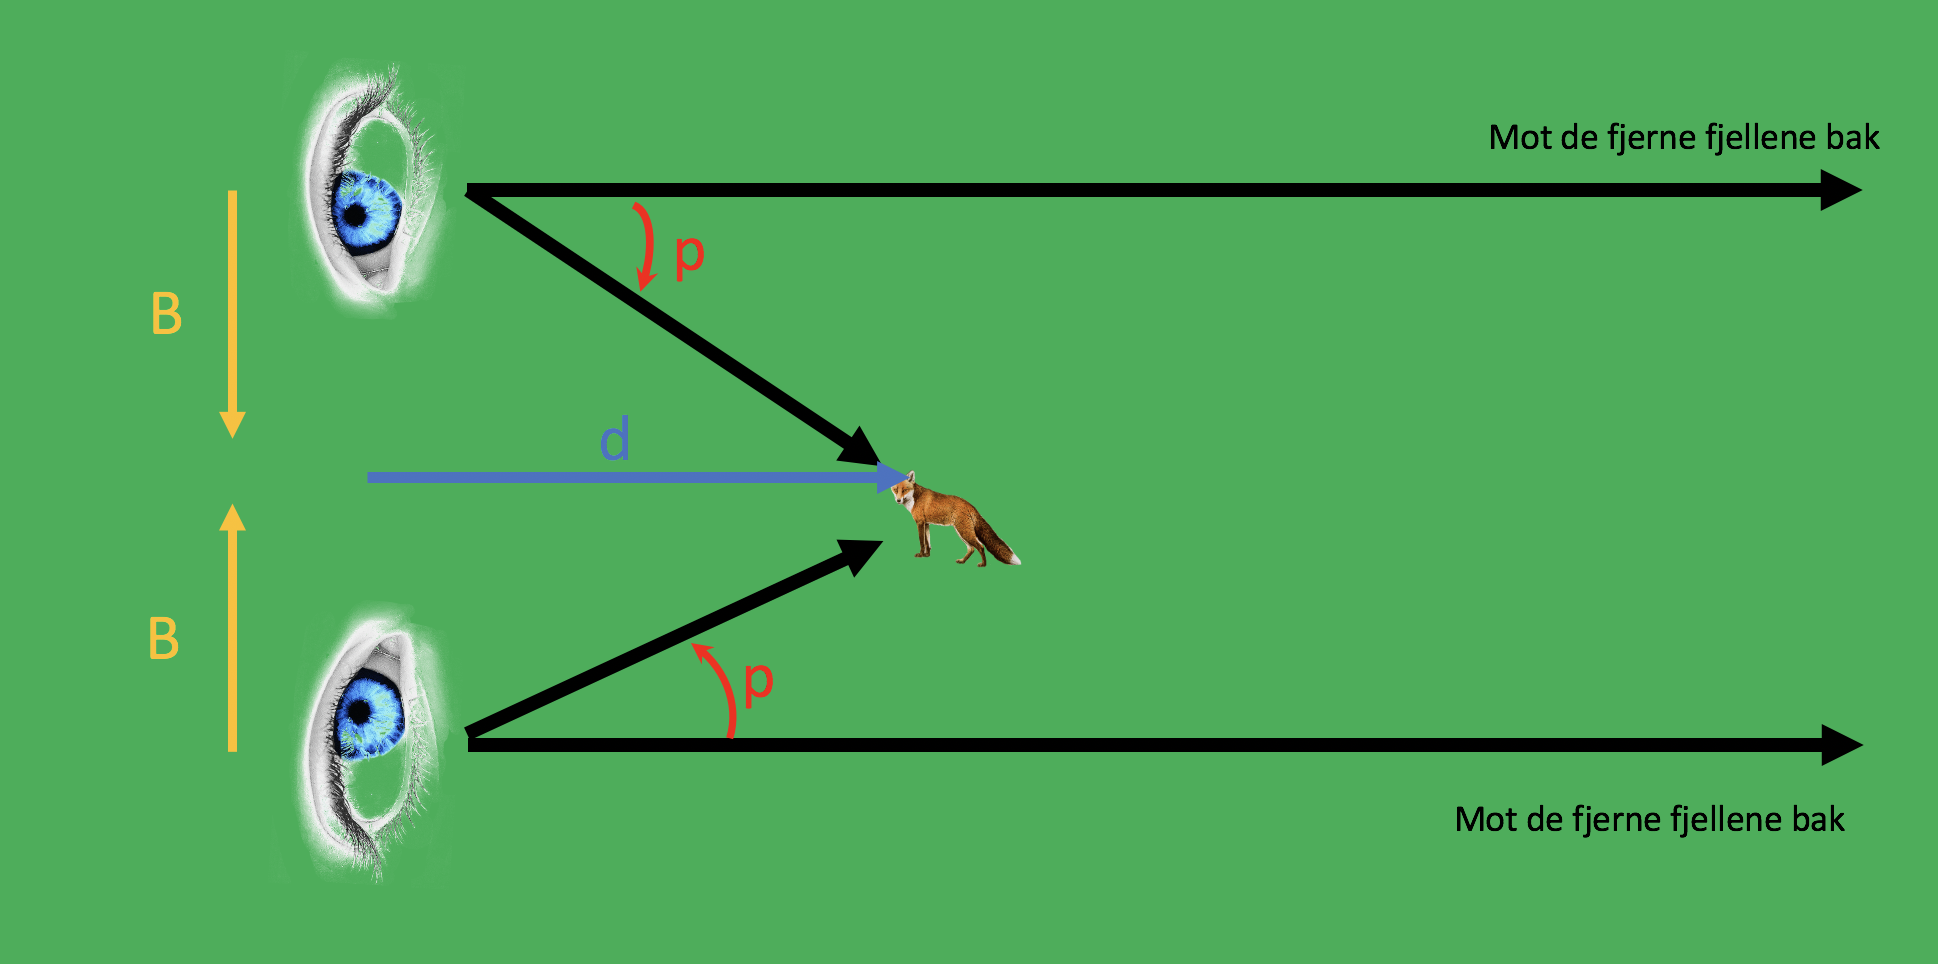
\includegraphics[scale=0.3]{media/fox_eyes_distance.png}}
\textcolor{yellow}{\Large Det ble galt! Ble du kanskje lurte av en faktor 2 her? Husk at {\bf $B$ er avstanden fra nese til øye}, $2B$ er avstand fra øye til øye. Og {\bf parallaksevinkelen $p$ er definert som vinkelen fra to øyer (altså midten) til et øye} mens $2p$ er vinkelen fra øye til øye! Ser du det på figuren? Dette er en veldig typisk feil på eksamen, veldig bra at du gjorde den her og ikke på eksamen. Nå gjør du ikke denne feilen igjen!}
\end{frame}
}

{
\setbeamercolor{background canvas}{bg=yellow}
\begin{frame}
\label{riktig_paral13b}
\clastpagebutton{paral13}
\centerline{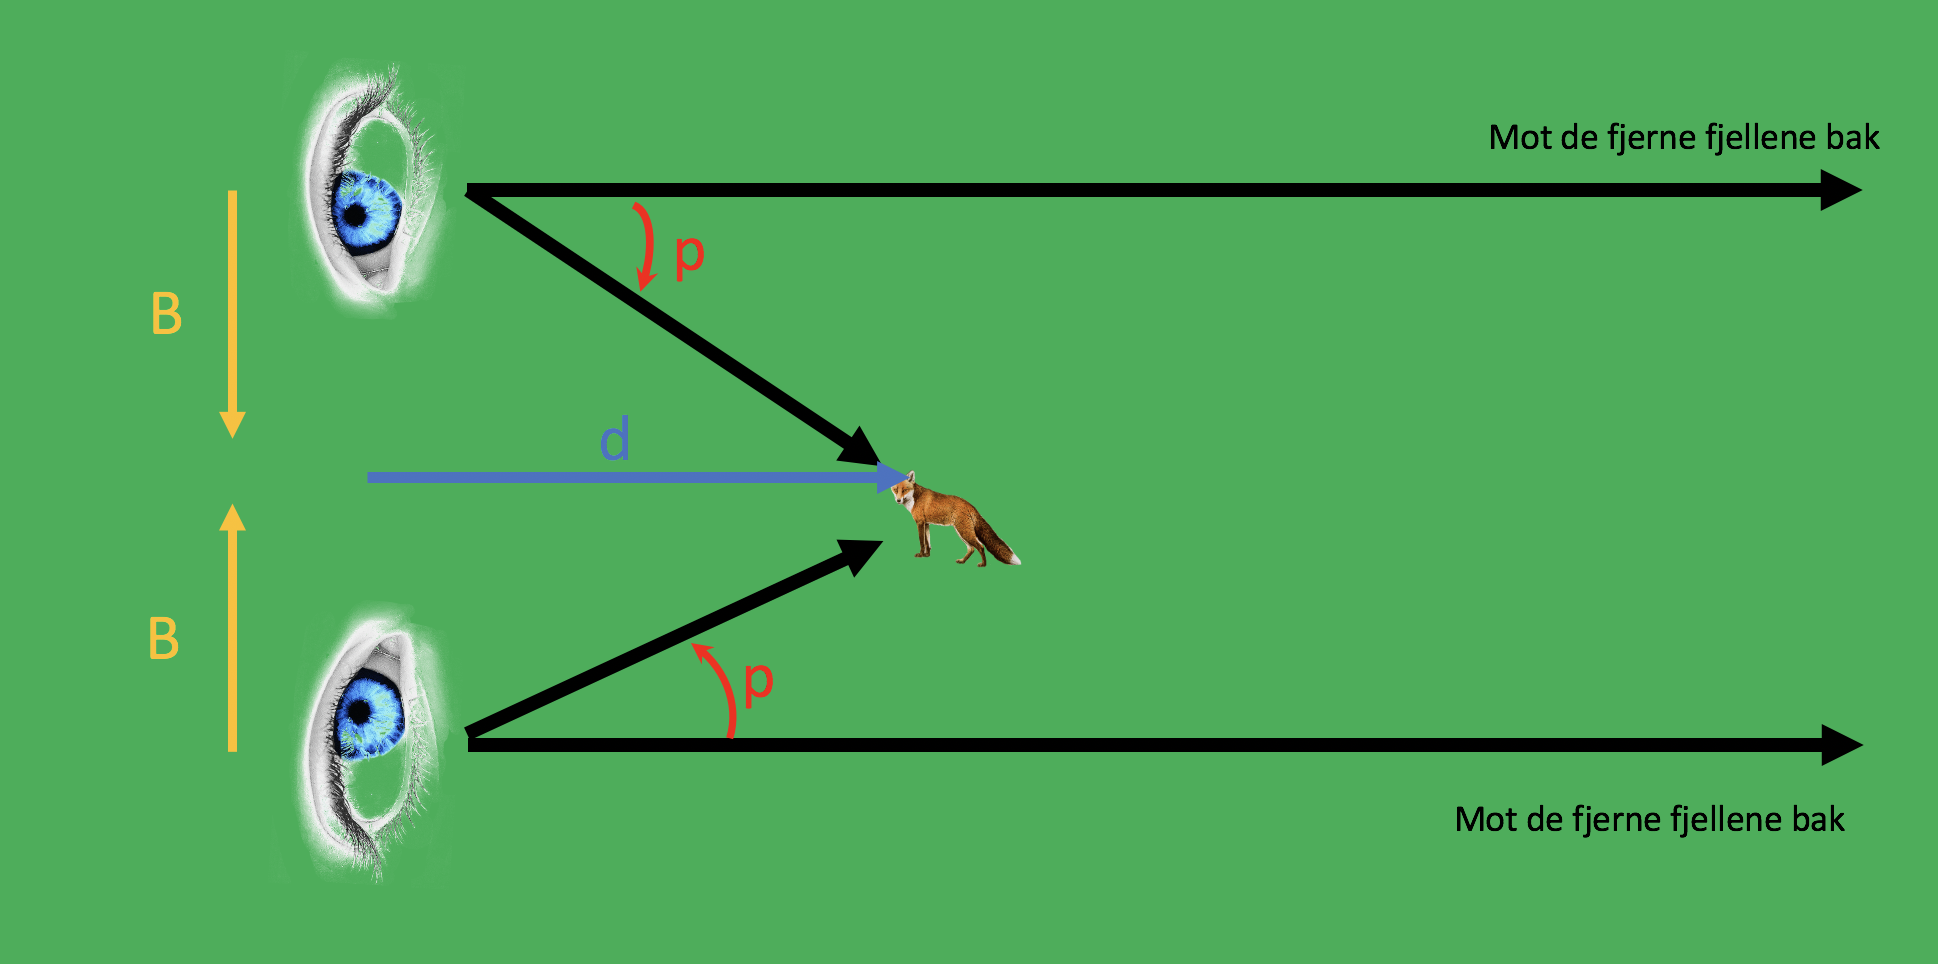
\includegraphics[scale=0.3]{media/fox_eyes_distance.png}}
Helt riktig! Her er det fort gjort å trå feil: Husk at {\bf $B$ er avstanden fra nese til øye}, $2B$ er avstand fra øye til øye. Og {\bf parallaksevinkelen $p$ er definert som vinkelen fra to øyer (altså midten) til et øye} mens $2p$ er vinkelen fra øye til øye! Ser du det på figuren? Dette er en veldig typisk feil på eksamen, pass på at du alltid tegner figur og er klar over hva definisjonene av baseline $B$ og parallaksevinkel $p$ er.
\hyperlink{paral14}{\pagebutton{Neste side}}
\end{frame}
}


\begin{frame}
\label{paral14}
\lastpagebutton{riktig_paral13b}
Vi ser at parallaksemålinger kan brukes til å bestemme avstander! Nettopp det vi trengte! {\bf Men hvordan kan vi nå bruke dette i astrofysisk sammenheng?} Tenk deg at du har en stjerne i Melkeveien, og så ser du den i forhold til en fjern, fjern galakse! \textcolor{red}{Hvis du nå tar bilde med to teleksoper som har en stor avstand fra hverandre, så vil du vel få samme effekt som med reven?} {\bf MEN, hvis parallaksevinkelen $p$ er liten, mindre enn oppløsningsevnen til teleskopet, ja da vil du vel ikke kunne se stjernas ``bevegelse'' i forhold til den fjerne galaksen?} Hvis du husker fra diskusjonen om ekstrasolare planeter, så vil en parallaksevinkel som er mindre en oppløsningsvinkelen til teleskopet bety at stjerna da vil se ut til å være på samme plass på bildet og vi kan ikke måle parallaksevinkel!. \textcolor{red}{\bf For at vi skal kunne bruke parallakse for å måle avstander til astronomiske objekter, må vi derfor sørge for en stor parallaksevinkel $p$}. Men hvordan kan vi få til det?? La oss se på formelen igjen:
\[
B=dp\ \ \ \textrm{(hvor\ p\ må\ være\ i\ radianer)}
\]
{\bf Hvordan kan du sørge for at parallaksevinkelen er stor når du skal måle avstanden til f.eks. en stjerne?}
\hyperlink{feil_paral15}{\pagebutton{\small Jeg har et svar!}}
\end{frame}

{
\setbeamercolor{background canvas}{bg=black}
\begin{frame}
\label{feil_paral15}
\lastpagebutton{paral14}
\centerline{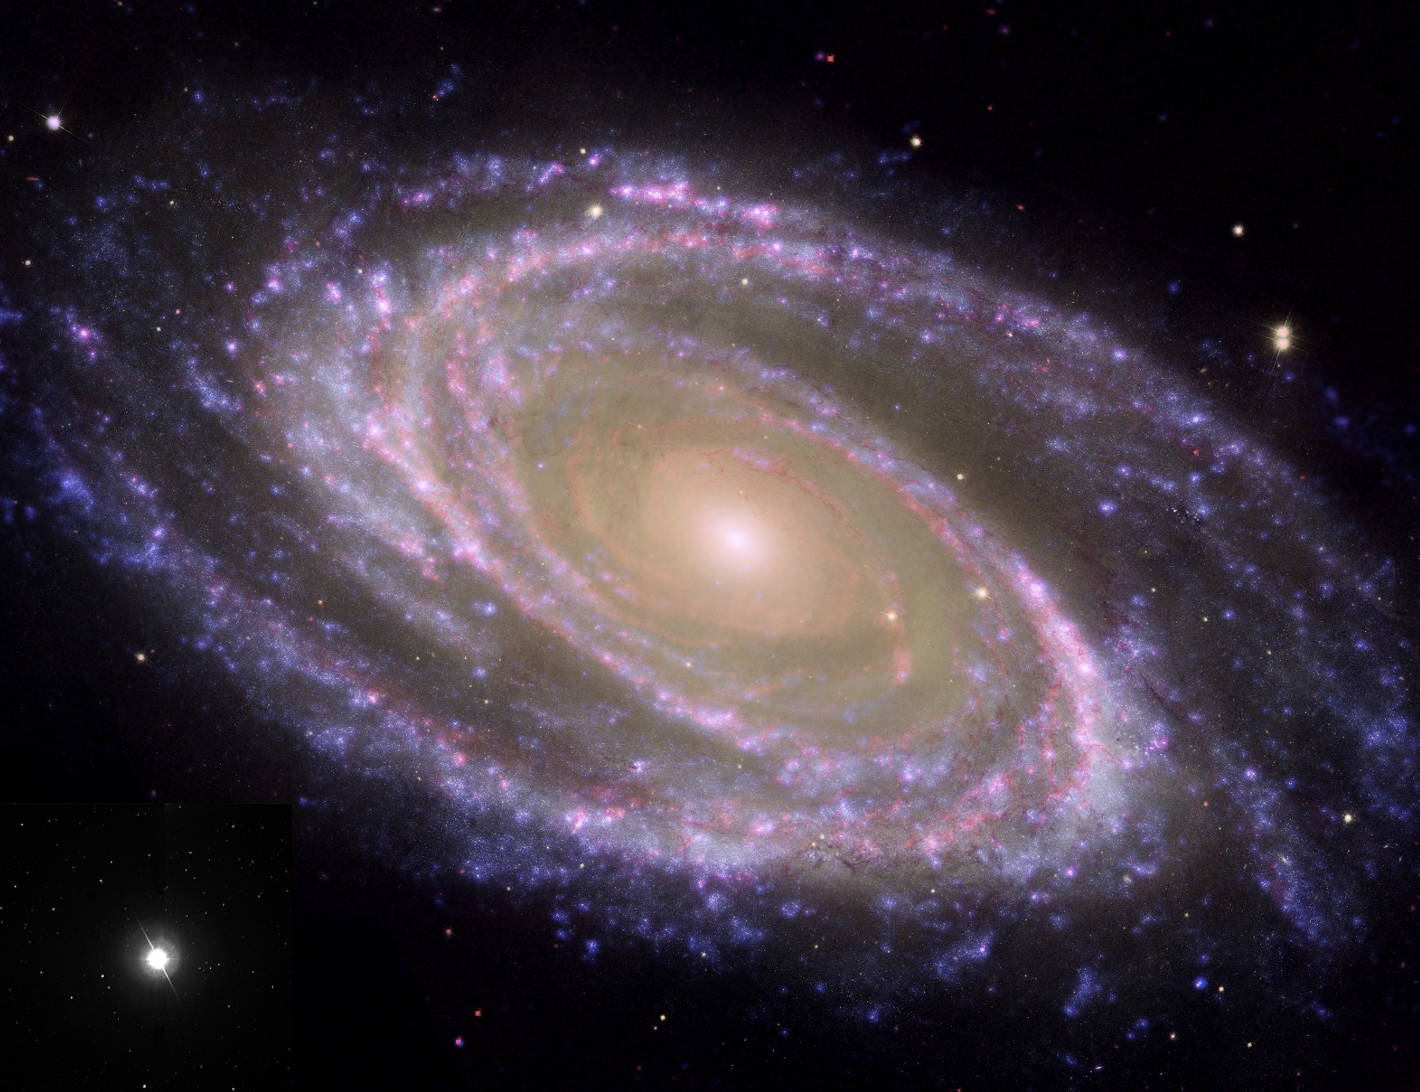
\includegraphics[scale=0.2]{media/galaxy_left.png}}
\textcolor{yellow}{La oss først se på et eksempel. Ovenfor ser du et bilde tatt fra et teleskop med en fjern galakse i bakgrunnen og en ``nær'' stjerne nederst til venstre. Hvis nå et annet teleskop som står et annet sted tar et bilde i samme retning, hvordan vil det set ut?}\hyperlink{feil_paral15b}{\pagebutton{\small Jeg vet det!}}\\
{\footnotesize\textcolor{yellow}{Bilde: NASA/JPL-Caltech/ESA/Harvard-Smithsonian CfA }}

\end{frame}
}


{
\setbeamercolor{background canvas}{bg=black}
\begin{frame}
\label{feil_paral15b}
\lastpagebutton{feil_paral15}
%\centerline{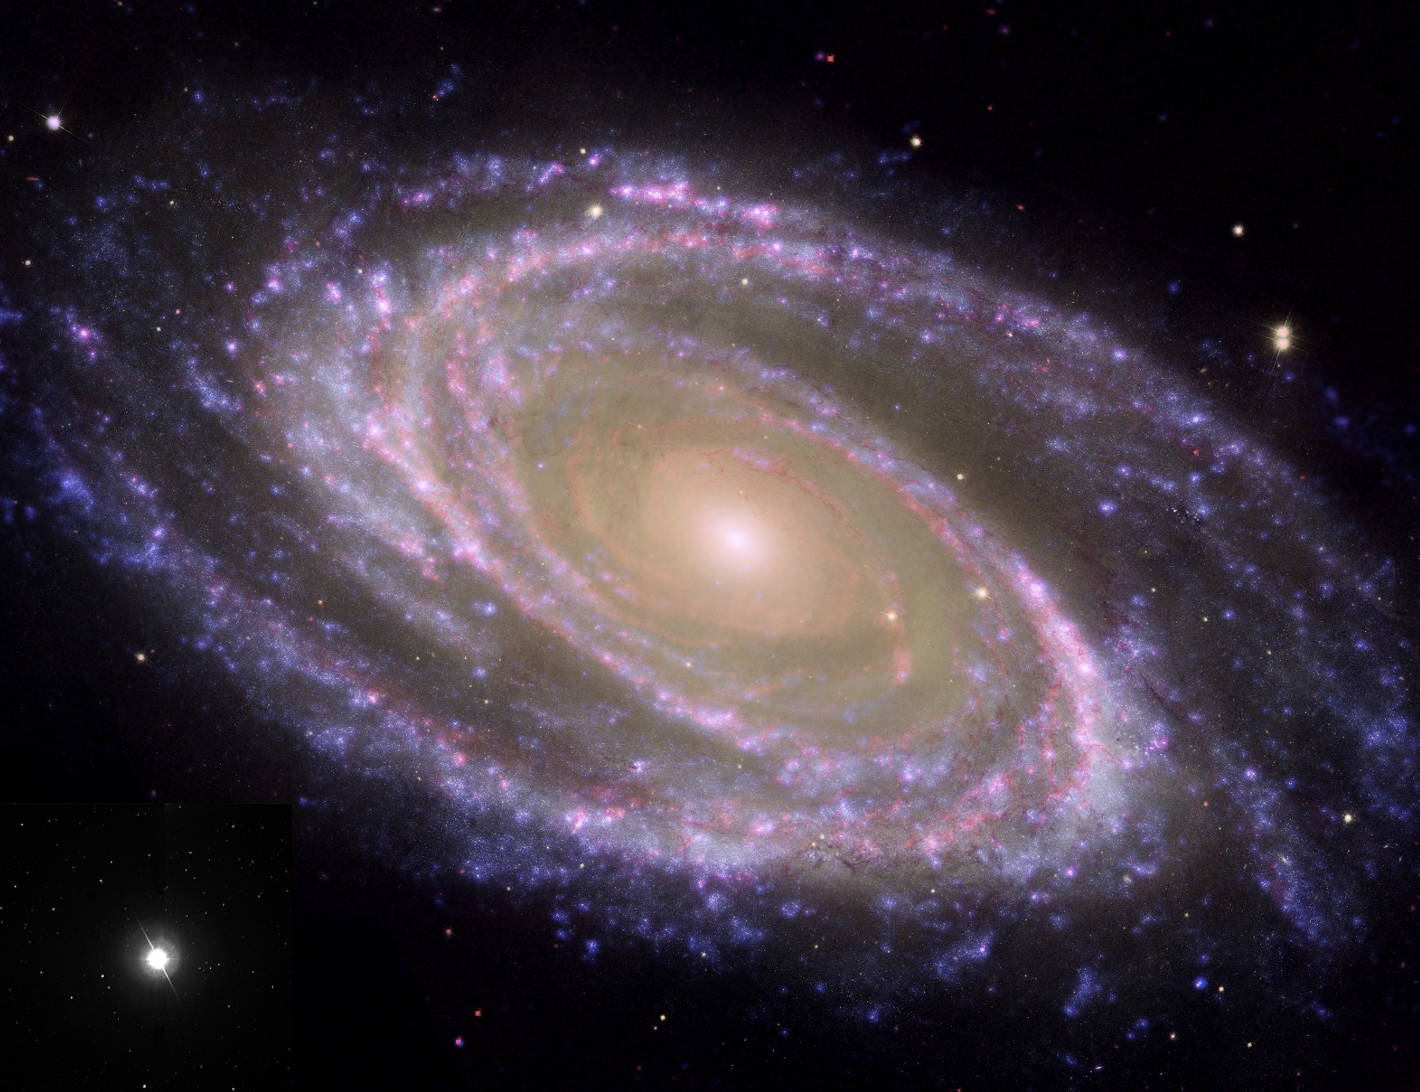
\includegraphics[scale=0.2]{media/galaxy_left.png}\ 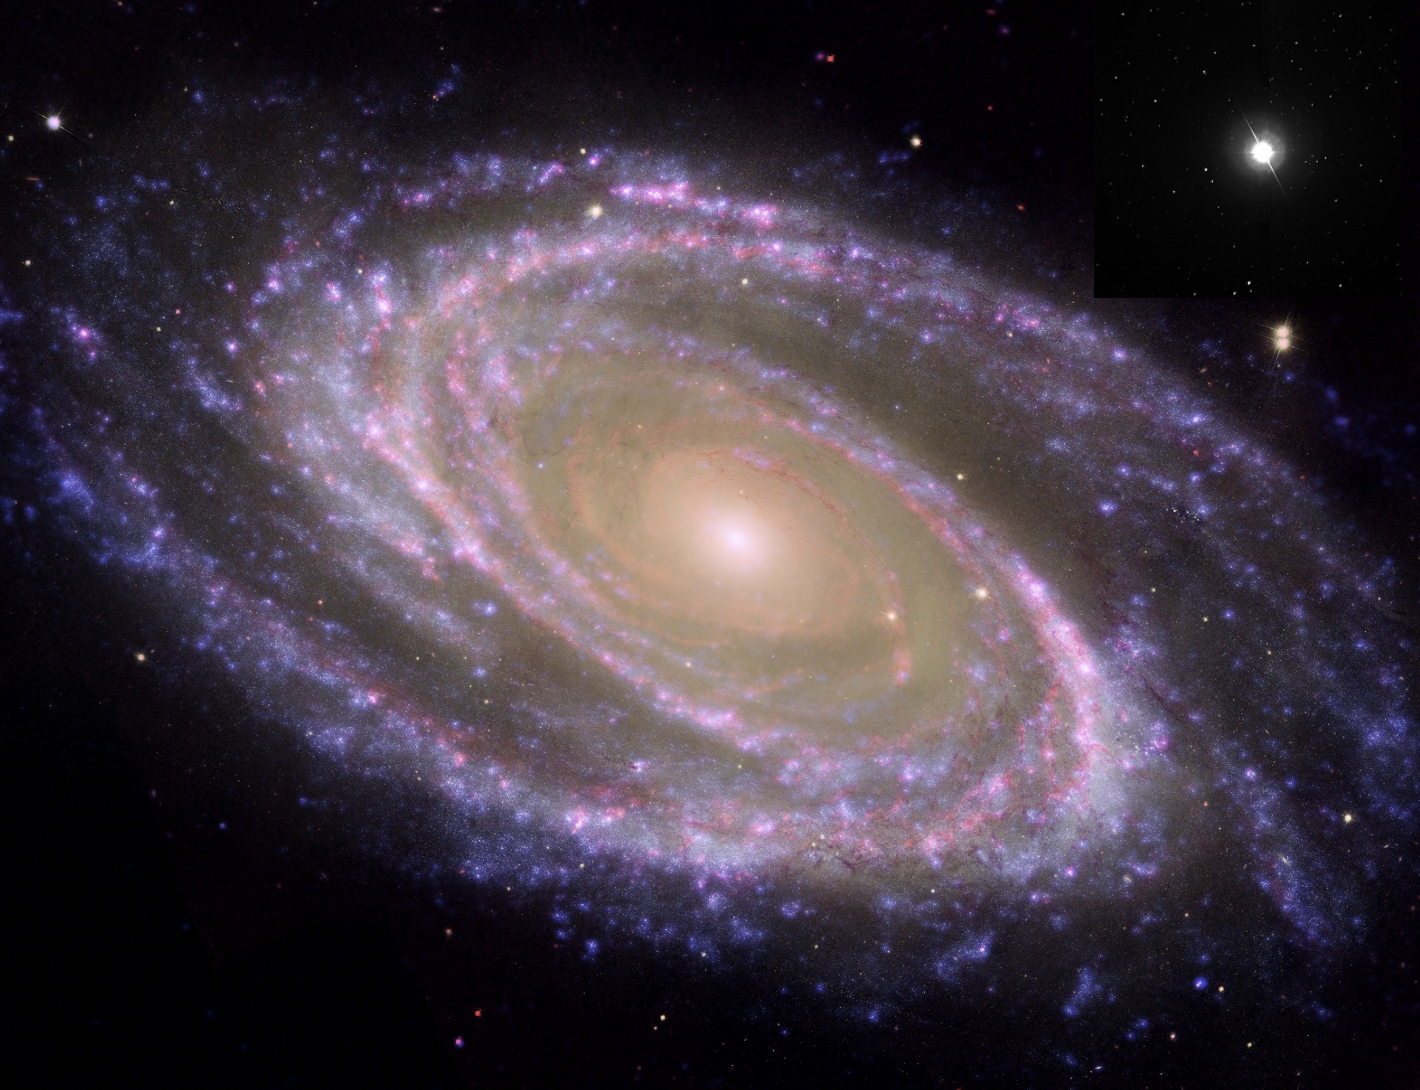
\includegraphics[scale=0.2]{media/galaxy_right.png}}
\centerline{\includegraphics[scale=0.2]{media/galaxy_comb.png}}
\textcolor{yellow}{Nettopp ja! Her ser du bildene fra begge teleskopene! {\bf Ser du hvordan stjerna står på et annet sted i forhold til den fjerne galaksen, på samme måte som reven?}. Men hvis parallaksevinkelen $p$ hadde vært mye mindre så ville ikke stjerna flyttet på seg like mye, og kanskje ville den tilsynelatende (innenfor oppløsningsevnen til teleskopet) stått på samme sted. Derfor er det viktig å få denne vinkel (forflytningen) stor nok. Så da spør jeg en gang til, hva kan man gjøre for å få størst mulig $p$ for et objekt slik at parallakseeffekten blir synlig?
\[
B=dp\ \ \ \textrm{(hvor\ p\ må\ være\ i\ radianer)}
\]}
\hyperlink{paral16}{\pagebutton{\small Jeg har et svar!}}
\end{frame}
}


\begin{frame}
\label{paral16}
\lastpagebutton{feil_paral15}
{\small
Hvis vi skriver om formelen
\[
p=\frac{B}{d}
\]
ser vi at {\bf stor $B$} eller {\bf liten $d$} vil gjør parallaksevinkelen $p$ stor. Det med liten avstand $d$ er ikke noe vi kan bestemme, det er jo bare så langt unna objektet er. Hvis objektet er langt unna, vil vi ikke få en parallaksevinkel stor nok til at parallakseeffekten kan observeres. \textcolor{red}{ Dermed ser vi at parallaksemålinger har en sterk begrensning: den kan kun brukes på objekter som er nærme (vi skal snart se hvor nærme). Derfor er denne metoden det første steget på avstandsstigen.} Vi må altså akseptere avstanden som det den er. Det eneste vi dermed kan endre på er baseline $B$. Husk at avstanden mellom øynene/teleskopene er $2B$. Vi må altså ha teleskopene så langt fra hverandre som bare mulig. \textcolor{blue}{La oss gjøre overslagsregning her: Jordas radius er ca.6000km. Hvis vi antar at vi har et teleskop på hver kant av jorda slik at avstanden mellom disse er 12000km, og vi hadde en begrensing på oppløsningsevnen til atmosfæren på ca. 0.4'', {\bf hva er da avstanden til den fjerneste stjernen som vi kan måle en parallakseeffekt på?} Altså hvor langt ut i universet kan vi se effekten av parallakse, og dermed måle avstanden med denne metoden, hvis vi maks klarer å se en ``forflytning'' av stjerna  mellom de to bildene som er større enn 0.4''? Gi svaret i lysår}
}
\hyperlink{paral17}{\pagebutton{\small Jeg har et svar!}}
\end{frame}


\begin{frame}
\label{paral17}
\lastpagebutton{paral16}
Fikk du omkring 0.0003 lysår??
\[
d=\frac{B}{p}=\frac{12000\,\mathrm{km}}{\frac{0.4}{3600}\frac{\pi}{180}}=\frac{6187944187412\mathrm{m}}{3\times10^8\,\mathrm{m/s}\times365\times24\times3600\,\mathrm{s}}\mathrm{ly}=0.00065\,\mathrm{ly}
\]
Den nærmeste stjerna til sola er omkring 4 lysår unna, men med parallakse kan vi altså kun måle avstander som er mye mindre enn dette! {\bf En fullstendig ubruklig metode altså?} \textcolor{red}{ELLER... når jeg tenker meg om så finnes det en måte å få teleskopene {\bf enda} lenger fra hverandre på! Faktisk så mye lenger fra hverandre at vi kan måle parallakse til de nærmeste stjernene!} Og det uten å sende noe som helst ut i verdensrommet! {\bf Nå fikk du litt å gruble på her...} Hvis du ikke ser det, ta deg en 10 min. spasertur, eller gå og lag deg en te, og {\bf tenk}. Hvilket triks kan vi gjøre her?
\hyperlink{paral18}{\pagebutton{\small Jeg har tenkt meg godt om...}}
\end{frame}


\begin{frame}
\label{paral18}
\lastpagebutton{paral17}
\centerline{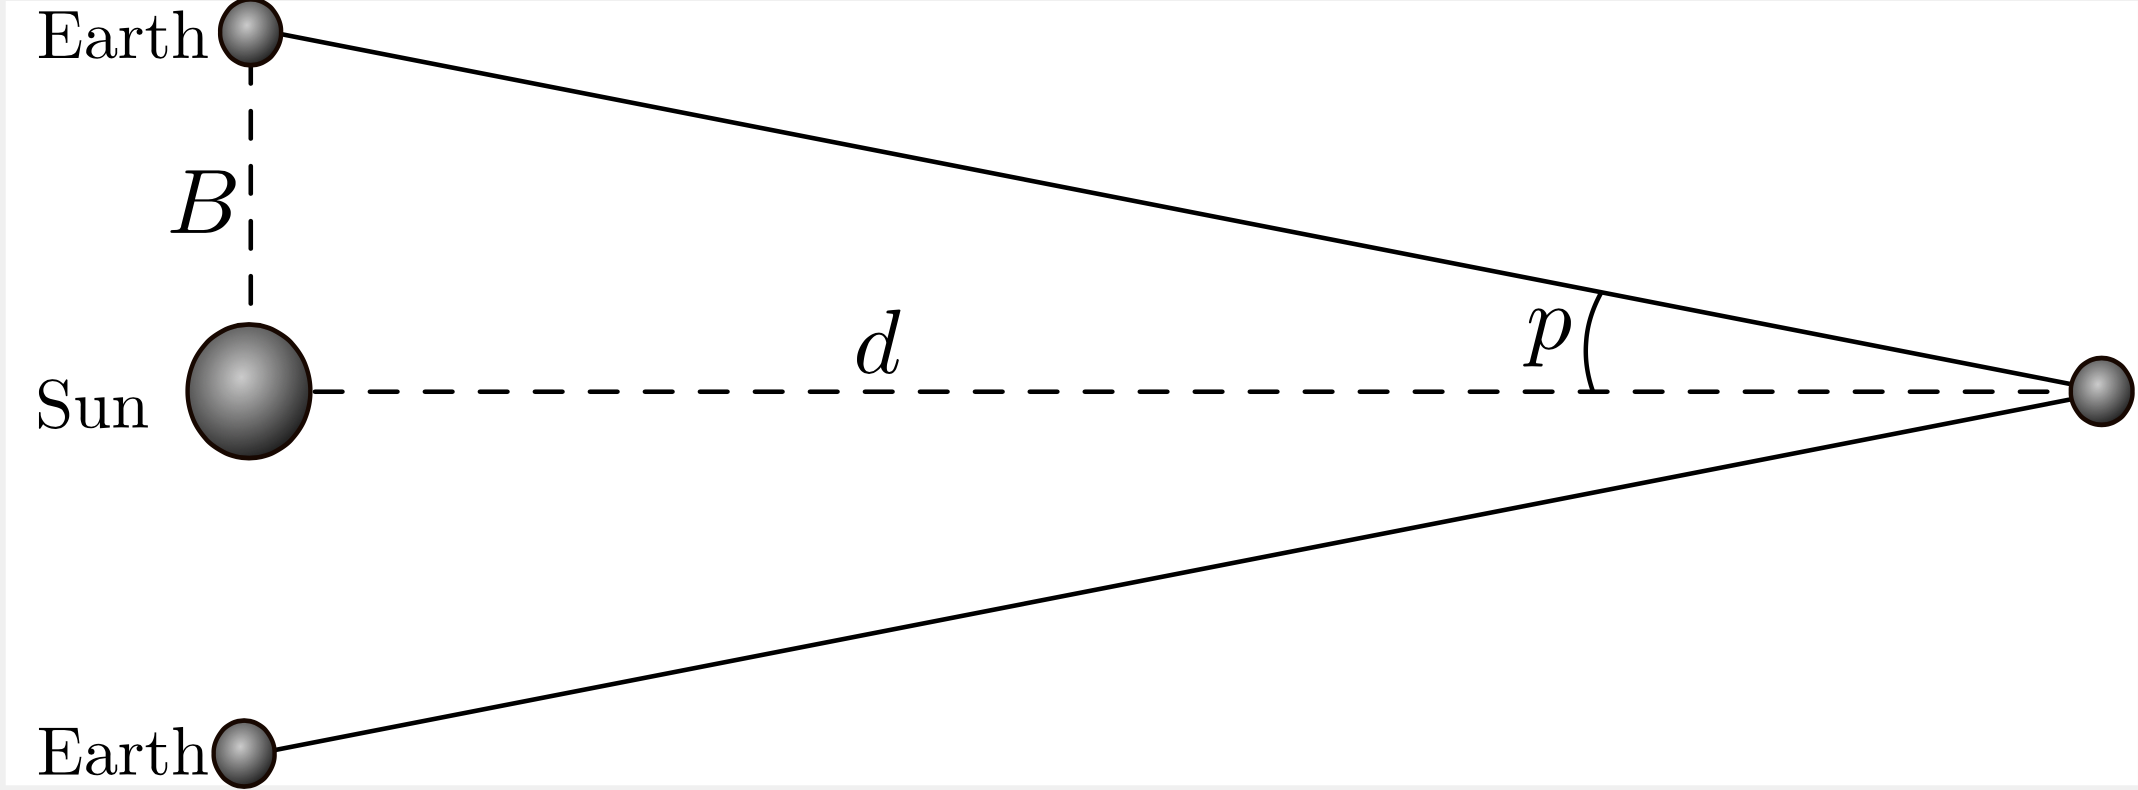
\includegraphics[scale=0.8]{media/fig_11-2.png}}

{\Large {\bf GENIALT!} Hvis vi tar bildet med 6 måneders mellomrom, så få vi en baseline på 1AU!}
{\small Hvis vi gjør regninga vår på nytt med en baseline på 1AU så ser vi at vi kan måle avstander til stjerner i en avstand i omkring 10 lysår. I virkeligheten er ikke vinkelen 0.4'' absolutt her, man kan skille vinkler mindre enn dette med god bildebehandling og dataanalyse slik at man kan bruke dette med avstander på flere titalls lysår. Med romobservatoriet \href{https://en.wikipedia.org/wiki/Gaia_(spacecraft)}{Gaia} (skutt opp i 2013) som er utenfor atmosfæren og i tillegg bruker teknikker som ved å observere objektene mange, mange ganger gjør at man nå kan måle parallakseeffekter så små at vi kan bruke parallakse til å måle avstander til objekter i hele Melkeveien.}
\hyperlink{paral19}{\pagebutton{\small Neste side}}
\end{frame}



\begin{frame}
\label{paral19}
\lastpagebutton{paral18}
\centerline{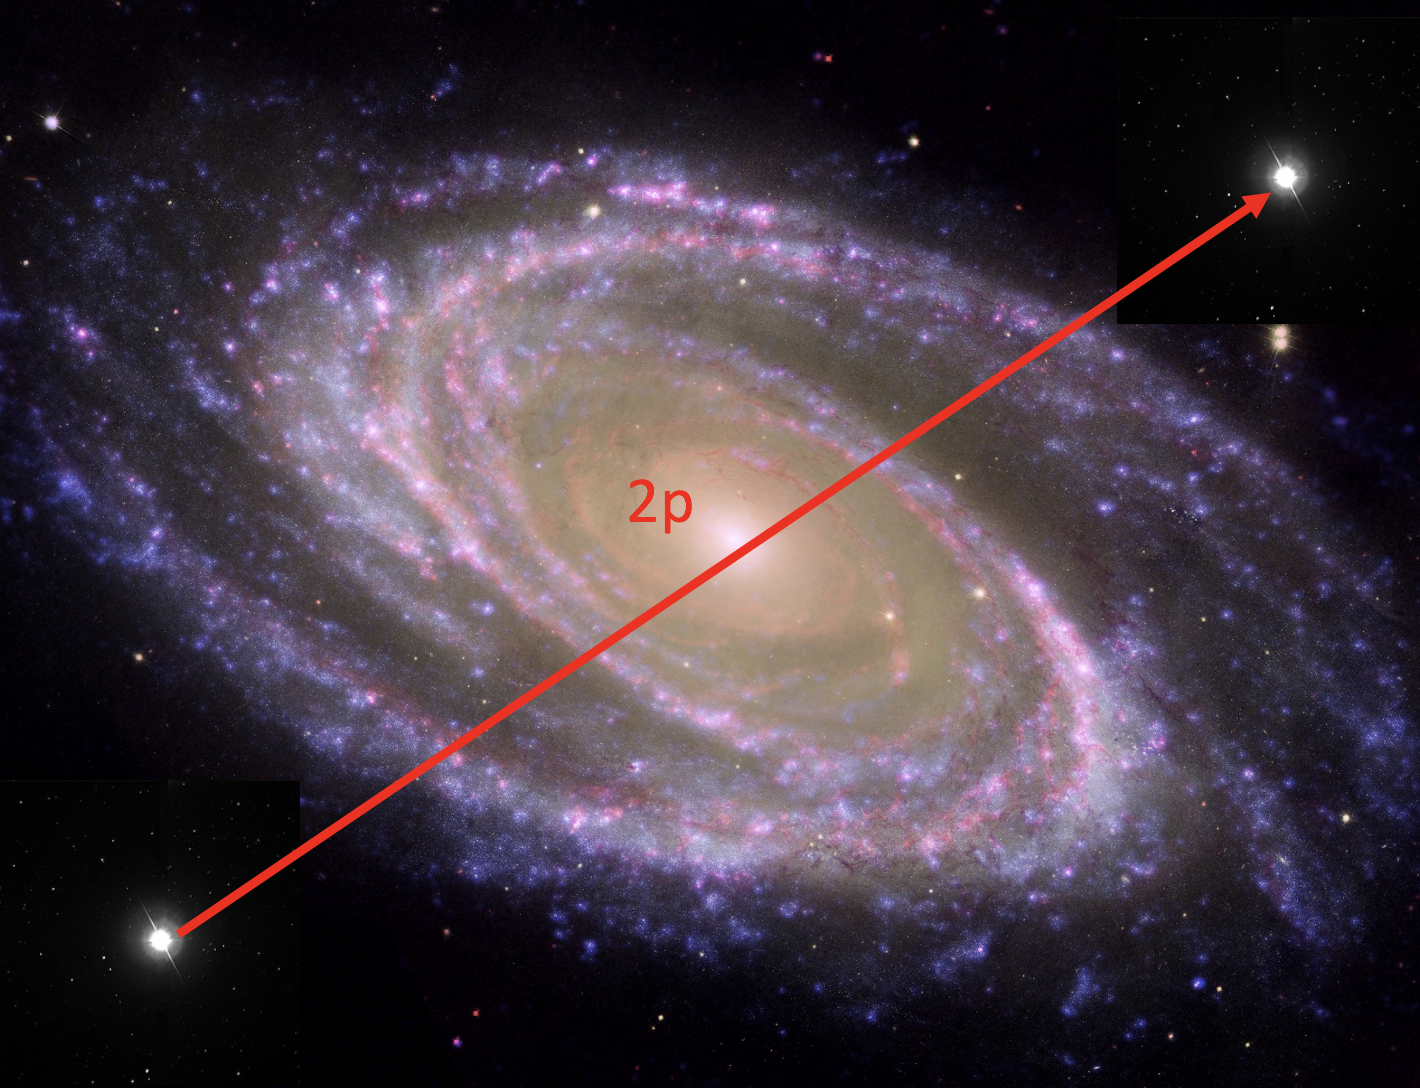
\includegraphics[scale=0.3]{media/galaxy_both.png}}
Her ser vi stjerna med galaksen i bakgrunnen igjen, der bildene nå er lagt over hverandre slik at vi ser stjerna i begge posisjoner. Dette bildet er tatt med det samme teleskopet med 6 måneders mellomrom. Vinkelavstanden mellom de to stjernene på det sammensatte bildet her er 0.1''. Hvor langt unna er stjerna?
\hyperlink{paral19a}{\choicebutton{ca. 32\,ly}}\ \ \ \hyperlink{riktig_paral19b}{\choicebutton{ca. 65\,ly}}\ \ \ \hyperlink{paral19a}{\choicebutton{ca. 130\,ly}}\ \ \ \hyperlink{paral19a}{\choicebutton{ca. 260\,ly}}\ \ \ \hyperlink{paral19a}{\choicebutton{ca. 520\,ly}}\ \ \ 
\end{frame}

\begin{frame}
\label{paral19a}
\lastpagebutton{paral19}
\centerline{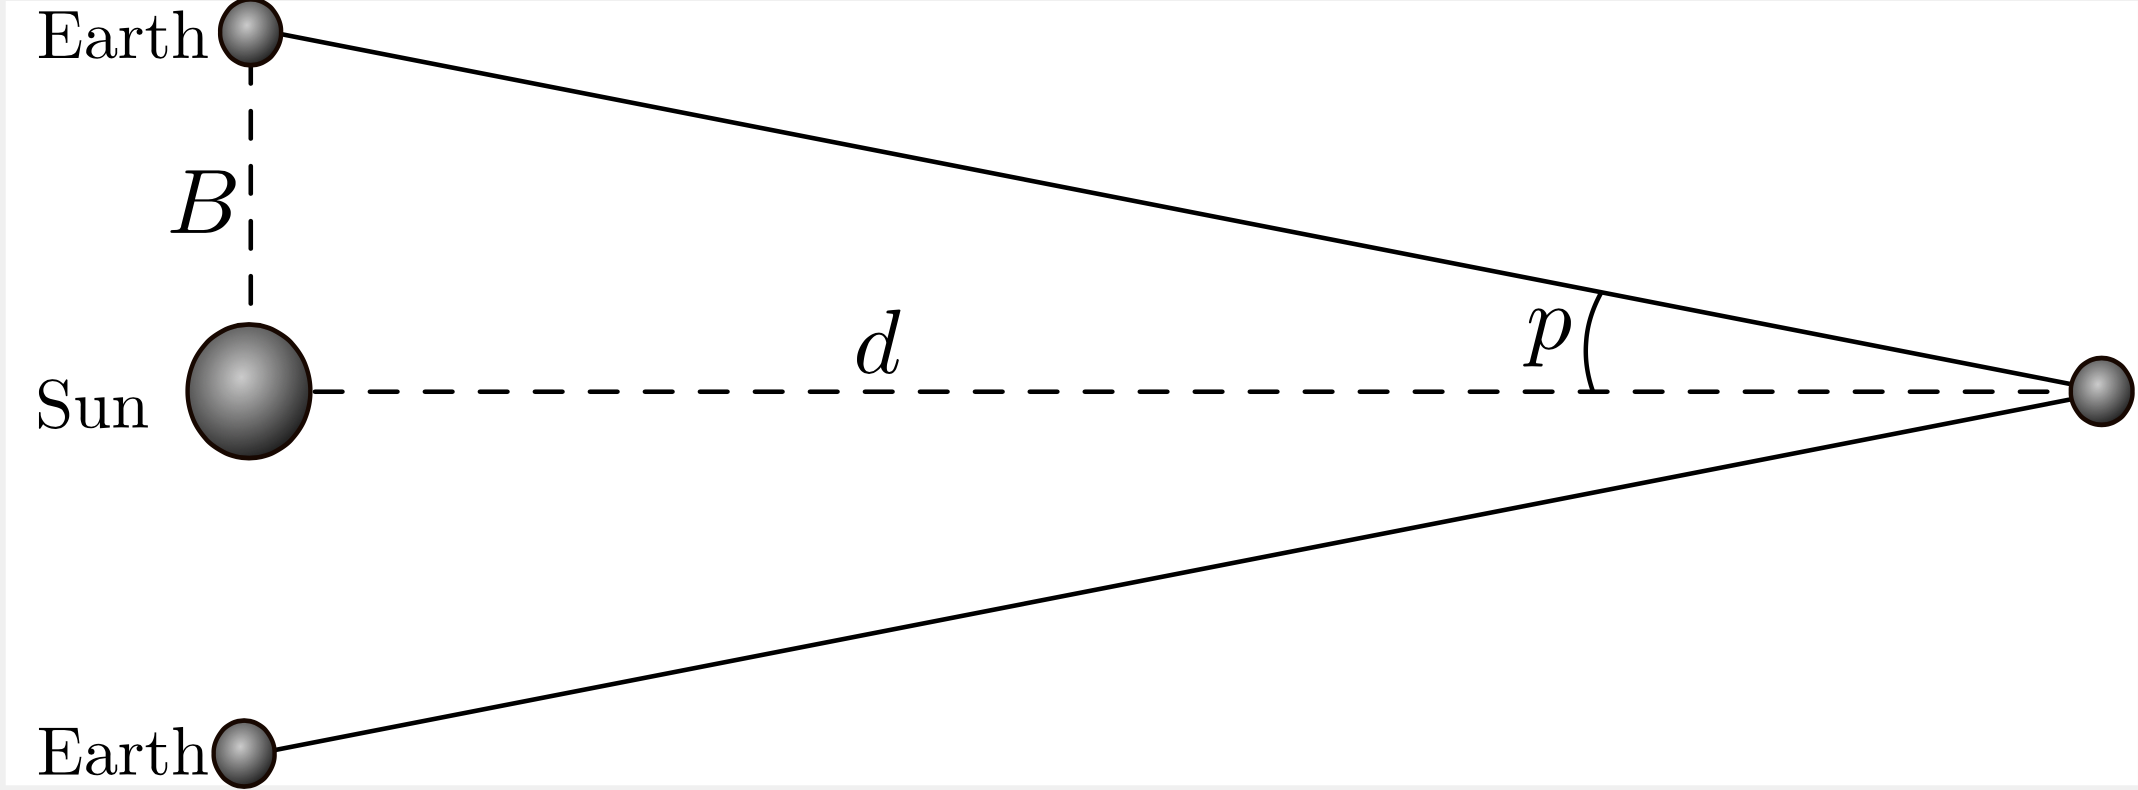
\includegraphics[scale=0.8]{media/fig_11-2.png}}
\Large Har du glemt en faktor 2 et eller annet sted??? Eller hvordan var det med omregning fra buesekunder til grader til radianer? Eller omregning til lysår?
\end{frame}

{
\setbeamercolor{background canvas}{bg=yellow}
\begin{frame}
\label{riktig_paral19b}
\clastpagebutton{paral19}
Det er helt riktig! Da fikk du faktorene 2 rett! Og du fikk regnet riktig om til radianer. Gratulerer du har tatt det første steget ut i verdensrommet.
\hyperlink{paral19c}{\pagebutton{Neste side}}
\end{frame}
}


\begin{frame}
\label{paral19c}
\lastpagebutton{riktig_paral19b}
Da er du klar for å se hvor definisjonen av {\bf parsec} kommer fra. Smak litt på ordet...{\bf par} og {\bf sec}. Hva med {\bf par}allakse per bue{\bf sek}und. Nettopp! Hvis en stjerne har \textcolor{red}{en parallakse på et buesekund, så er avstanden til stjernen en parsec!}. Og da går vi utifra en baseline B=1AU. La oss se:
\[
d=\frac{B}{p}=\frac{1AU}{p}=\frac{1AU}{p''\frac{1}{3600}\frac{\pi}{180}}=\frac{206265}{p''}AU
\]
der $p''$ er parallaksevinkelen målt i buesekunder. Hva blir da avstanden til en stjerne med parallakse på 0.1''?
\hyperlink{paral19_d}{\pagebutton{Jeg tror jeg vet det!}}\\
\textcolor{white}{
Fikk du 10pc? Det skulle du!
Neste side}
\end{frame}

\begin{frame}
\label{paral19_d}
\lastpagebutton{riktig_paral19b}
Da er du klar for å se hvor definisjonen av {\bf parsec} kommer fra. Smak litt på ordet...{\bf par} og {\bf sec}. Hva med {\bf par}allakse per bue{\bf sek}und. Nettopp! Hvis en stjerne har \textcolor{red}{en parallakse på et buesekund, så er avstanden til stjernen en parsec!}. Og da går vi utifra en baseline B=1AU. La oss se:
\[
d=\frac{B}{p}=\frac{1AU}{p}=\frac{1AU}{p''\frac{1}{3600}\frac{\pi}{180}}=\frac{206265}{p''}AU
\]
der $p''$ er parallaksevinkelen målt i buesekunder. Hva blir da avstanden til en stjerne med parallakse på 0.1''?
{\pagebutton{Jeg tror jeg vet det!}}\\
Fikk du 10pc? Det skulle du!
\hyperlink{feil_nytema2}{\pagebutton{Neste side}}
\end{frame}



\renewcommand{\headline}{\small hovedserietilpasning}
{
\setbeamercolor{background canvas}{bg=black}
\begin{frame}
\label{feil_nytema2}
\begin{columns}
\column{0.5\textwidth}
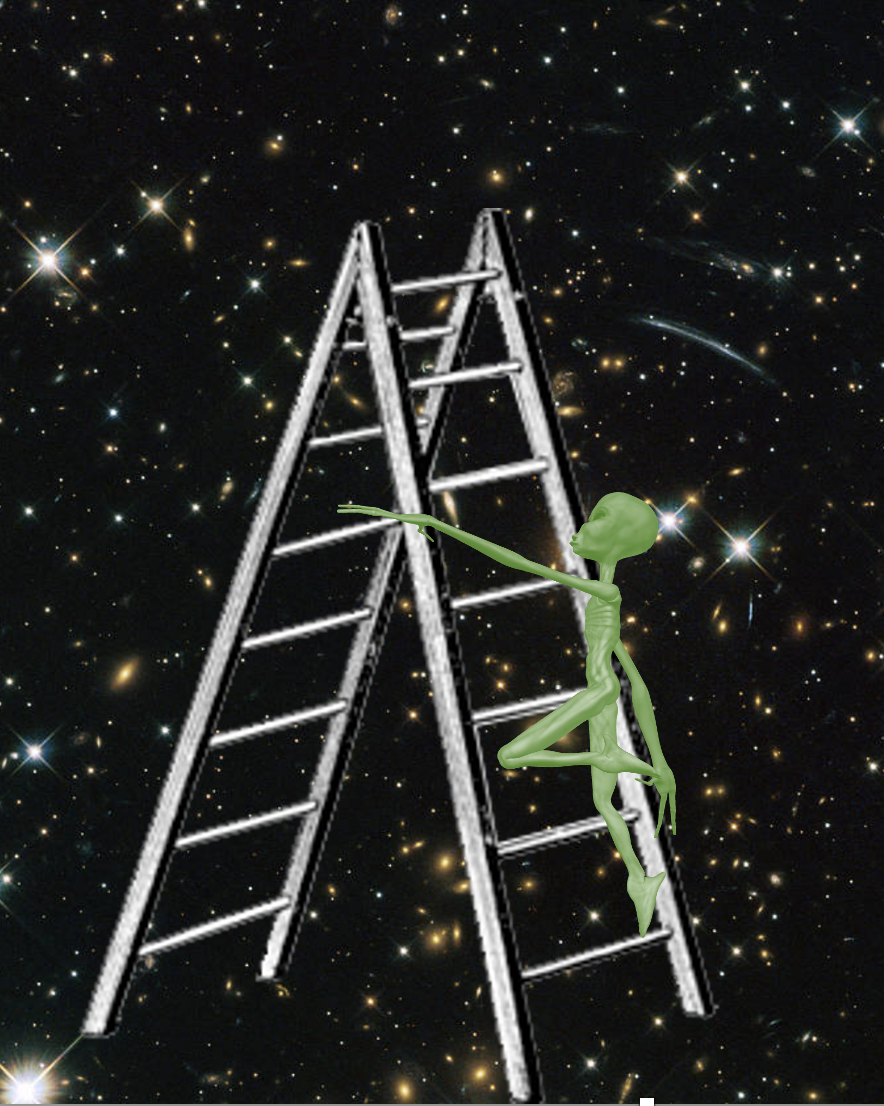
\includegraphics[scale=0.4]{media/ladder2.png}
\hyperlink{riktig_paral19b}{\pagebutton{\small Forrige side}}
\column{0.5\textwidth}
\textcolor{red}{\small Vi tar det andre steget på avstandsstigen:}\vspace*{1cm}
\nytemaside{cepheider}
\textcolor{red}{\Large Nå må du ta en strekk på bena før du går videre her!!!}
\hyperlink{msfit1}{\pagebutton{La oss klatre videre!}}
\end{columns}
\end{frame}
}


\begin{frame}
\label{msfit1}
\dlastpagebutton{riktig_paral19b}\label{hrfit}
{\Huge Hovedserietilpasning????}
La oss dele opp ordet:{\bf Hovedserie}-tilpasning.
Dette med tilpasning kan man kanskje få noe ut av men for å forstå hva hovedserien er, så trenger vi å bruke Hertzspring-Russel-diagrammet!
\hyperlink{msfit2}{\pagebutton{Hvafforno'???}}
\end{frame}

\begin{frame}
\label{msfit2}
\lastpagebutton{msfit1}
{\Huge Hertzsprung-Russel-diagrammet????}
Jepp, tida har kommet til å introdusere dere til et av de viktigste redskaper for å studere stjerners liv og virke. Men for å forstå hva et Hertzsprung-Russel-diagram, eller bare {\bf HR-diagram}, er så trenger du å vite hva en stjernehop er, eller rettere sagt hva en åpen hop og en kulehop er.
\hyperlink{msfit3}{\pagebutton{Hvafforno'???}}
\end{frame}

\begin{frame}
\label{msfit3}
\lastpagebutton{msfit2}
{\Huge Stjernehop????}
Hva i alle dager er det...
\hyperlink{msfit4}{\pagebutton{...for noe???}}
\end{frame}


\begin{frame}
\label{msfit4}
\lastpagebutton{msfit3}
En {\bf stjernehop} er en samling av noen hundre eller noen tusen stjerner som alle ble født omtrent samtidig av den samme gass-skya. En stor kuleformet gassky med masse på flere tusen solmasser kollapset under sin egen gravitasjon og ble fragmentert i mindre kuleformede skyer som dannet stjerner. Stjernehoper kan deles inn i to grupper:
\begin{itemize}
\item {\bf Kulehoper (``globular clusters'' på engelsk):} Disse går i bane rundt en galakse, ofte langt fra galaksens sentrum og ofte har de baner utenfor galakseplanet. De har beholdt sin opprinnlige kuleform og er derfor en kuleformet ansamling av stjerner, derav navnet.
\item {\bf Åpne hoper} ble dannet i galakseskiven og har med tiden blitt ``revet i stykker'' av gravitasjonskrefter fra nærliggende objekter eller tidevannskrefter fra galaksens sentrum. Disse har dermed ikke lenger kuleform, men har blitt ``åpnet opp'' og fått en irregular form.
\end{itemize}
\hyperlink{feil_msfit5}{\pagebutton{Neste side}}
\end{frame}


{
\setbeamercolor{background canvas}{bg=black}
\begin{frame}
\label{feil_msfit5}
\lastpagebutton{msfit4}
\centerline{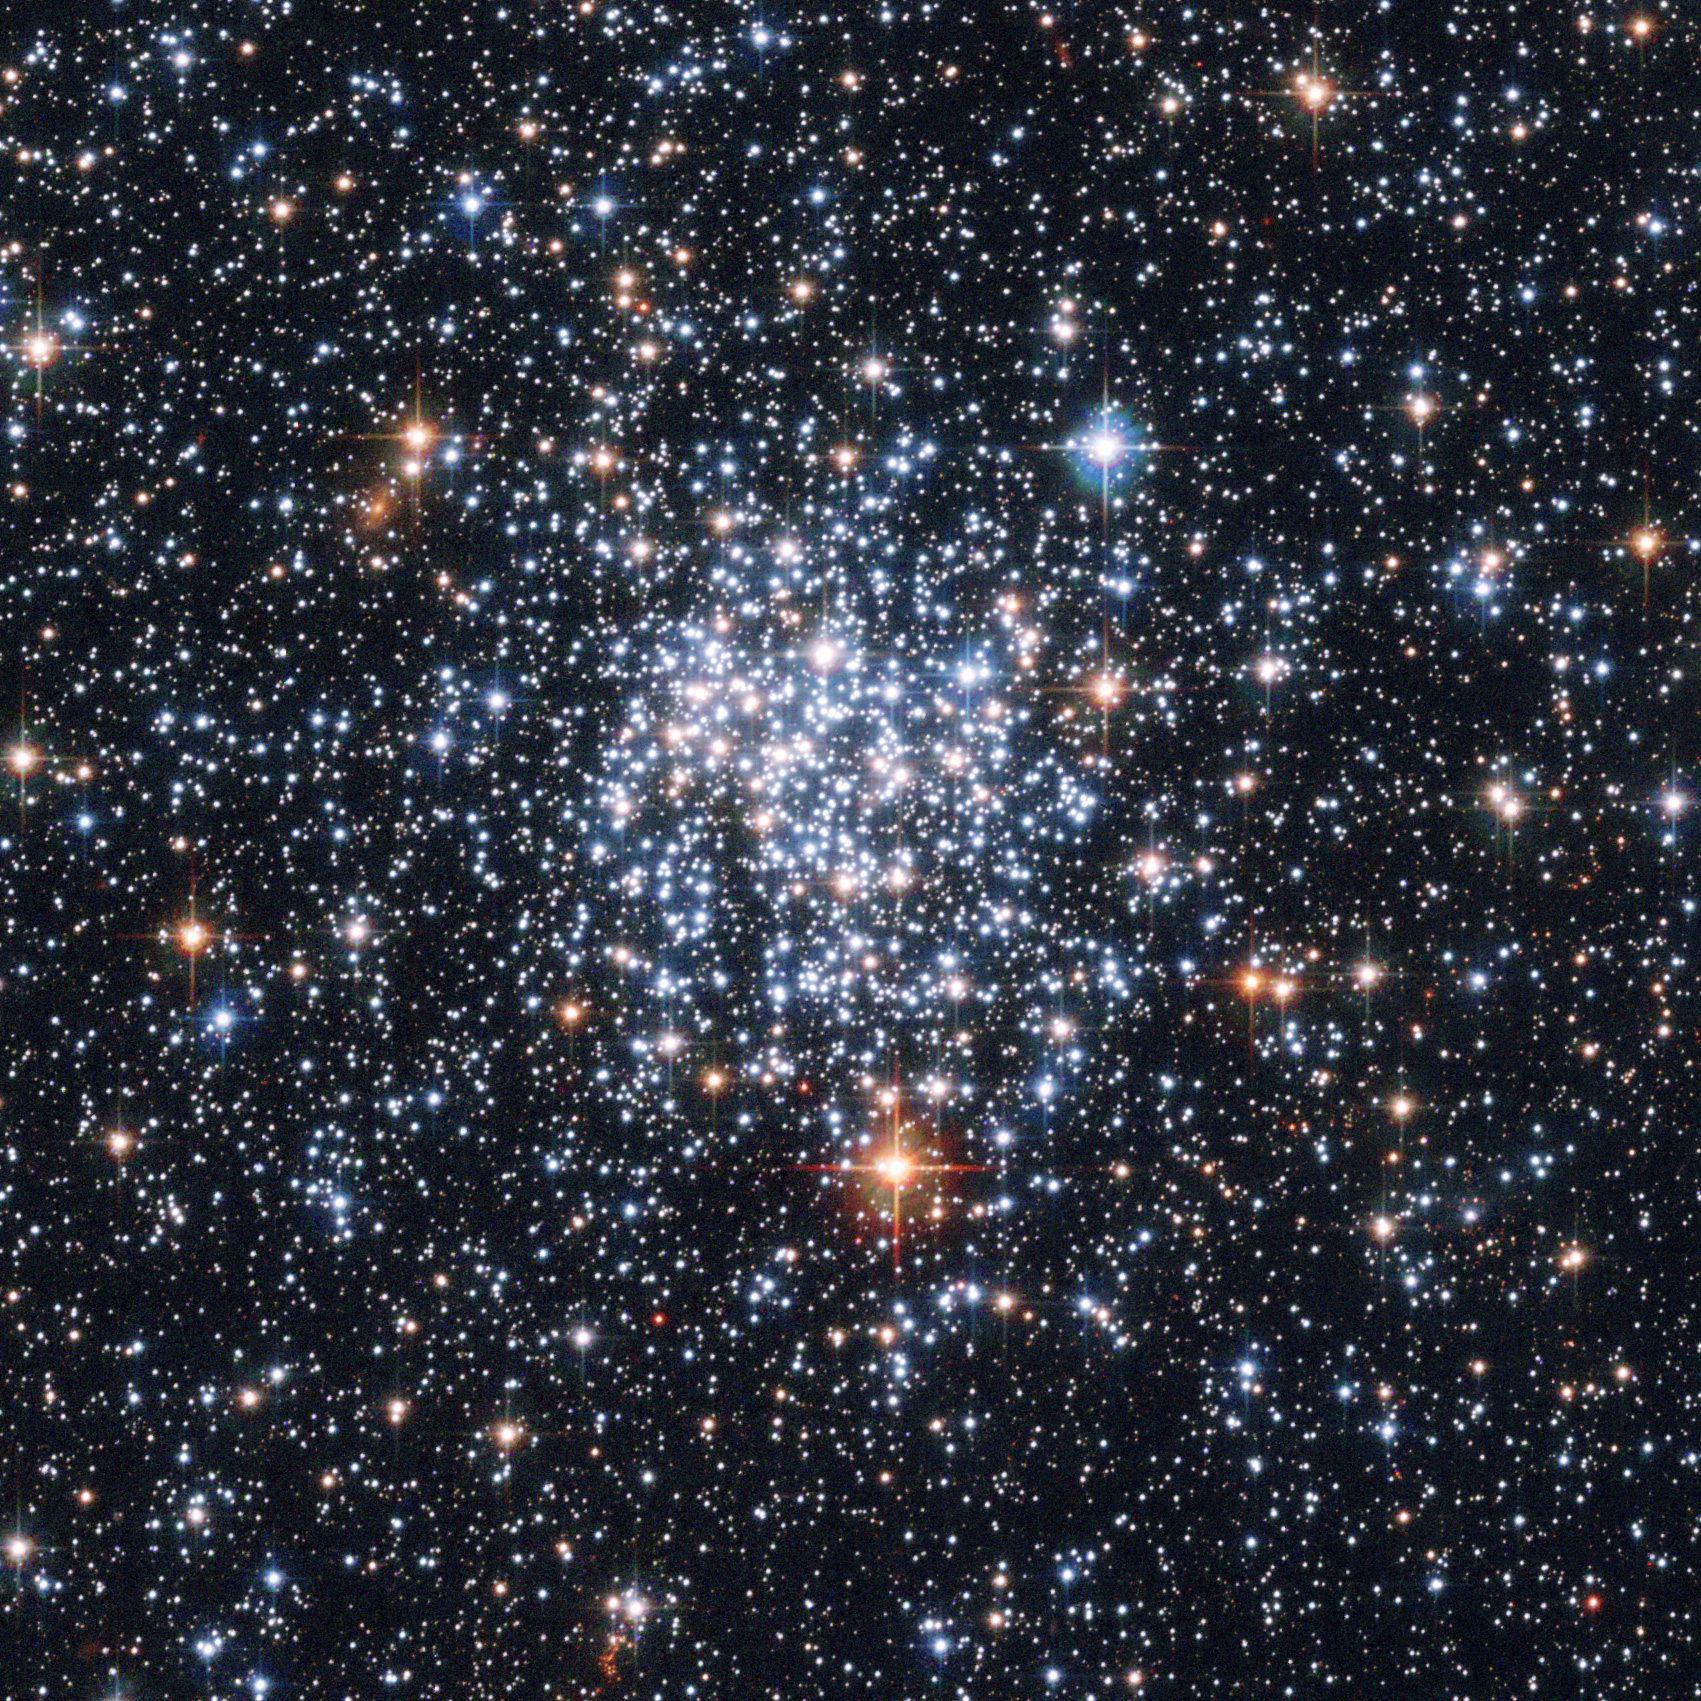
\includegraphics[scale=0.09]{media/open_cluster_NGC265.jpg}}
\textcolor{yellow}{Her ser vi en åpen hop, kalt NGC265. Denne åpne hopen ligger faktisk ikke i Melkeveien men i en liten satelitt-galakse til Melkeveien (en galakse som går i bane rundt Melkeveien som en ``måne'') som heter SMC (Small Magellanic Clound, lille Magellanske sky). Du kjenner kanskje til en annen slik åpen hop allerede: \href{https://en.wikipedia.org/wiki/Pleiades}{Pleiadene} eller ``de syv søstre'' er en åpen hop der de sterkeste stjernene er godt synlig uten teleskop.}\hyperlink{feil_msfit6}{\pagebutton{Neste side}}\\
{\footnotesize\textcolor{yellow}{Bilde: HST/NASA/ESA }}
\end{frame}
}

{
\setbeamercolor{background canvas}{bg=black}
\begin{frame}
\label{feil_msfit6}
\lastpagebutton{feil_msfit5}
\centerline{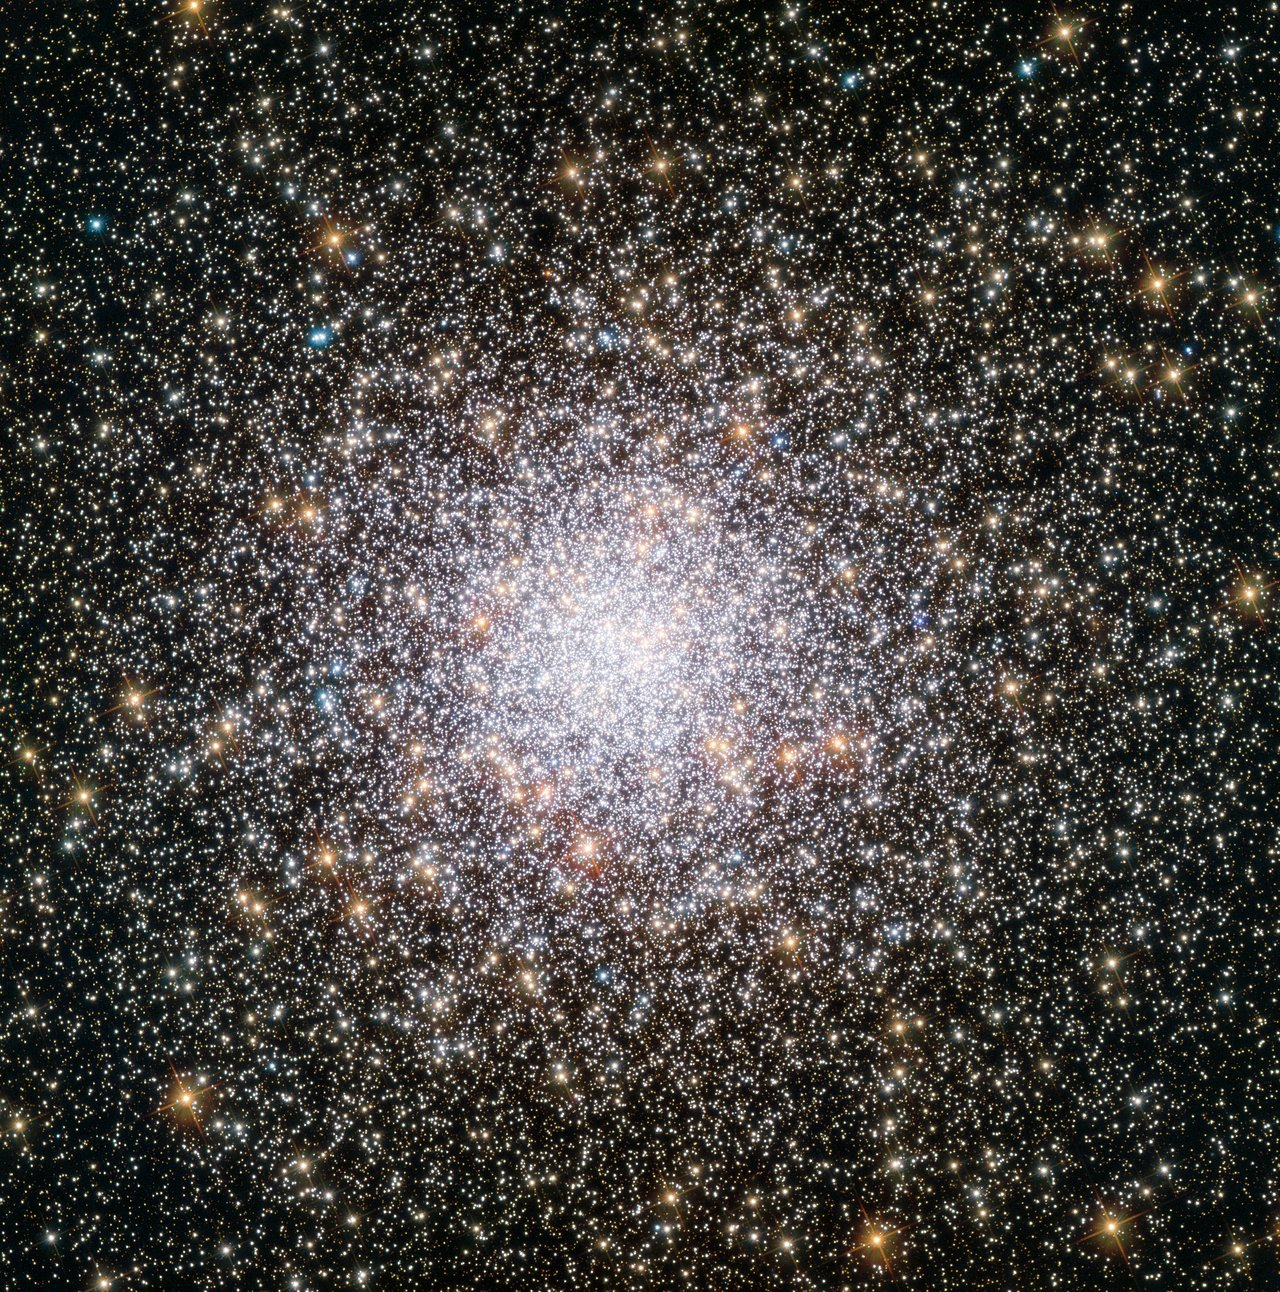
\includegraphics[scale=0.13]{media/globular_cluster_NGC362.jpg}}
\textcolor{yellow}{Her ser vi en kulehop NGC362. Det er omkring 150 kjente av disse som går i bane rundt Melkeveien. De er et flott skue også i et lite amatørteleskop.}\hyperlink{msfit7}{\pagebutton{Neste side}}\\
{\footnotesize\textcolor{yellow}{Bilde: ESA/Hubble\& NASA}}
\end{frame}
}

\begin{frame}
\label{msfit7}
\lastpagebutton{feil_msfit6}
Siden stjernene i slike hoper er født omtrent samtidig, blir de brukt til å studere stjerners livsløp da du som regel vil finne stjerner på alle mulige forskjellige stadier i livsløpet. Et viktig redskap for å studere en slik hop er {\bf HR-diagrammet}. Her ser du et slikt:
\centerline{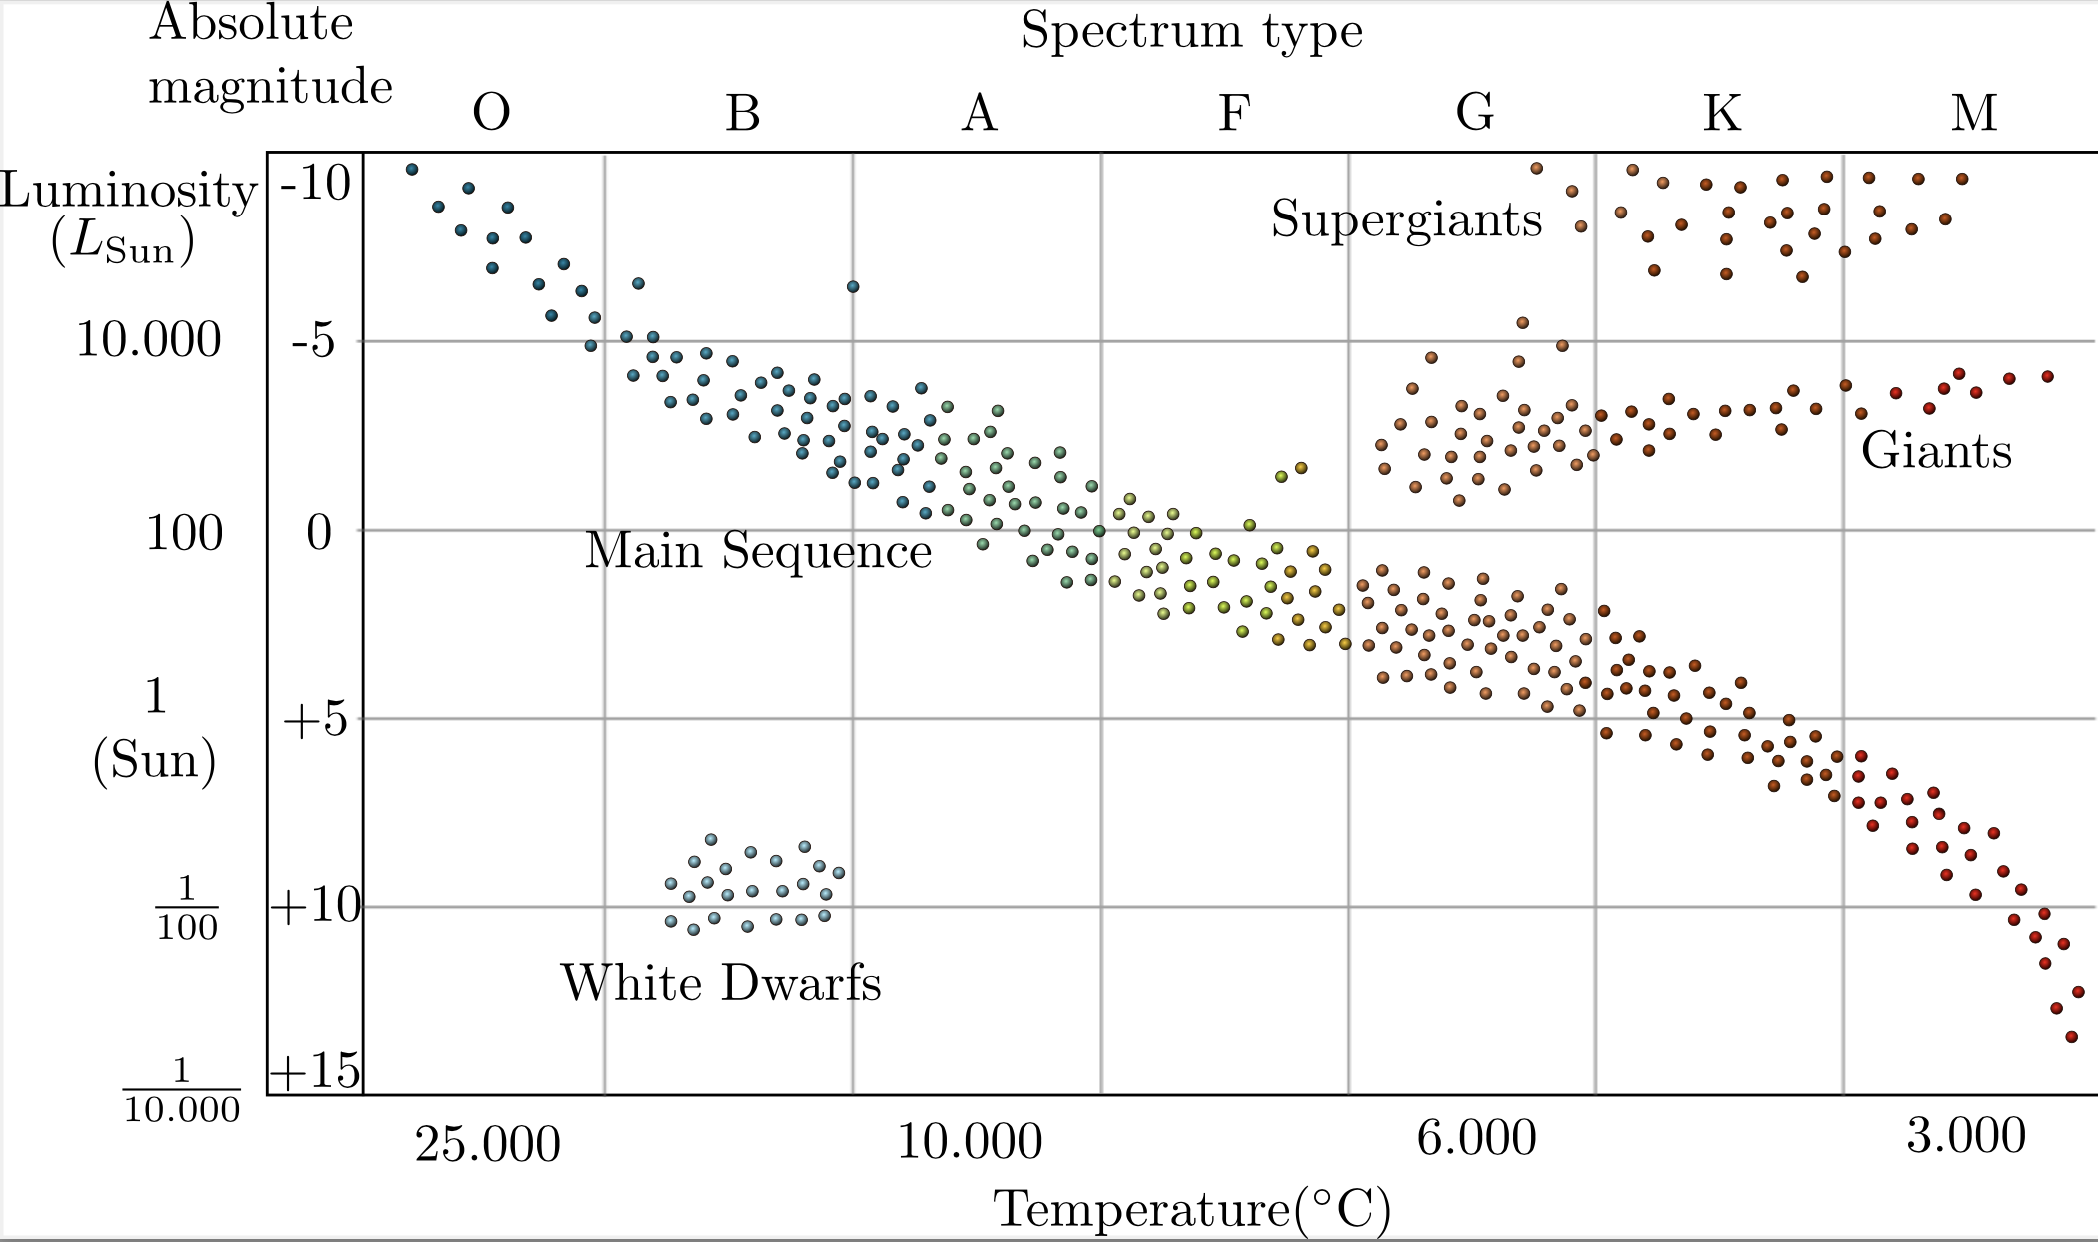
\includegraphics[scale=0.4]{media/fig_11-3.png}}
På x-aksen har vi altså stjernas overflatetemperatur, økende mot venstre. På y-aksen har vi stjernas luminositet eller absolutt størrelseklasse. For å lage et slikt diagram for en stjernehop, må du altså finne temperaturen og luminositeten til alle stjernene og plotte de inn her.
\hyperlink{msfit8}{\pagebutton{Neste side}}
\end{frame}

\begin{frame}
\label{msfit8}
\lastpagebutton{msfit7}
\centerline{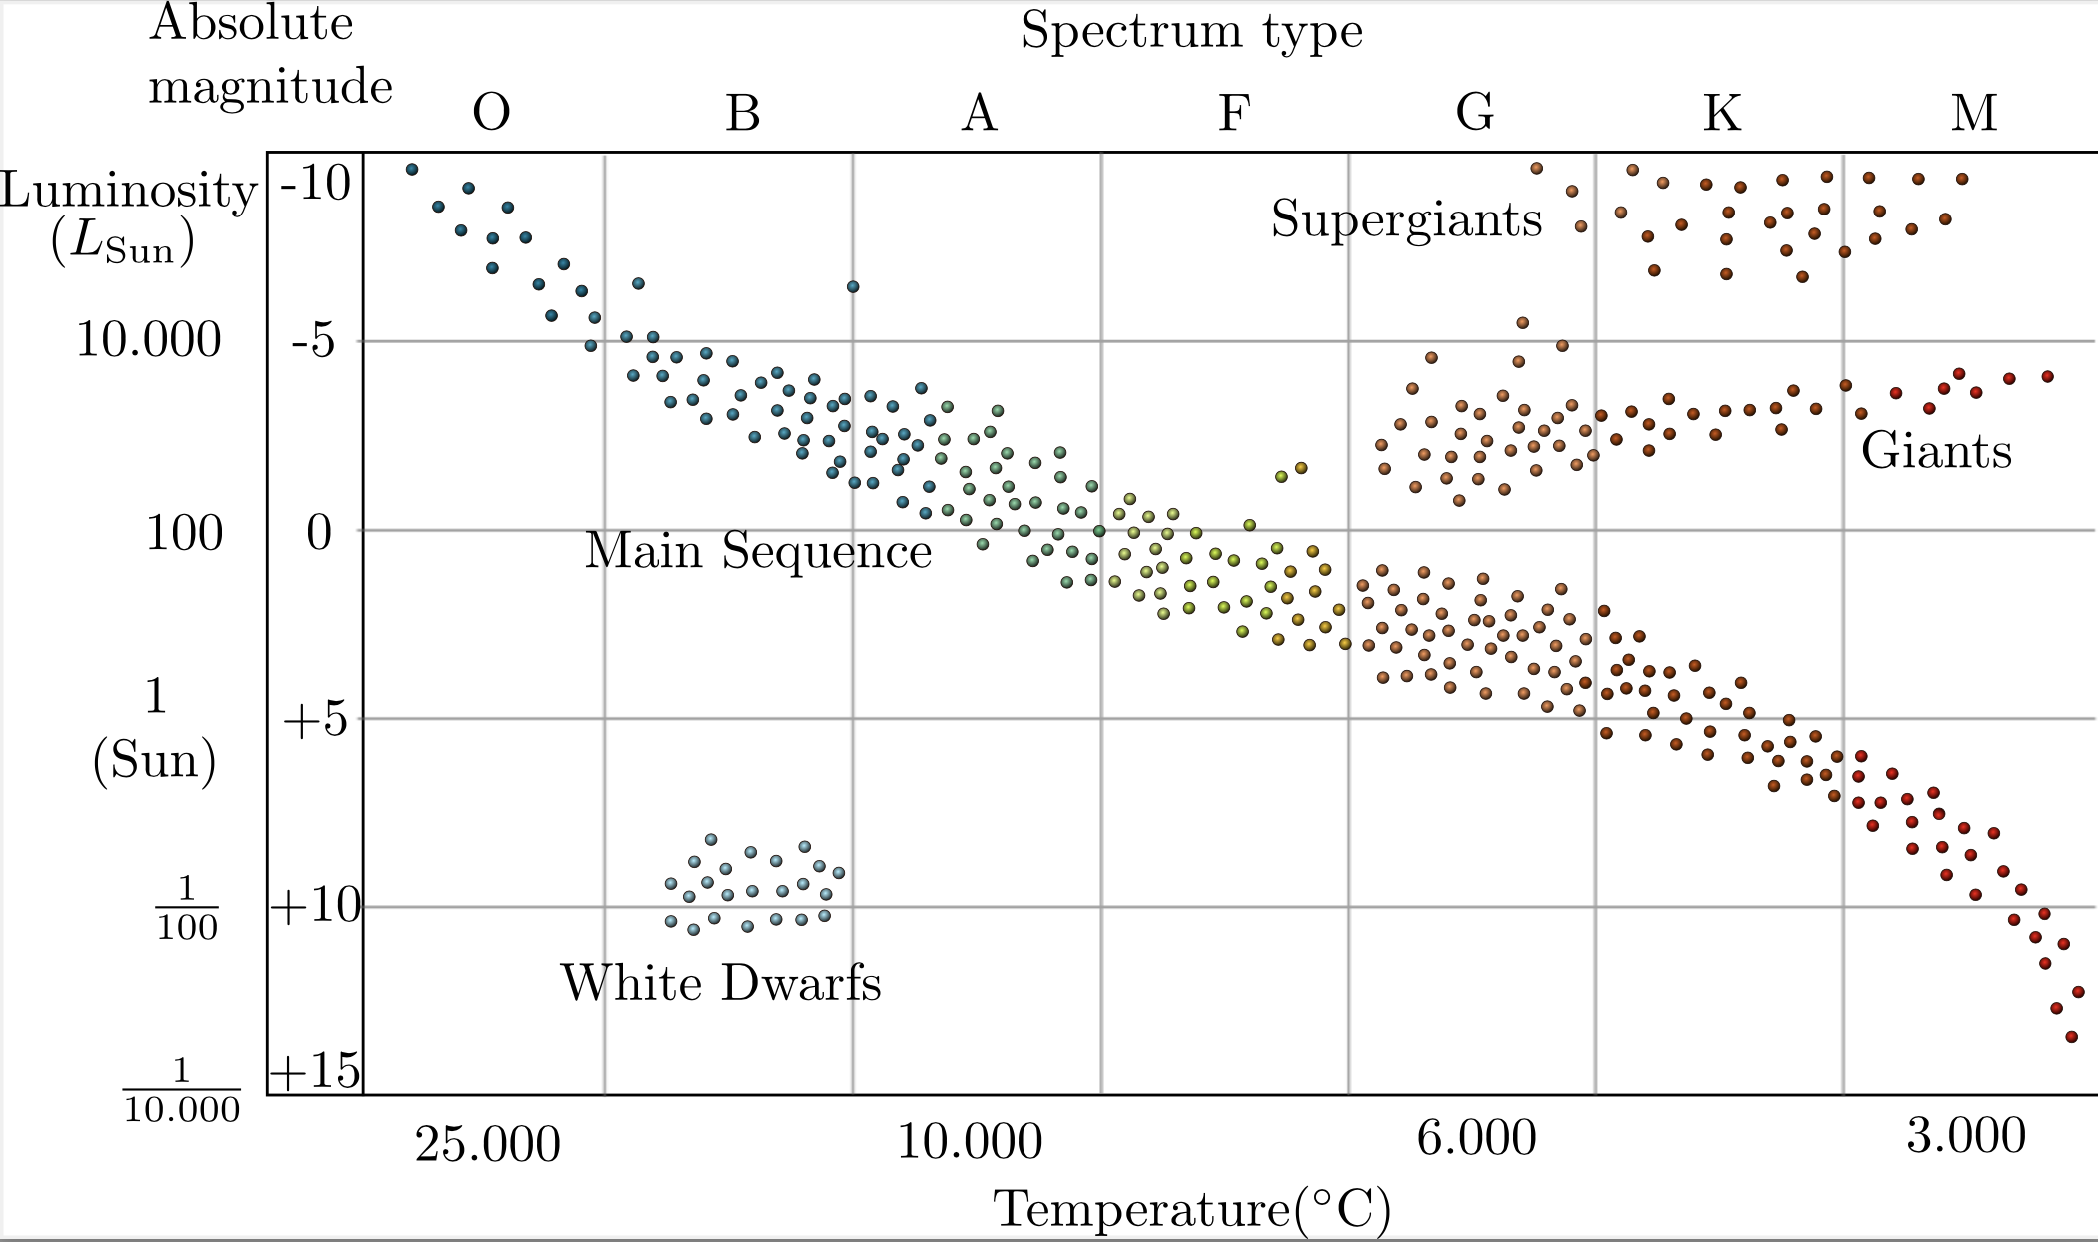
\includegraphics[scale=0.4]{media/fig_11-3.png}}
{\small
Når du gjør dette for en stjernehop vil du få et HR-diagram som det du ser her. De aller fleste stjernene ligger langs et bånd som går fra øverst til venstre (høy T og L) til nederst til høyre (lav T og L). Dette båndet kalles {\bf hovedserien (engelsk: main sequence)} og består av stjerner som enda fusjonerer hydrogen i kjernen (dette kommer vi tilbake til). Når stjernene blir eldre eser de ut og blir kjempestjerner (markert øverst til høyre i diagrammet, lav T og høy L). Til slutt vil stjerner med lav masse dø og bli til hvite dverger (nederst til venstre, høy T, lav L). \textcolor{red}{Det vi skal interessere oss for i del 3A er hovedserien}.
}
\hyperlink{msfit9}{\pagebutton{Neste side}}
\end{frame}

\begin{frame}
\label{msfit9}
\lastpagebutton{msfit8}
\centerline{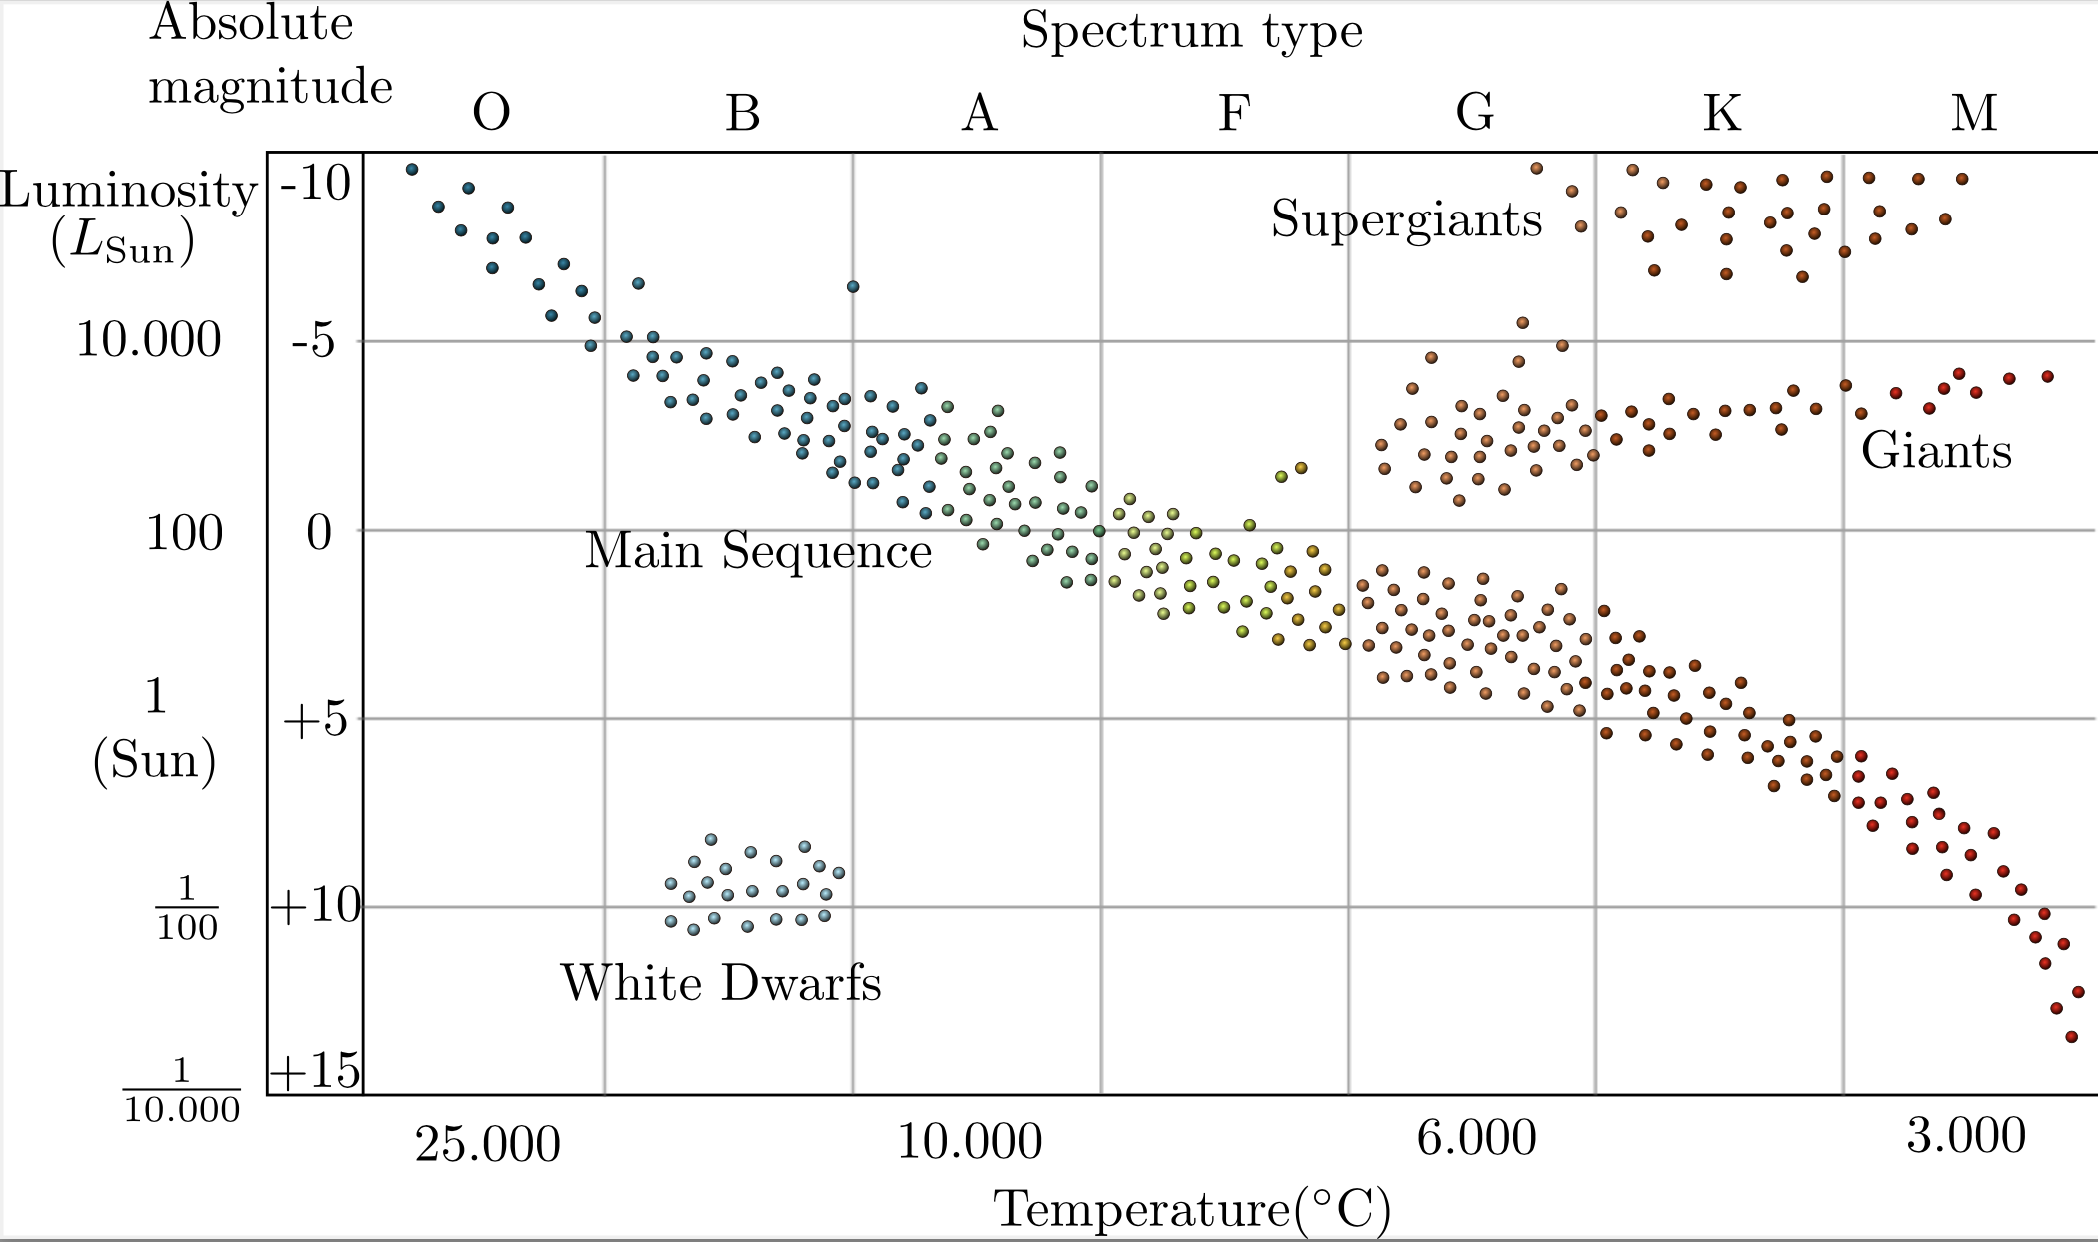
\includegraphics[scale=0.38]{media/fig_11-3.png}}
{\footnotesize
{\bf Men hvordan har man fått laget dette diagrammet?} Overflatetemperaturen er vel ikke så vanskelig, her kan man f.eks. bruke Wiens forskyvningslov (husker du?) {\bf Men hva med luminositeten??}. Vel, luminositet og absolutt størrelseklasse var jo bare to forskjellige enheter å måle samme fysiske størrelse med, kjenner du en kan du regne ut den andre. Vi hadde en sammenheng:
\[
m-M=5\log{\frac{r}{10\mathrm{pc}}}
\]
Altså: kjenner du tilsynelatende størrelseklasse $m$ (det gjør du alltid så lenge du kan observere objektet) og avstand $r$, kan du finne absolutt størrelseklasse $M$ og dermed luminositeten.
}
\hyperlink{msfit10}{\pagebutton{Neste side}}
\end{frame}

\begin{frame}
\label{msfit10}
\lastpagebutton{msfit9}
\centerline{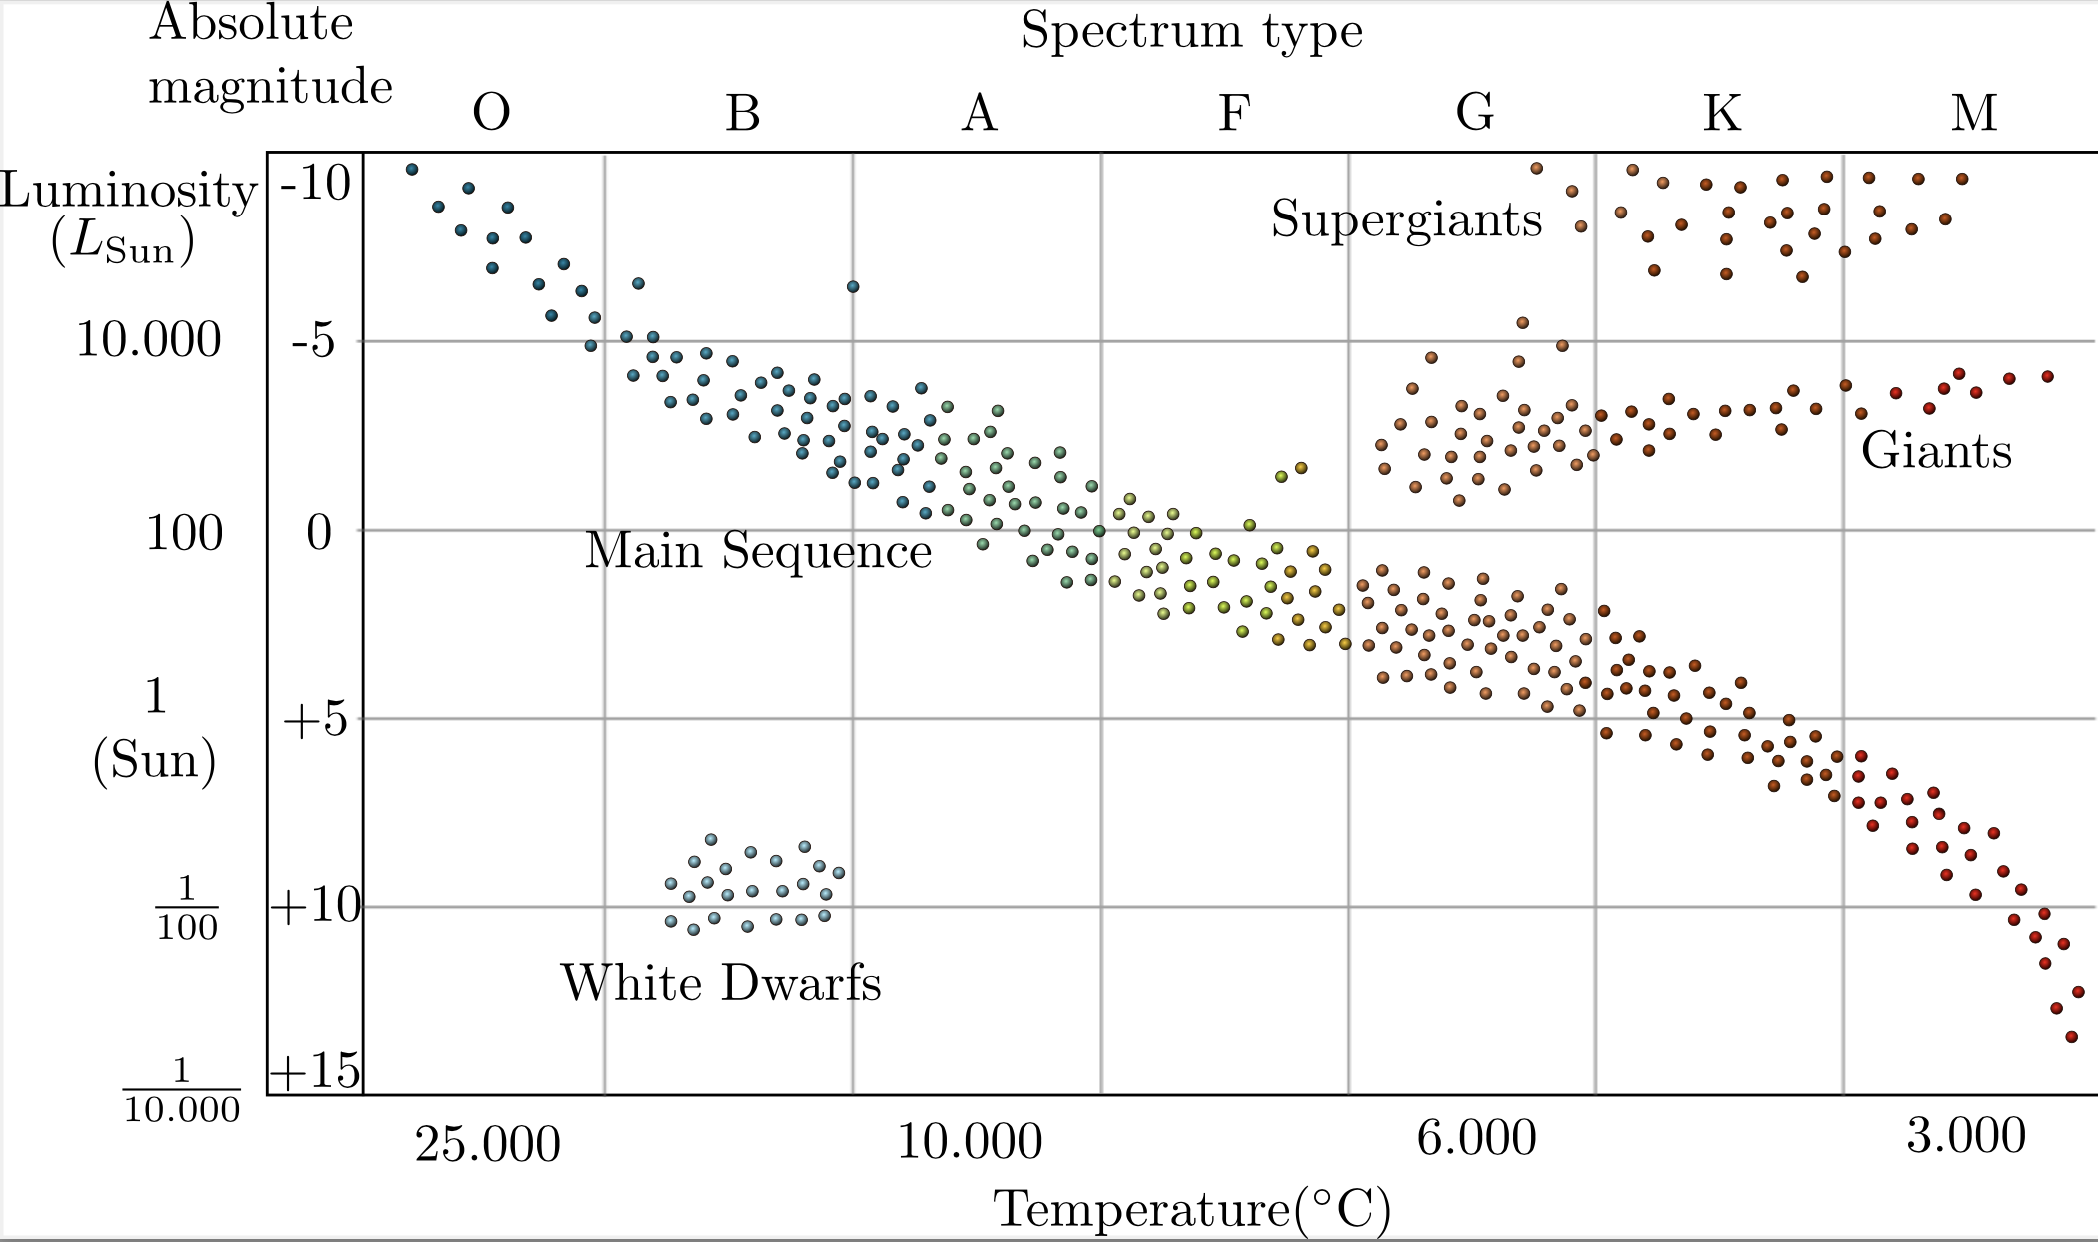
\includegraphics[scale=0.38]{media/fig_11-3.png}}
Stjernene i hopen ligger veldig tett sammen. {\bf Avstanden mellom stjernene er forsvinnende liten i forhold til avstanden fra oss til hopen.} Kjenner vi avstanden til hopen, så er det en \textcolor{red}{god antakelse å si at alle stjernene i hopen har samme avstand $r$ fra oss.} Hvis vi da f.eks. måler avstanden til hopen med {\bf parallaksemetoden}, så har vi alt vi trenger for å lage oss et slikt diagram! {\bf Har du nå klart for deg hvordan du kunne gå frem for å lage et slikt diagram?} Hvis ikke, gå gjennom de forrige sidene en gang til og spør hvis noe er uklart.
\hyperlink{msfit11}{\pagebutton{Jeg forstår og er klar for neste side}}
\end{frame}


\begin{frame}
\label{msfit11}
\lastpagebutton{msfit10}
\centerline{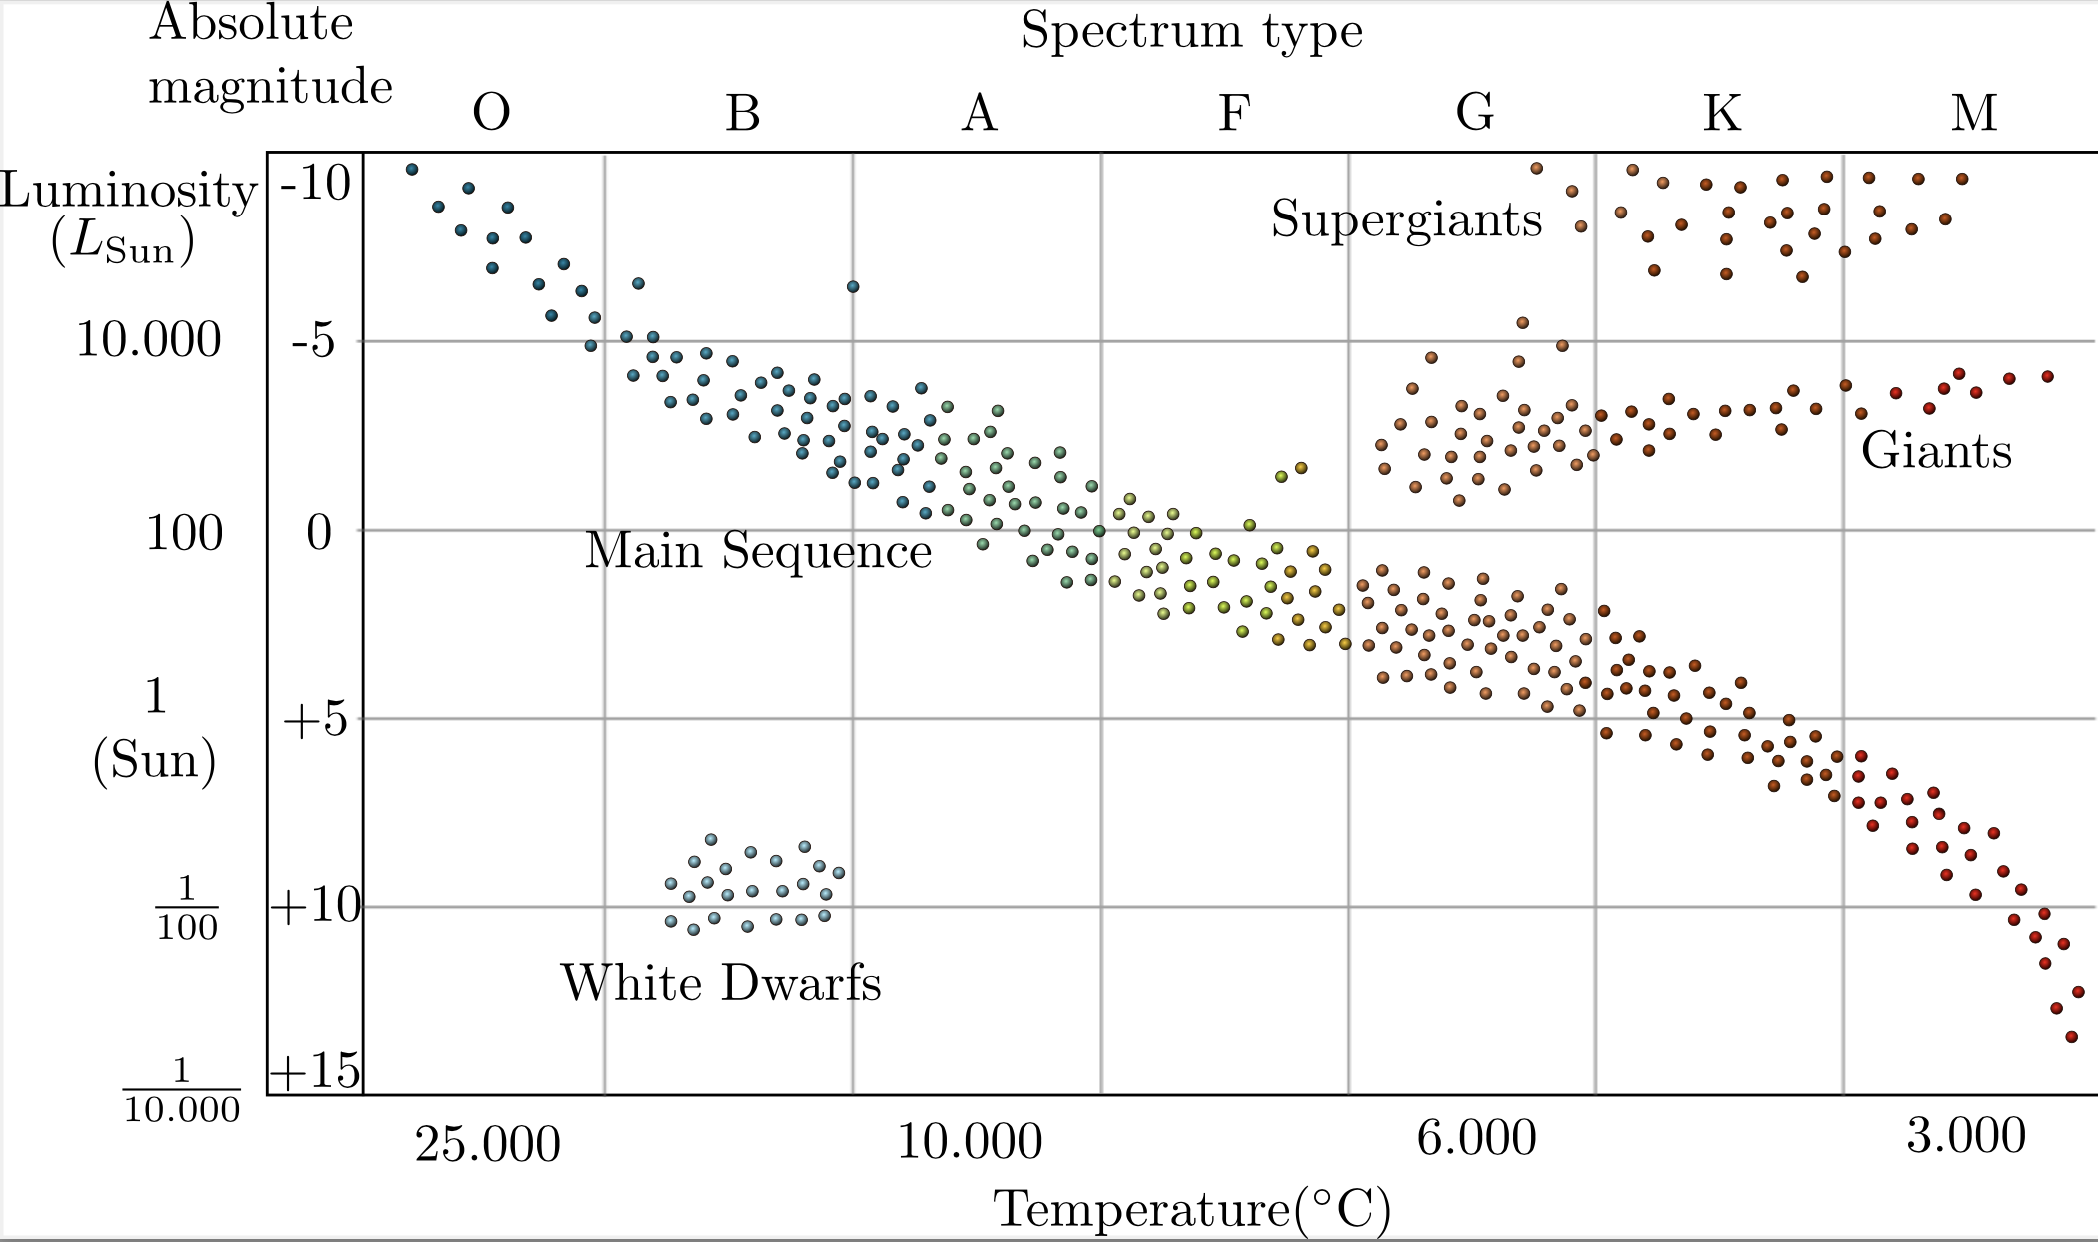
\includegraphics[scale=0.38]{media/fig_11-3.png}}
De fysiske prosessene som danner stjerner er alltid de samme, og vil være den samme for alle hoper. Fordelingen av stjerner i HR-diagrammet forventer vi derfor vil være ganske lik mellom hopene. Dette er bekreftet av observasjoner av mange forskjellige hoper. Vi får alltid et HR-diagram, og da spesielt en hovedserie, som er akkurat slik som på denne figuren med samme forhold mellom $L$ og $T$ for hovedseriestjernene.
\hyperlink{feil_msfit12}{\pagebutton{Neste side}}
\end{frame}


{
\setbeamercolor{background canvas}{bg=black}
\begin{frame}
\label{feil_msfit12}
\lastpagebutton{msfit11}
\centerline{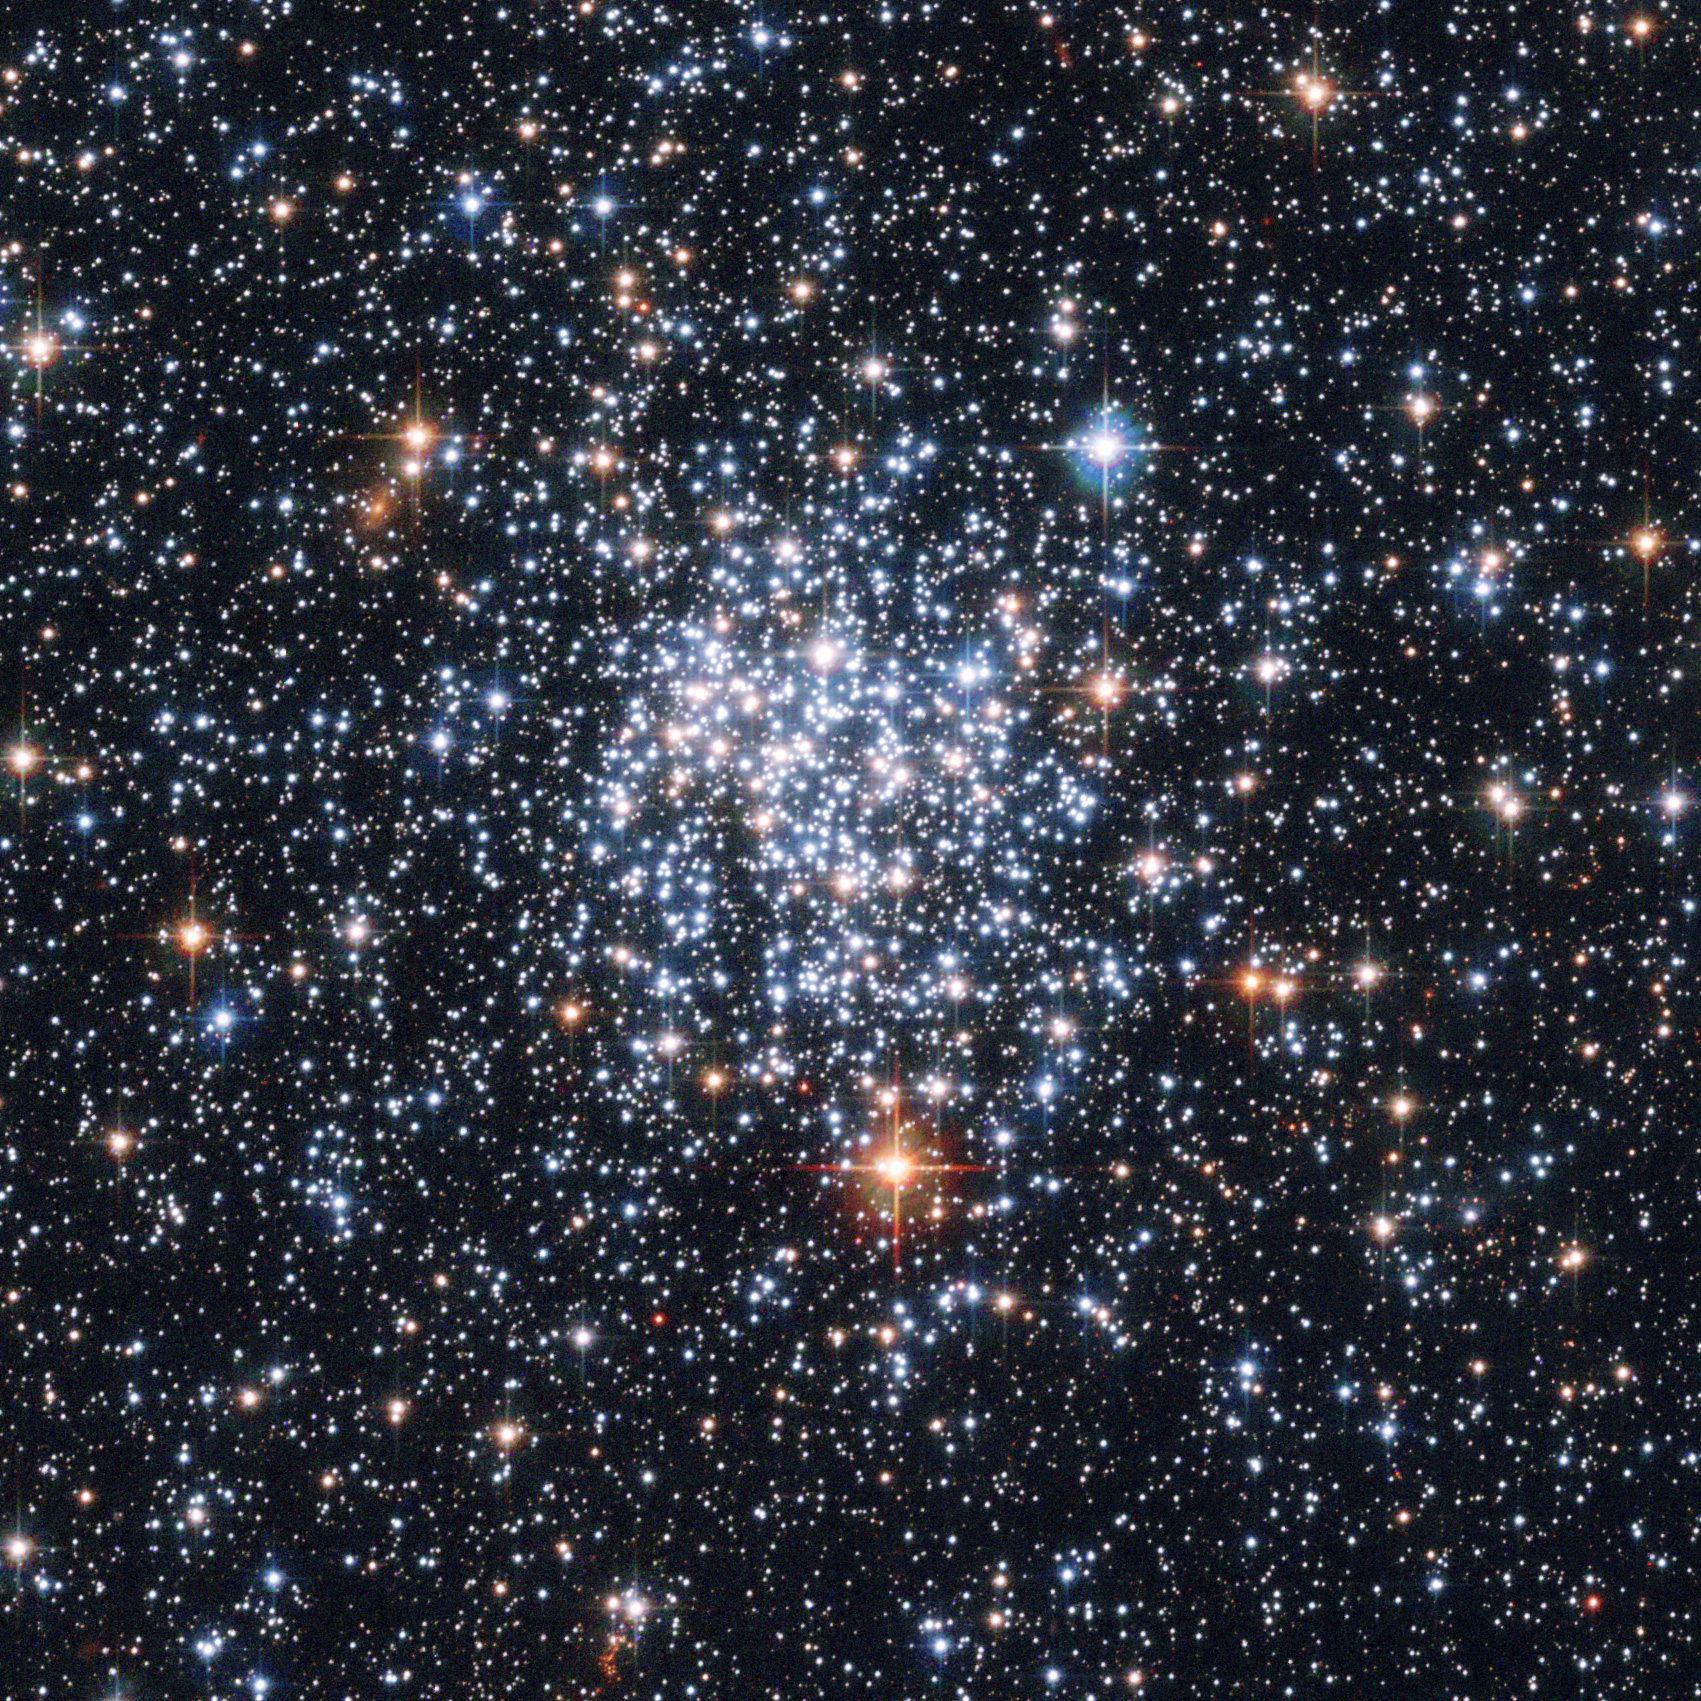
\includegraphics[scale=0.09]{media/open_cluster_NGC265.jpg}}
\textcolor{yellow}{Hva nå med vår åpne hop NGC265 som ligger i den Store Magellanske Sky? Den ligger for langt unna til at vi kan måle avstanden med parallakse! Vi kan altså kun måle {\bf tilsynelatende størrelseklasse} $m$ og {\bf ikke absolutt størrelseklasse} $M$ for stjernene i denne hopen. Overflatetemperaturen kan vi enda måle, da vi kun trenger spektret fra stjernen for å måle den.}
\hyperlink{msfit13}{\pagebutton{Neste side}}
\end{frame}
}

\begin{frame}
\label{msfit13}
\lastpagebutton{feil_msfit12}
\centerline{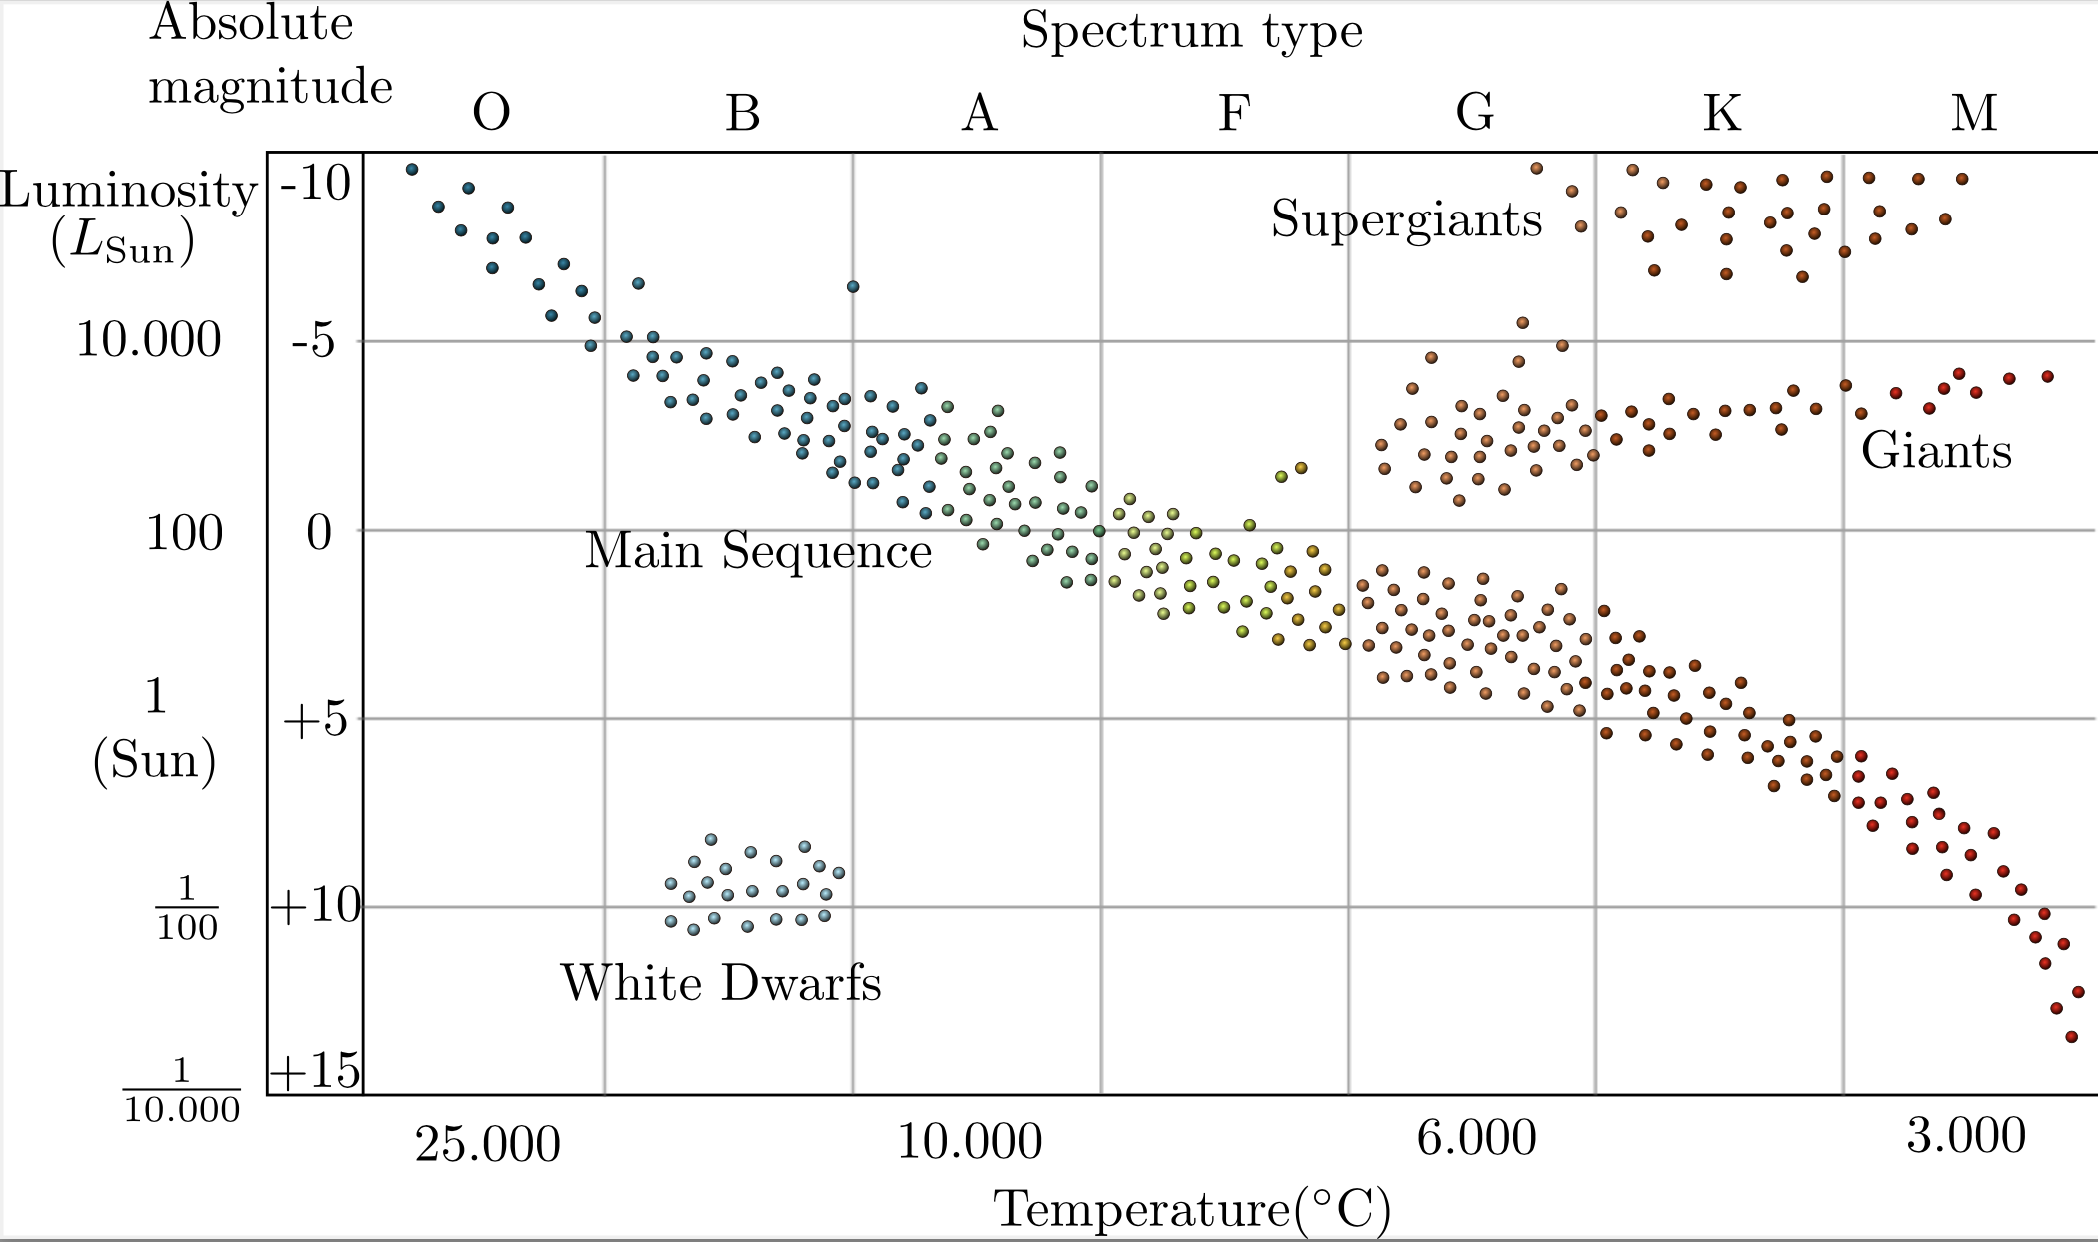
\includegraphics[scale=0.38]{media/fig_11-3.png}}
Dermed kunne vi jo forsøke å lage oss et HR-diagram som det over, men med $m$ istedenfor $M$ på y-aksen. Da vil vi ikke lenger ha luminositet på y-aksen. Men hvordan vil dette HR-diagrammet se ut? Hva vil være forskjellen med det vanlige HR-diagrammet som har absolutt størrelseklasse og dermed $M$ på y-aksen?
\hyperlink{red_msfit14}{\pagebutton{Tenk det godt om før du blar om!}}
\end{frame}

{
\setbeamercolor{background canvas}{bg=red}
\begin{frame}
\label{red_msfit14}
\lastpagebutton{msfit13}
{\Large
\textcolor{yellow}{Her bør du faktisk stoppe opp og tenke litt! Gi deg noen minutter til å tenke godt gjennom problemstillingen: hvordan tror du dette diagrammet blir seende ut? Du har all kunnskap du trenger for å vite det!}
}
\hyperlink{red_msfit15}{\pagebutton{Tenk det godt om før du blar om!}}
\end{frame}
}

{
\setbeamercolor{background canvas}{bg=red}
\begin{frame}
\label{red_msfit15}
\lastpagebutton{red_msfit14}
{\Large
\textcolor{yellow}{OK da, du skal få et hint: formelen
\[
m-M=5\log{\frac{r}{10\mathrm{pc}}}
\]
gir deg svaret!}
}
\hyperlink{msfit16}{\pagebutton{Tenk det godt om før du blar om!}}
\end{frame}
}


\begin{frame}
\label{msfit16}
\lastpagebutton{red_msfit15}
La oss skrive om formelen:
\[
m=M+5\log{\frac{r}{10\mathrm{pc}}}
\]
Ser du at hvis vi nå plotter $m$ på y-aksen isteden for $M$, så blir $m$-verdien det samme som $M$-verdien pluss {\bf en konstant som er omtrent den samme for alle stjernene i hopen?}. Husk at den innbyrdes avstanden mellom stjernene i hopen er forsvinnene liten i forhold til avstanden $r$ til hopen slik at vi i praksis kan si at alle stjernene i hopen er i avstand $r$. Da blir det siste leddet konstant. {\bf Bør vi ikke da se et helt identisk HR-diagram, bare at alle stjernene er skiftet oppover eller nedover med en konstant verdi?}
\hyperlink{msfit17}{\pagebutton{Tenk det godt om før du blar om!}}
\end{frame}


\begin{frame}
\label{msfit17}
\lastpagebutton{msfit16}
{\small\bf Får vi ikke da noe slik som dette?}
%\centerline{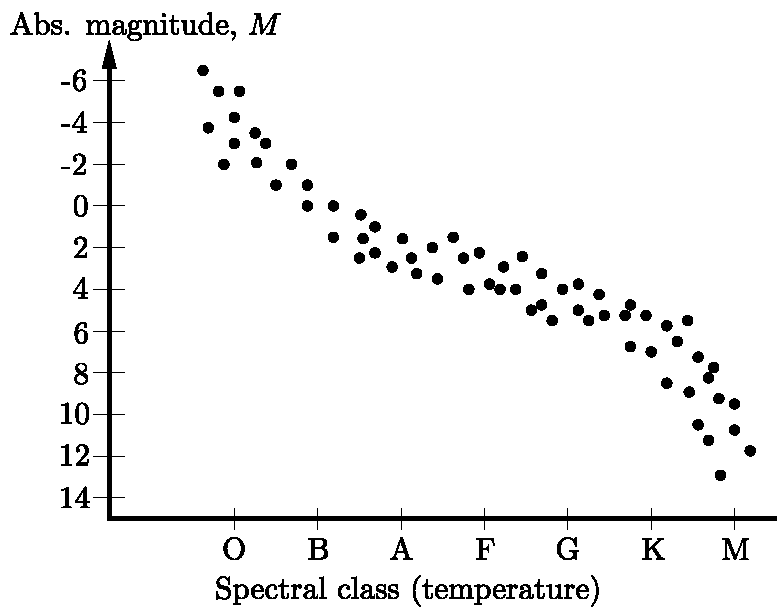
\includegraphics[scale=0.38]{media/fig_11-4a.pdf}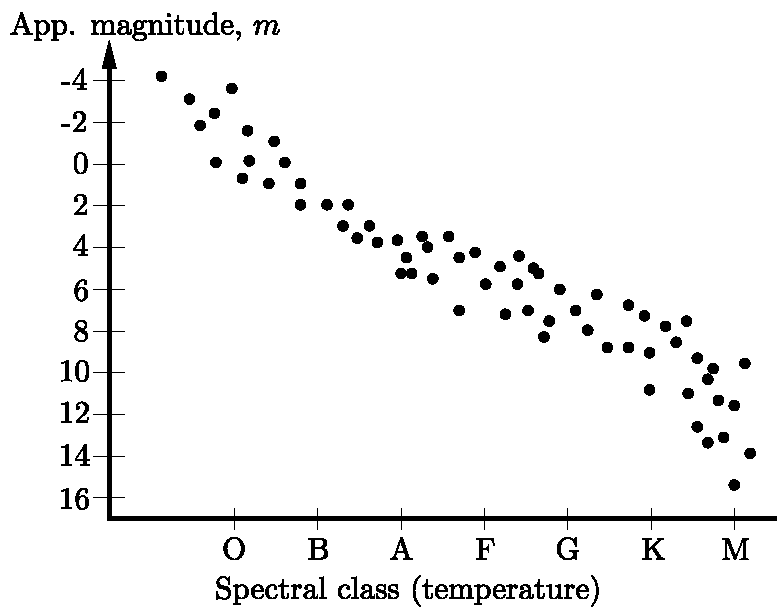
\includegraphics[scale=0.38]{media/fig_11-4b.pdf}}
\centerline{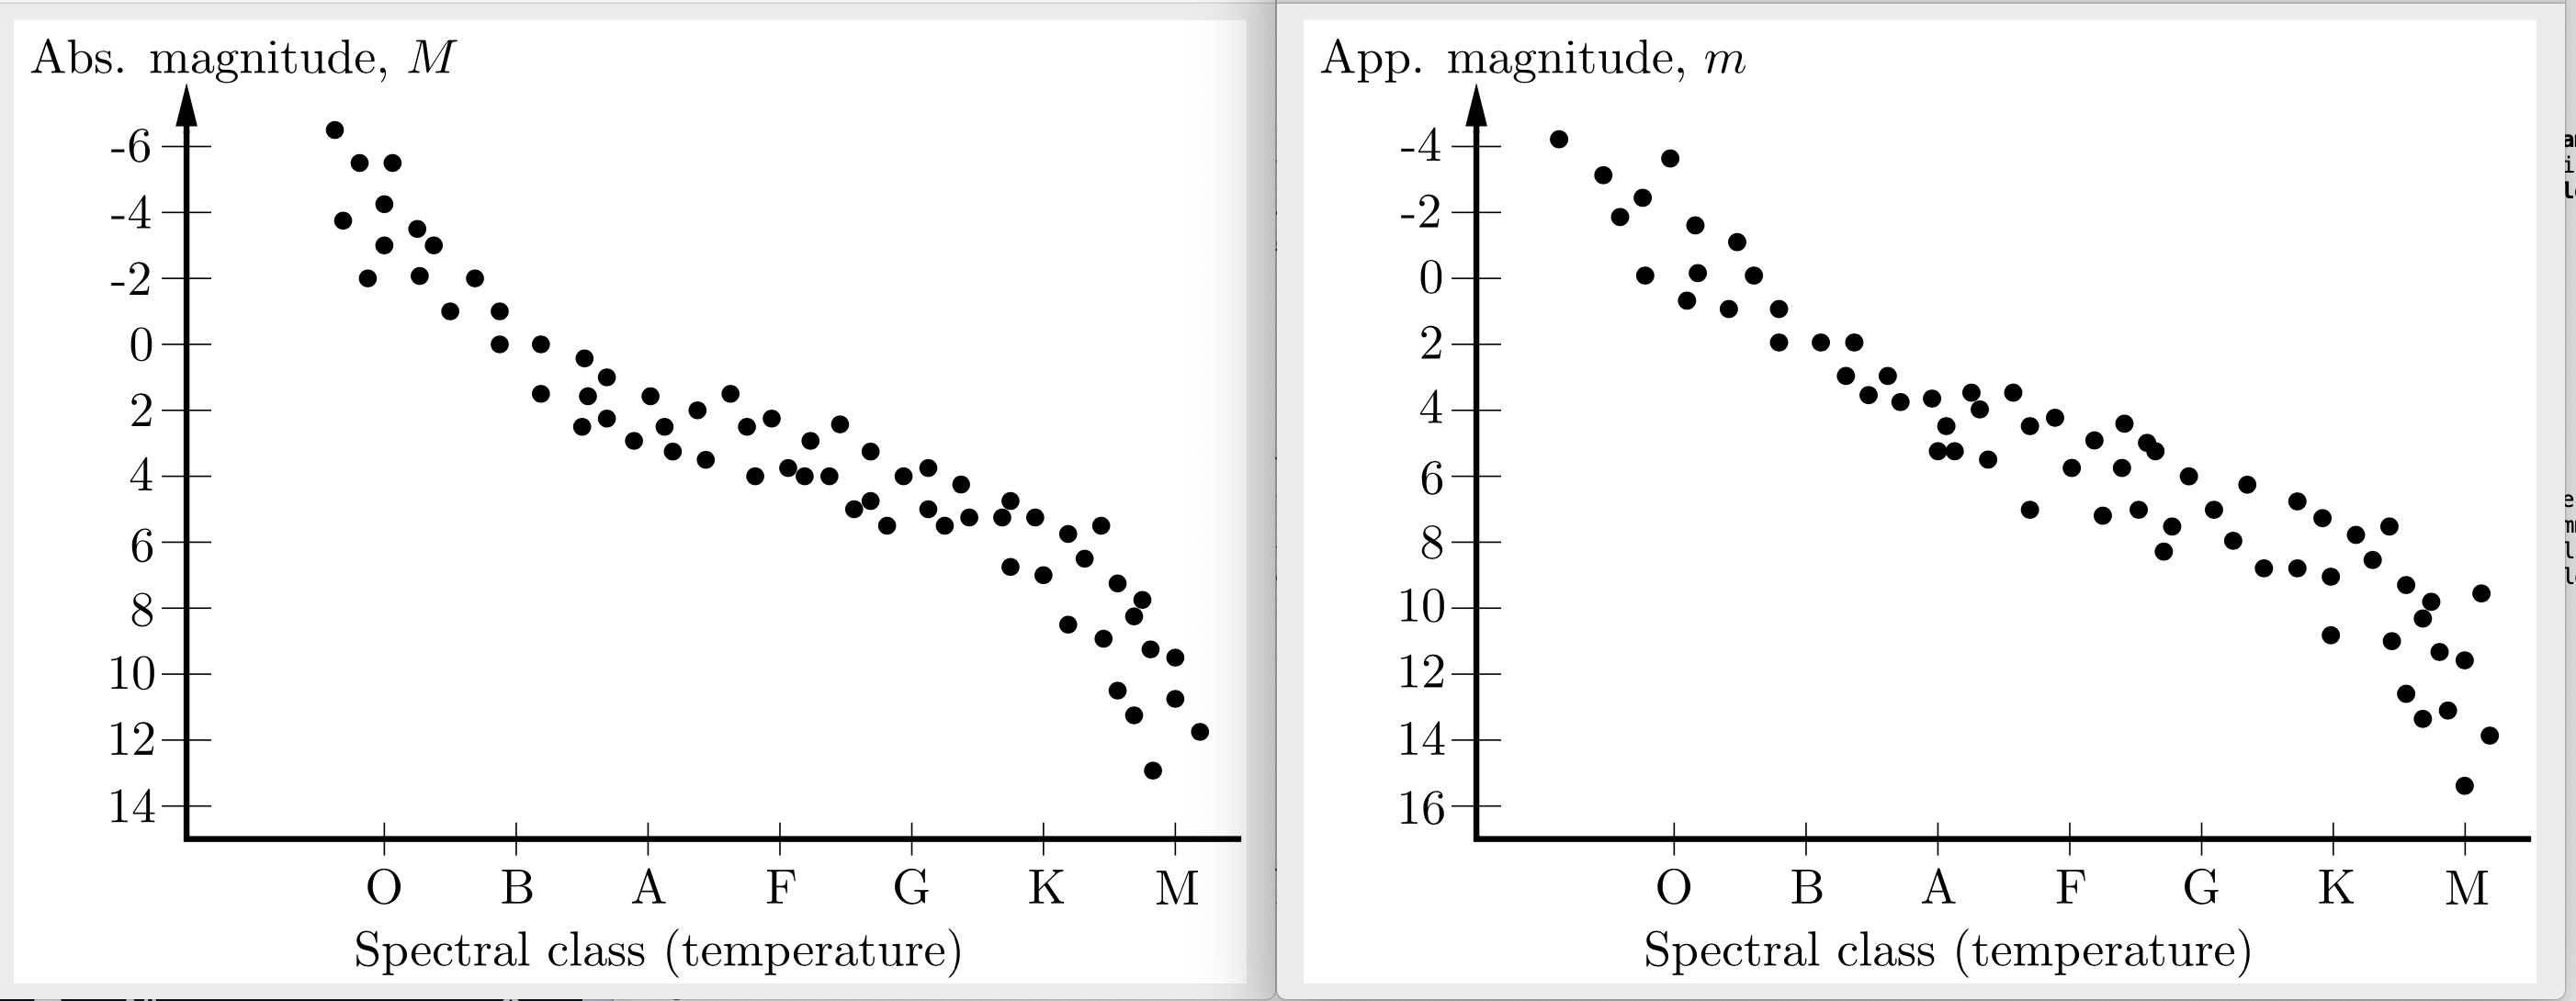
\includegraphics[scale=0.2]{media/fig_11-4comb.png}}
{\footnotesize
(ikke bry deg om teksten på x-aksen for nå, ``spektralklasse'' er omtrent det samme som temperaturen til stjernene.). Her har vi kun tegnet inn hovedserien for å gjøre det lettere å se. Diagrammet til venstre er tatt fra stjernehoper med kjent avstand og dermed kjent absolutt størrelseklasse $M$. Dette diagrammet har $M$ på y-aksen. Diagrammet til høyre derimot er tatt fra en stjernehop med ukjent avstand, og dermed ukjent absolutt størrelseklasse. Der har vi kun tilsynelatende størrelseklasse $m$ på y-aksen. Men vi vet at dette bare er skøvet opp eller ned med et konstant tall. Kan du bruke disse to diagrammene samt formelen på forrige side til å finne avstanden til stjernehopen i diagrammet til høyre?
}
\hyperlink{msfit17x}{\pagebutton{Tenk det godt om før du blar om!}}
\end{frame}



\begin{frame}
\label{msfit17x}
\lastpagebutton{msfit17}
%\centerline{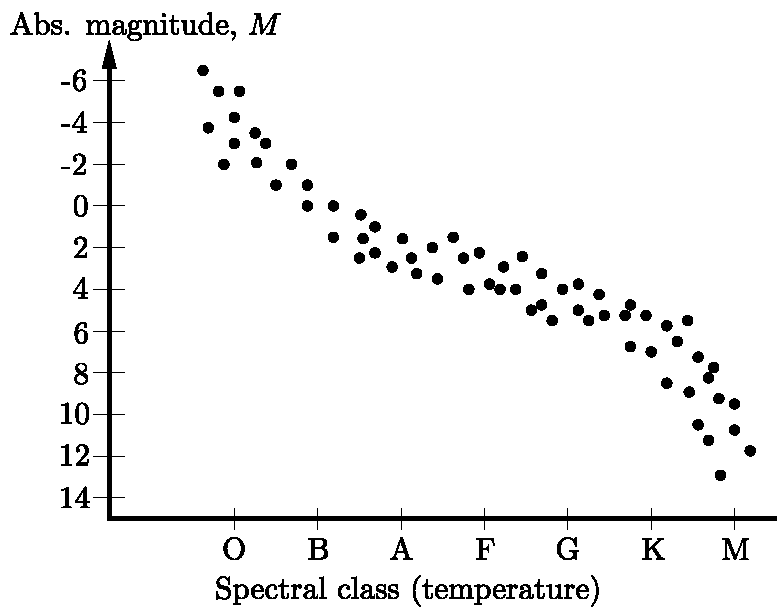
\includegraphics[scale=0.38]{media/fig_11-4a.pdf}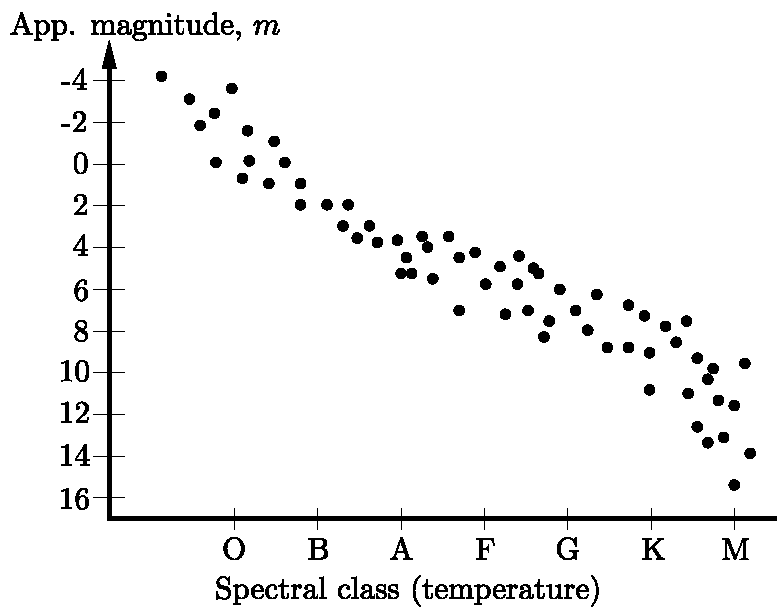
\includegraphics[scale=0.38]{media/fig_11-4b.pdf}}
\centerline{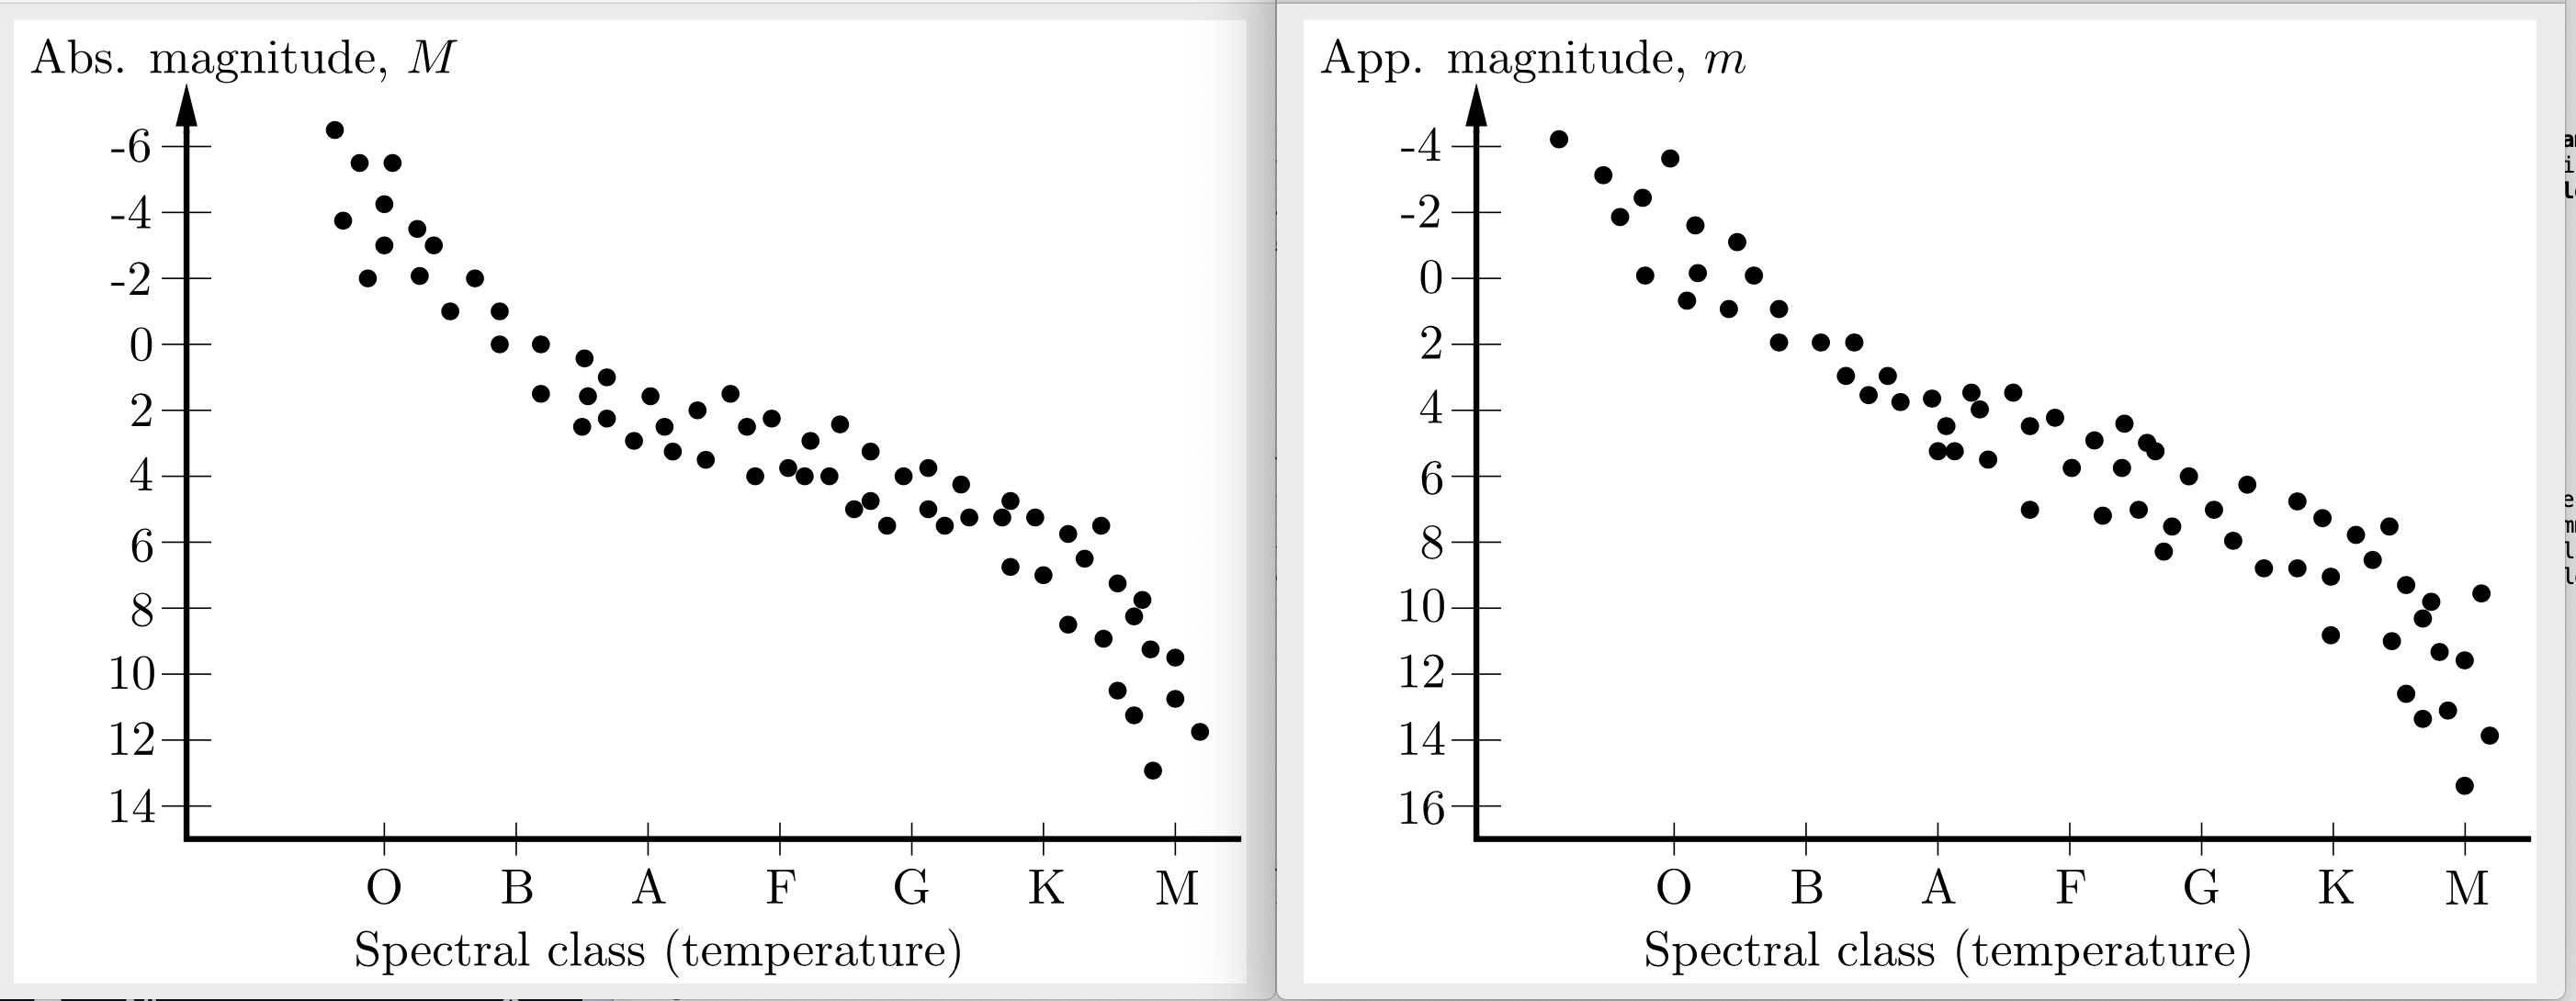
\includegraphics[scale=0.2]{media/fig_11-4comb.png}}
{\Large For det første: er hopen til høyre nærmere eller lenger vekk enn 10pc? (og hvordan kan du se det uten noe regning?)}
\hyperlink{msfit17a}{\choicebutton{nærmere}}\ \ \ \hyperlink{msfit17b}{\choicebutton{lenger vekk}}
\end{frame}

\begin{frame}
\label{msfit17a}
\lastpagebutton{msfit17x}
%\centerline{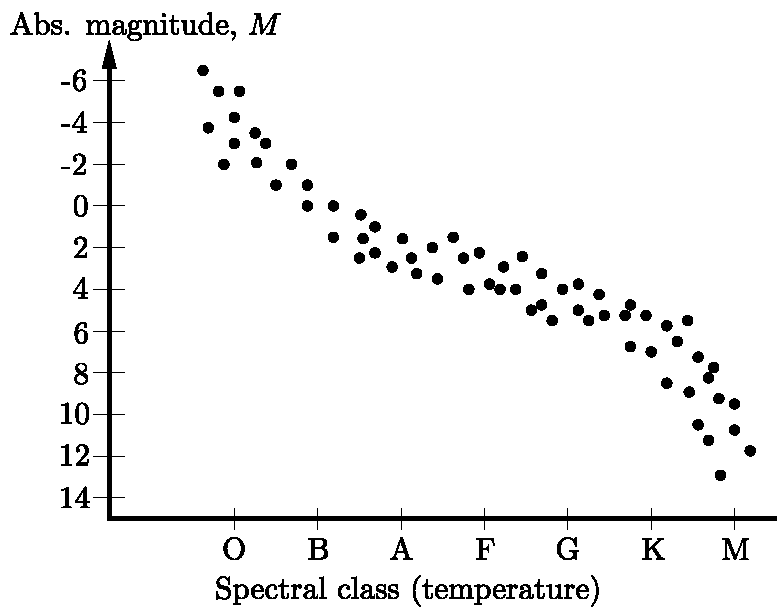
\includegraphics[scale=0.38]{media/fig_11-4a.pdf}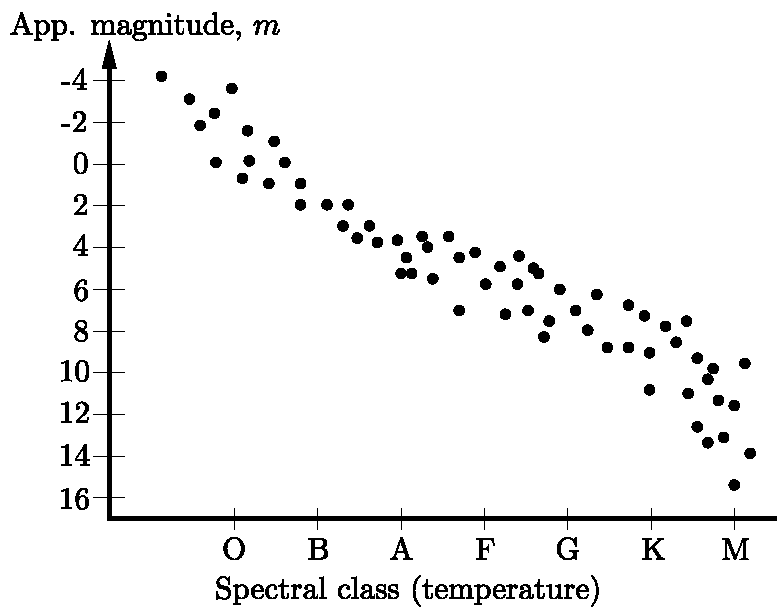
\includegraphics[scale=0.38]{media/fig_11-4b.pdf}}
\centerline{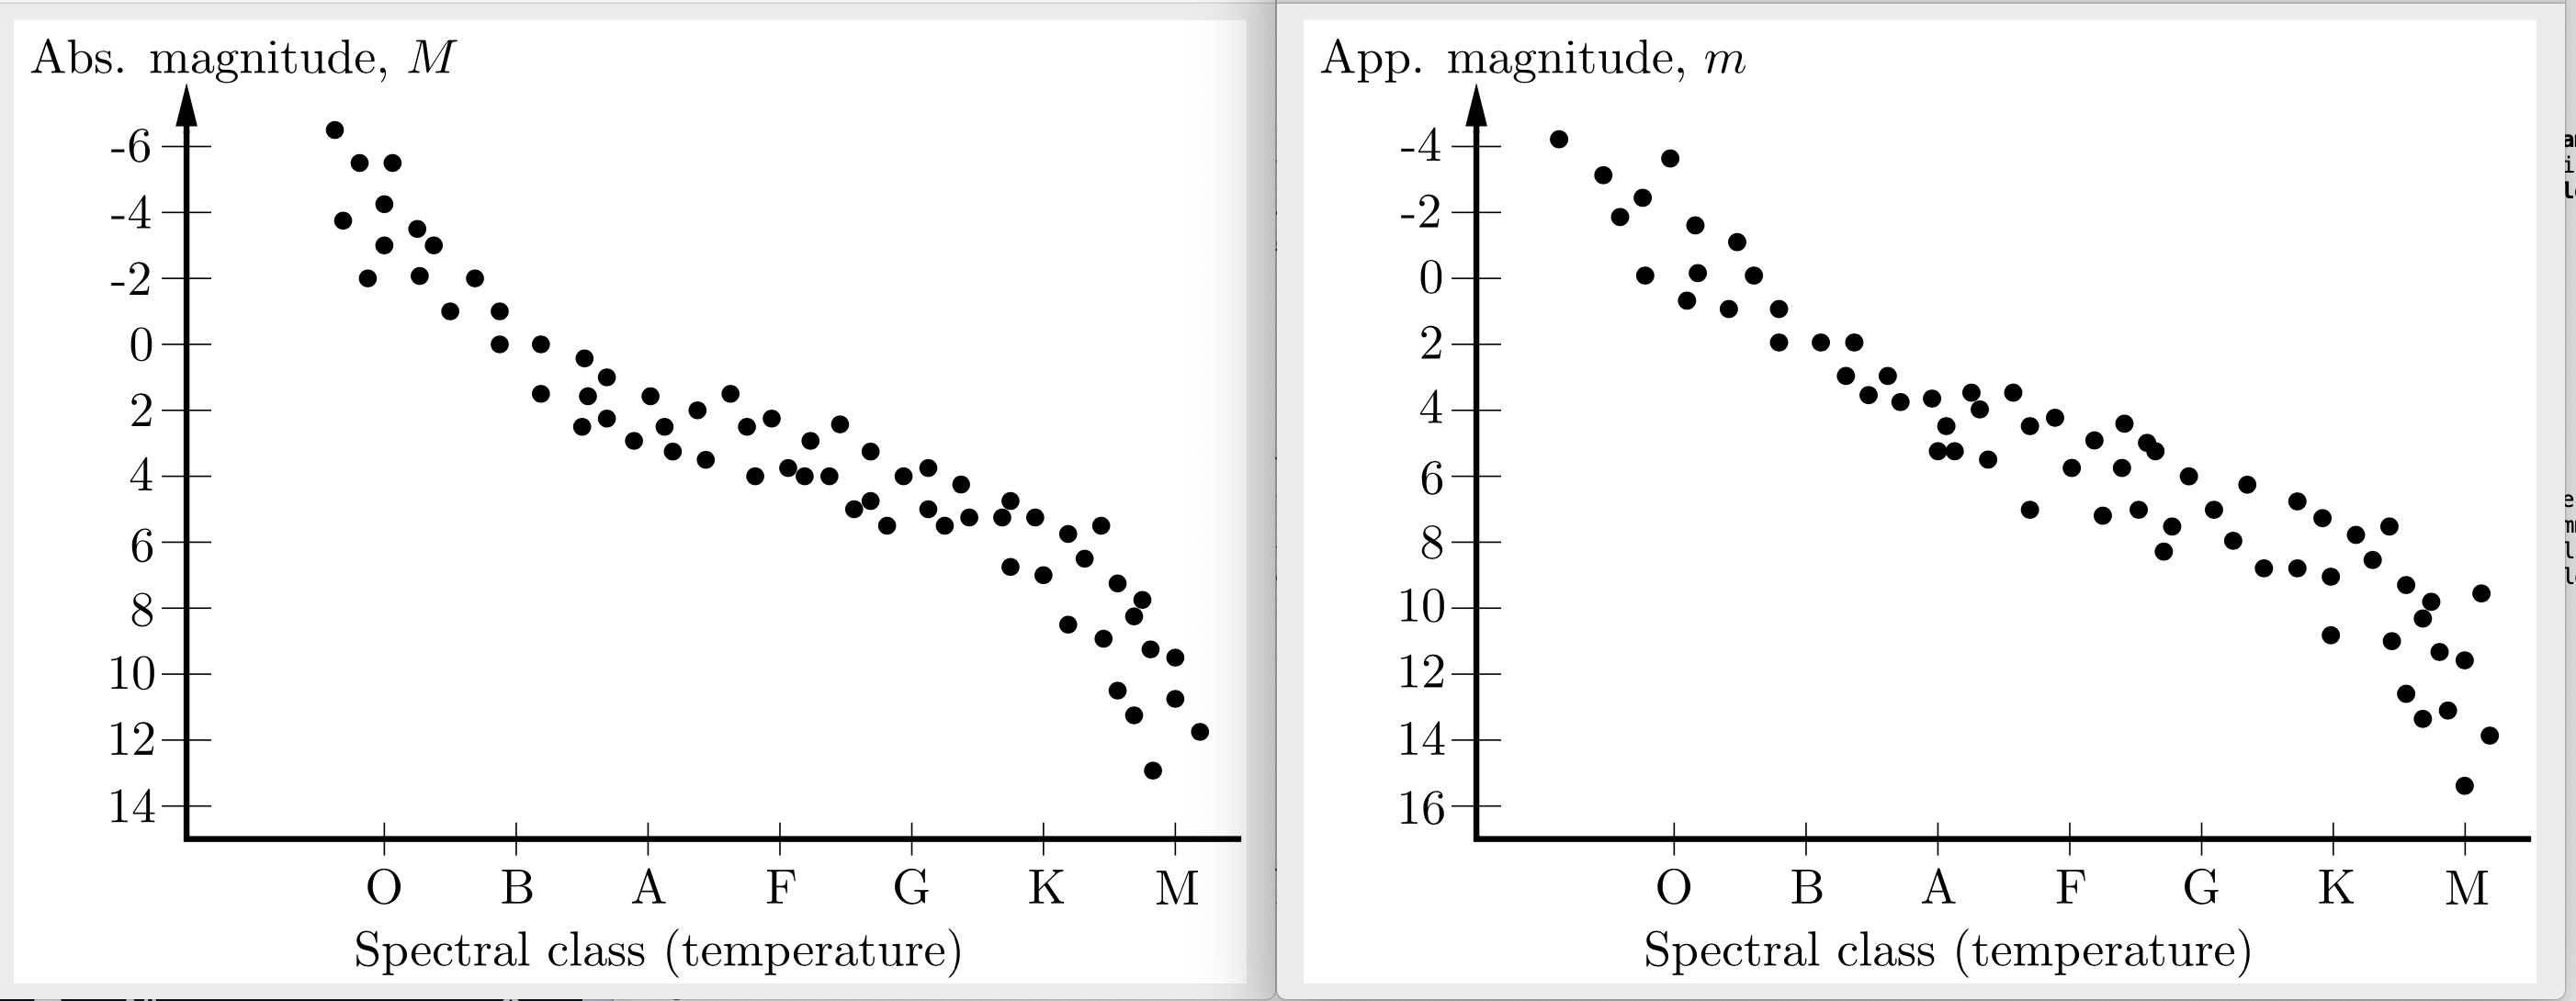
\includegraphics[scale=0.2]{media/fig_11-4comb.png}}
{\Large Det ble nok galt! Vi vet at de absolutte størrelseklassene i en stjernehop er fordelt som på figuren til venstre. Er den tilsynelatende størrelseklassen for stjernene i hopen til høyre større eller mindre enn den absolutte? Og betyr større eller mindre tilsyndelatende størrelseklasse at stjernene er lettere eller vanskeligere å se på himmelen?}
\hyperlink{msfit17b}{\pagebutton{Jeg har tenkt meg litt om nå...}}
\end{frame}

\begin{frame}
\label{msfit17b}
\lastpagebutton{msfit17x}
%\centerline{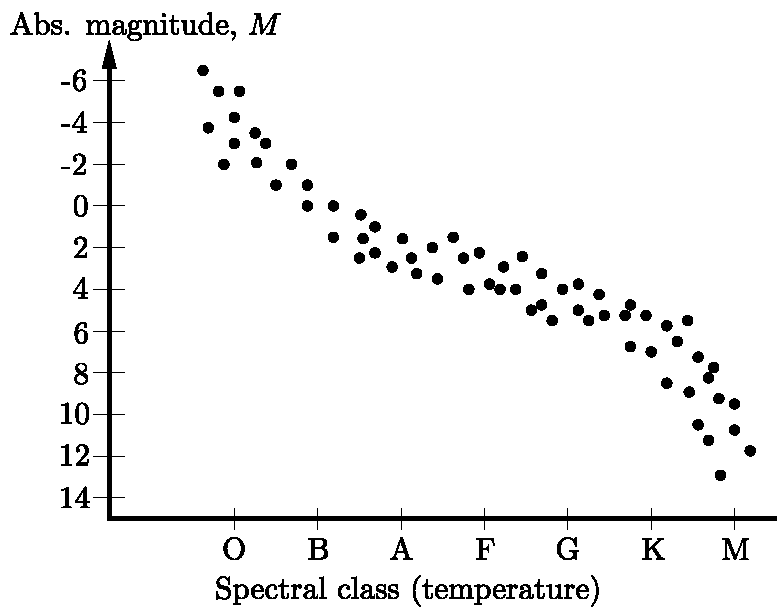
\includegraphics[scale=0.38]{media/fig_11-4a.pdf}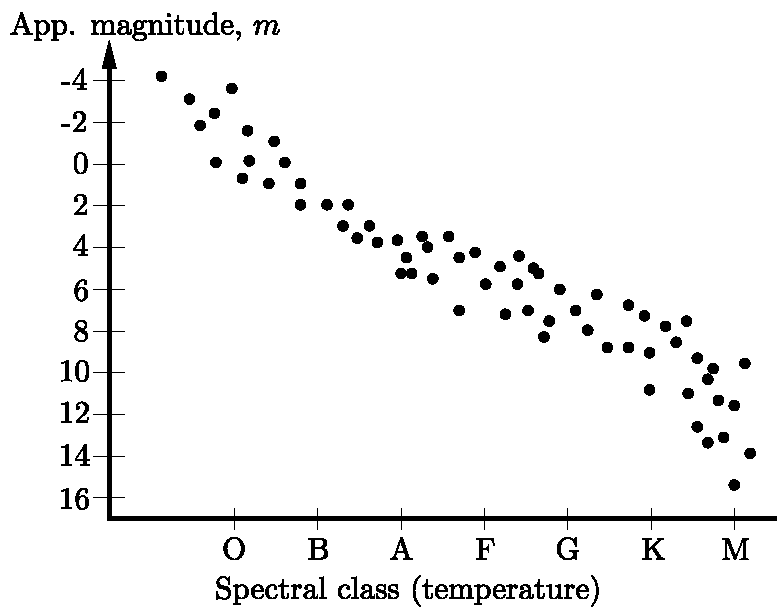
\includegraphics[scale=0.38]{media/fig_11-4b.pdf}}
\centerline{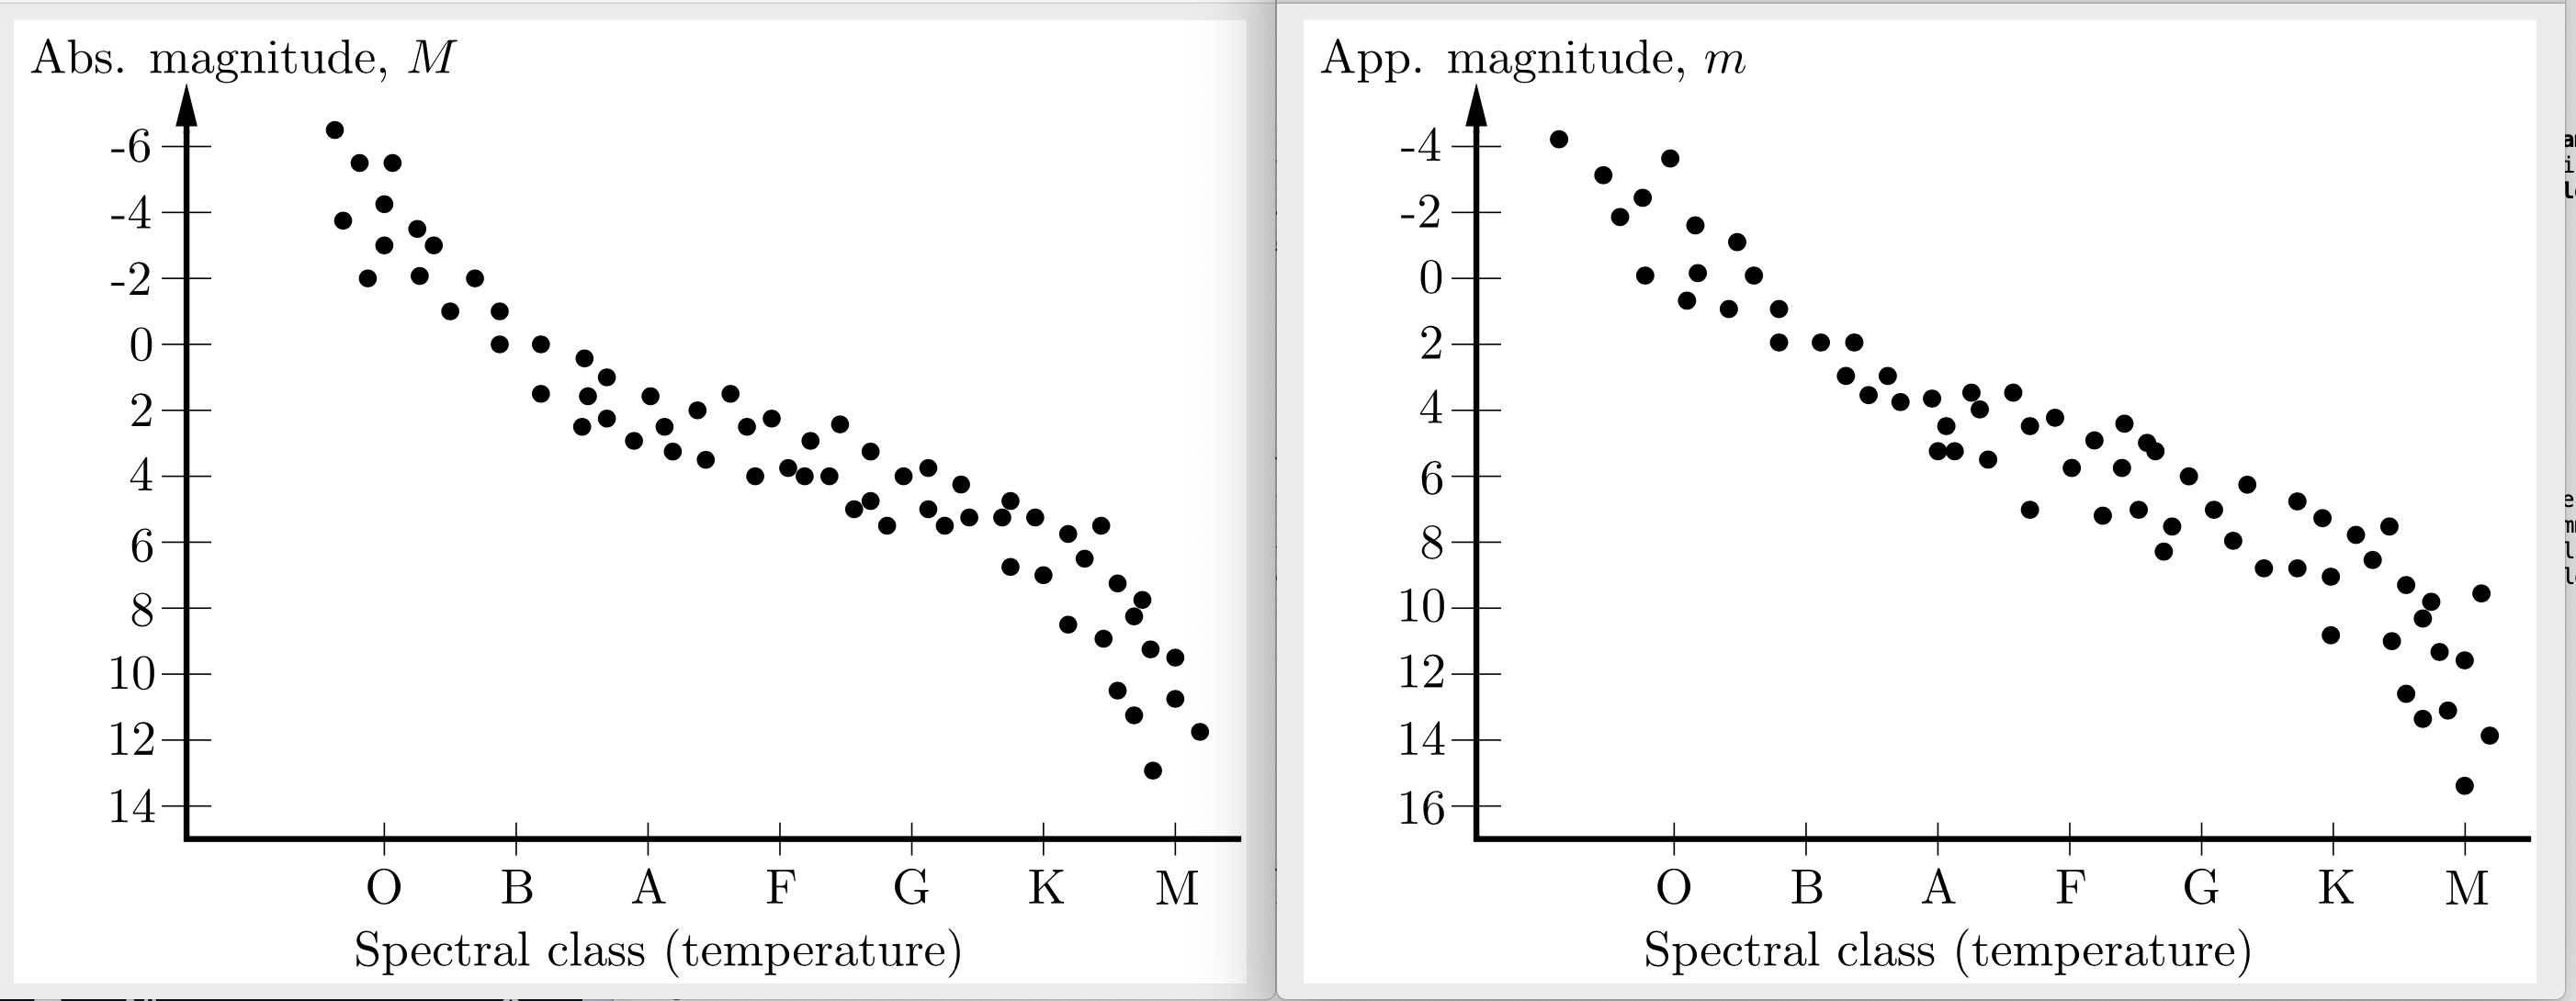
\includegraphics[scale=0.2]{media/fig_11-4comb.png}}
{\Large Flott! Stemmer!}
{\bf Er du enig i at figuren til venstre viser fordelingen av absolutte størrelseklasser for en (hvilken som helst) stjernehop?} (hvis ikke, bla tilbake og les på nytt). Hvis du går tilbake til 1D og definisjonen av {\bf absolutt størrelseklasse så var det den tilsynelatende størrelseklassen som en stjerne ville hatt hvis den ble flyttet til en avstand av 10 pc.} 
\hyperlink{msfit18}{\pagebutton{OK! Skjønner!}}
\end{frame}

\begin{frame}
\label{msfit18}
\lastpagebutton{msfit17b}
%\centerline{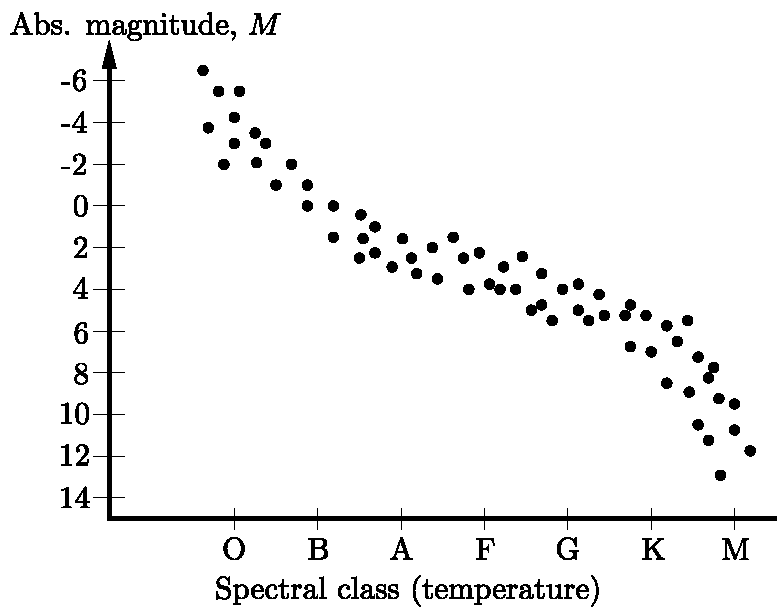
\includegraphics[scale=0.38]{media/fig_11-4a.pdf}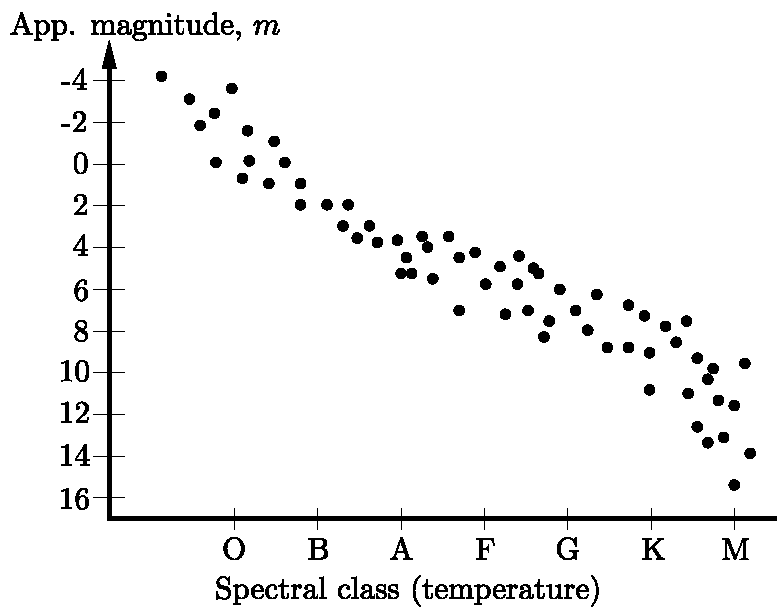
\includegraphics[scale=0.38]{media/fig_11-4b.pdf}}
\centerline{\includegraphics[scale=0.2]{media/fig_11-4comb.png}}
La oss velge ut en gitt temperatur, f.eks. den markert med A på x-aksen. Hvis vi ser på stjernene med denne temperaturen for hopen vår på figuren til høyre så ser vi at {\bf stjerner med denne temperaturen har en tilsynelatende størrelseklasse på omkring 4, enig?} Samtidig ser vi på diagrammet til venstre at {\bf stjerner med denne temperaturen skal ha en absolutt størrelseklasse på ca.2?} Dvs. stjerner i denne hopen med størrelseklasse 4 får størrelseklasse 2 (altså blir sterkere!) hvis de flyttes til 10 pc. \textcolor{red}{Det må vel bety at de er lenger unna enn 10 pc?}
\hyperlink{msfit19}{\pagebutton{Ja, det er jammen sant!}}
\end{frame}


\begin{frame}
\label{msfit19}
\lastpagebutton{msfit18}
%\centerline{\includegraphics[scale=0.38]{media/fig_11-4a.pdf}\includegraphics[scale=0.38]{media/fig_11-4b.pdf}}
\centerline{\includegraphics[scale=0.2]{media/fig_11-4comb.png}}
Tilbake til hovedspørsmålet:\\
 {\bf Kan du bruke disse to diagrammene samt formelen
\[
m-M=5\log{\frac{r}{10\mathrm{pc}}}
\]
til å finne avstanden til stjernehopen i diagrammet til høyre?} Er den ...\\

\hyperlink{feil_msfit19a}{\choicebutton{8pc}}\ \ \ \hyperlink{feil_msfit19a}{\choicebutton{10pc}}\ \ \ \hyperlink{feil_msfit19a}{\choicebutton{12pc}}\ \ \ \hyperlink{riktig_msfit19b}{\choicebutton{25pc}}\ \ \ \hyperlink{feil_msfit19a}{\choicebutton{50pc}}\ \ \ \hyperlink{feil_msfit19a}{\choicebutton{100pc}}\ \ \ 
\end{frame}


{
\setbeamercolor{background canvas}{bg=black}
\begin{frame}
\label{feil_msfit19a}
\lastpagebutton{msfit19}
\textcolor{yellow}{\Large Det ble nok galt! Hvorfor tar du ikke utgangspunkt i stjernene med temperatur A slik som vi gjorde på de forrige sidene? Vi vet jo at diagrammet har blitt skiftet opp/ned med en konstant størrelse (gå tilbake igjen hvis du er usikker på hvorfor), så da skulle vi få samme resultat uansett hvilken temperatur vi ser på. Da har du $m$ og $M$...}
\end{frame}
}

{
\setbeamercolor{background canvas}{bg=yellow}
\begin{frame}
\label{riktig_msfit19b}
\clastpagebutton{msfit19}
Det er helt riktig! Hvis vi ser på f.eks. temperaturen A så ser vi at diagrammet har blitt skiftet opp med $m-M=2$. Siden avstanden $r$ er omtrent den samme for alle stjerner så er jo dette skiftet fra $m$ til $M$ en konstant størrelse for alle stjernene i hopen (og dermed for alle temperaturer):
\[
m-M=5\log{\frac{r}{10\mathrm{pc}}}
\]
Prøv gjerne med en annen temperatur og du vil enda finne $m-M=2$. Det vi har gjort er å {\bf tilpasse} hovedserien fra HR-diagrammet med $m$ på y-aksen til hovedserien i HR-diagrammet med $M$ på y-aksen. Vi finner at hvis vi flytter hovedserien i HR-diagrammet for hopen med ukjent avstand med $m-M=2$ så vil de to diagrammene ligge nøyaktig på hverandre. Når vi har funnet det konstante skiftet $m-M$, så kan vi bare putte inn i formelen og finne avstanden. 
\hyperlink{msfit20}{\pagebutton{Neste side}}
\end{frame}
}


\begin{frame}
\label{msfit20}
\lastpagebutton{riktig_msfit19b}
Du har altså gjort en {\bf hovedserietilpasning} for å finne avstanden til stjernehopen. Prinsippet er jo at du kjenner hvordan fordelingene av luminositeter (absolutte størrelseklasser) som funksjon av temperatur (HR-diagram) {\bf skal} være for en slik hop. Og så ser du på fordelingen av mottatt fluks som funksjon av temperatur for stjernene i en hop med ukjent avstand. Siden du vet hvilke luminositeter disse stjernene egentlig har, så justerer du avstanden helt til du finner en avstand som gir det den målte mottatte fluksen gitt at du kjenner luminositeten. Dette var en annen måte å forklare hovedserietilpasning på.\\
\vspace*{0.4cm}
{\bf Har du lagt merke til at dette virkelig er en avstandsstige: vi måtte først ta det første steget og finne avstander til hoper med hjelp av parallakse. Kun etter at vi hadde avstanden til noen hoper, kunne vi lage HR-diagrammet med $M$ på y-aksen. Og med denne kunne vi nå finne avstanden til hoper så langt unna at parallakse ikke funker.}\\
\vspace*{0.4cm}
\textcolor{red}{Hvis du forstod hvordan hovedserietilpasning funker og prinsippet bak, {\bf gå videre til neste side.} Hvis ikke, ta en kikk på \href{https://www.uio.no/studier/emner/matnat/astro/AST2000/h20/undervisningsmateriell/interaktive-forelesningsnotater/3a/videoer/video3a_1.mp4}{denne videoen her}}.
\hyperlink{feil_msfit21}{\pagebutton{Neste side}}
\end{frame}


{
\setbeamercolor{background canvas}{bg=black}
\begin{frame}
\label{feil_msfit21}
\lastpagebutton{msfit20}
\centerline{\includegraphics[scale=0.09]{media/open_cluster_NGC265.jpg}}
\textcolor{yellow}{Tilbake til vår åpne hop NGC265 som ligger i den Store Magellanske Sky. Når vi gjør hovedserietilpasning til denne åpne hopa, så finner vi jo faktisk også ut omtrent hvor langt unna den Store Magellanske Sky ligger! Men hovedserietilpasning har begrenset rekkevidde. Vi klarer ikke å se enkeltstjerner i galaksehoper i galakser utenfor vårt eget nabolag av satelittgalakser. Dermed trenger vi andre metoder for å finne avstander til andre galakser.}
\hyperlink{feil_pause}{\pagebutton{Neste side}}
\end{frame}
}

{
\setbeamercolor{background canvas}{bg=black}
\begin{frame}
\label{feil_pause}
\hyperlink{feil_msfit21}{\pagebutton{\small Forrige side}}
\begin{columns}
\column{0.5\textwidth}
{\Huge\bf \centerline{\textcolor{yellow}{Kaffe?}}}
\vspace*{-0.9cm}
\centerline{\includegraphics[scale=0.45]{media/ladder_coffee.png}}
\column{0.5\textwidth}
{\Large \textcolor{yellow}{
Før vi begir oss ut på de mer svimlende avstandene, trenger vi litt kaffe. Det konseptuelt vanskligste i denne delen er over, resten er litt greiere.}}\\
\vspace*{0.5cm}
{\Large \textcolor{yellow}{
Ihvertfall 15 min pause...
}}\\
\vspace*{0.5cm}
\hyperlink{feil_nytema3}{\pagebutton{\small Klar for steget ut av vår galakse?}}
\end{columns}
\end{frame}
}

\renewcommand{\headline}{\small avstandsindikatorer}
{
\setbeamercolor{background canvas}{bg=black}
\begin{frame}
\label{feil_nytema3}
\begin{columns}
\column{0.5\textwidth}
\includegraphics[scale=0.4]{media/ladder3.png}
\hyperlink{feil_msfit21}{\pagebutton{\small Forrige side}}
\column{0.5\textwidth}
\textcolor{red}{\small Vi tar det tredje steget på avstandsstigen:}\vspace*{1cm}
\nytemaside{tf}
\vspace*{-0.5cm}\textcolor{red}{\small Omtrent hit (normalt 5-6 sider til) kommer jeg etter en dobbelttime fysisk forelesning. Du bør vurdere om du også vil vente med resten til imorgen? Eller er du frisk og opplagt og klar til resten allerede?}
\hyperlink{di1}{\pagebutton{La oss klatre videre!}}
\end{columns}
\end{frame}
}



\begin{frame}
\label{di1}
\lastpagebutton{feil_msfit21}\label{cepheider}
{\footnotesize
For å kunne måle avstander lenger utover i universet, trenger vi en av de aller viktigste metodene for avstandsmålinger: {\bf avstandsindikatorer}. Avstandsindikatorer er objekter som på en eller annen måte avslører egenskaper ved seg selv som gjør at de kan brukes til avstandsmålinger. Det er to typer:
\begin{itemize}
\item {\bf Standard-lyskilder} er objekter som på en eller annen måte avslører hvilken luminositet (og dermed hvilken absolutt størrelseklasse) de har. Hvis vi dermed kjenner absolutt størrelseklasse $M$, og så lenge vi kan observere objektet så vet vi den tilsynelatende størrelseklassen $m$, ja da kan vi finne avstanden ved hjelp av sammenhengen:
\[
m-M=5\log{\frac{r}{10\mathrm{pc}}}
\]
\item {\bf Standard-målestokker} er objekter som på en aller annen måte avslører hvor store de er, altså hva de fysiske dimensjonene er, f.eks. hvilken radius de har. Så lenge vi kan observere objektet, kan vi finne hvilken vinkelutstrekning $\theta$ de har på himmelen. Da kan vi bruke liten-vinkel-formel til å finne avstanden:
\[
r=\theta d
\]
der $r$ er fysisk radius til objektet, $\theta$ er den tilsvarende vinkelutstrekningen og $d$ er avstanden til objektet.
\end{itemize}
Det finnes mange slike avstandsindikatorer, \textcolor{red}{i AST2000 skal vi kun se på to slike, begge er standard-lyskilder: (1) Kefeidestjerner og (2) Supernovaeksplosjoner av type Ia. Vi begynner med Kefeidestjernene.}
}
\hyperlink{di2}{\pagebutton{Neste side}}
\end{frame}


\begin{frame}
\label{di2}
\lastpagebutton{di1}
\begin{block}{\bf Kefeider eller Kefeidestjerner (engelsk: Cepheids)...}
...er pulserende stjerner. Dette er aldrende stjerner som har begynt den sakte veien mot slutten av livsløpet sitt. Noen aldrende stjerner vil gå gjennom perioder der stjernen pulserer, dvs. at de endrer radiusen sin regelmessig, ofte med periode på noen dager. Noen av de første pulserende stjernene av denne typen som ble studert var stjernen $\delta$ Cephei i stjernebildet \href{https://snl.no/Kefeus}{Kefeus}, derav navnet.
\end{block}
Det som gjør Kefeidene spesielle er at pulsasjonsperioden sterkt avhenger av luminositeten til stjerna. Store massive stjerner med stor luminositet pulserer sakte, lette mindre massive stjerner (som har mindre luminositet) pulserer raskere. \textcolor{red}{Fra pulsasjonsperioden kan man dermed finne lumninositeten og derav den absolutte størrelseklassen} (som jo bare er luminositet målt i en spesiell enhet). Og med det kan vi som beskrevet tidligere finne avstanden.
\hyperlink{di2b}{\pagebutton{Neste side}}
\end{frame}



\begin{frame}
\label{di2b}
\lastpagebutton{di2}
Ved hjelp av målinger på Kefeider med {\bf kjent avstand}, har man funnet følgende sammenheng mellom pulsasjonsperiode $P_d$ i {\it dager} og absolutt størrelseklasse $M_V$. Merk at den absolutte størrelseklassen her har en indeks $V$ som står for visuell. Dvs. at størrelseklassen er basert på fluks i den visuelle delen av det elektromagnetiske spektret, dette skal vi straks se litt på, men vi snakker om en absolutt størrelseklasse (som er et mål på luminositet). {\bf Periode-Luminositets-relasjonen for Kefeider er (empirisk):}
\[
M_V=-2.81\log_{10}P_d-1.43
\]
\textcolor{red}{Merk igjen hvordan dette er en {\bf avstandsstige}. For å finne denne sammenhengen mellom luminositet og pulsasjonsperiode for Kefeider, trengte man først å kjenne avstanden til en rekke Kefeider ved hjelp av andre metoder som er de to første på stigen vår. Ved å kjenne avstandene til Kefeidene kunne man finne den absolutte størrelseklassen og dermed komme frem til denne relasjonen.} Som vi så benytter til å finne avstanden til Kefeider i ukjent avstand.
\hyperlink{di3}{\pagebutton{Neste side}}
\end{frame}


\begin{frame}
\label{di3}
\lastpagebutton{di2b}
Edwin Hubble var en av de første som prøvde å måle avstanden til nabogalaksen vår Andromeda. Han fant flere pulserende stjerner i den og brukte periode-luminositets-relasjonen til disse til å måle avstanden. Han fant at avstanden til Andromeda-galaksen er omkring en million lysår. Idag vet vi at den faktiske avstanden er to og en halv gang så stor. {\bf Hvordan fikk han så feil tall?} Man har i ettertid oppdaget at pulserende stjerner deler seg inn i 3 typer, hver med sin egen periode-luminositets-relasjonen. \textcolor{red}{Man må altså vite hvilken av disse 3 typene stjerne man har før man kan bruke den respektive periode-luminositets-relasjonen for å finne avstanden!}. {\bf De 3 typene er:}
\begin{itemize}
\item \textcolor{blue}{De klassiske Kefeidene} som vi akkurat snakket om. Fordelen med disse er at de er svært lyssterke og lett kan sees i fjerne galakser.
\item \textcolor{blue}{W Viriginies-stjerner} (først oppdaget i stjernebildet Jomfruen (Wirgo, derav navnet)). Disse er mer lyssvake en Kefeidene.
\item \textcolor{blue}{RR Lyrae-stjerner} (fra stjernebildet Lyra), svært lysvake stjerner som er vanskelig å se på stor avstand, men fordelen er at det er mange av disse.
\end{itemize}
{\small\bf I AST2000 skal vi konsentrere oss om de klassiske Kefeidene og periode-luminositets-relasjonen for disse.}\hyperlink{di4}{\pagebutton{\small Neste side}}
\end{frame}


\begin{frame}
\label{di4}
\lastpagebutton{di3}
La oss gå tilbake til periode-luminositets-relasjonen:
\[
M_V=-2.81\log_{10}P_d-1.43
\]
$M_V$ er absolutt størrelseklasse med {\bf Visuelt filter.} For å forklare dette med filtre, la oss for øyeblikket gå tilbake til {\it tilsyndelatende størrelseklasser}.  \textcolor{red}{Husker du definisjonen av tilsynelatende størrelseklasse?} Var det ikke
\[
m_1-m_2=-2.5\log{\frac{F_1}{F_2}}
\]
??? Her var $m_1$ og $m_2$ de tilsynelatende størrelseklassene til de to objektene og $F_1$ og $F_2$ var den tilsvarende mottatte fluksen fra disse to legemene. Hvis vi nå ønsker å rett og slett ha en formel for størrelseklassen $m$ til {\bf en} gitt stjerne hvis vi kjenner fluksen $F$ til denne stjerna, så trenger vi å introdusere et referanseobjekt med kjent størrelseklasse og kjent mottatt fluks (f.eks. stjernen Vega som har størrelseklasse $m=0$). Da finner vi relasjonen som vi ønsker oss:
\[
m=m_\mathrm{ref}-2.5\log{\frac{F}{F_\mathrm{ref}}}
\]
\hyperlink{di5}{\pagebutton{Neste side}}
\end{frame}

\begin{frame}
\label{di5}
\lastpagebutton{di4}
Men nå skulle vel vi snakke om {\bf absolutt} størrelseklasse? Ikke tilsynelatende? \textcolor{red}{OK, men det var jo bare a flytte objektet til en avstand av 10pc, var det ikke? Altså skal vi bruke mottatt fluks fra objektet, hvis dette objektet hadde befunnet seg i en avstand av 10pc.} Vi kaller $F(10\mathrm{pc})$ for mottatt fluks fra objektet hvis det blir flyttet til en avstand av 10pc. Da får vi for absolutt størrelseklasse at
\[
M=M^\mathrm{ref}-2.5\log{\frac{F(10\mathrm{pc})}{F^\mathrm{ref}(10\mathrm{pc})}}
\]
(denne kommer fra likningen på forrige side, etter at vi har flyttet objektene til avstand 10 pc, eller beregnet hvilken fluks {\it de ville hatt} i den avstanden, henger du med?)
Men uten å ha tenkt så mye over det før, så er jo $F$ her total fluks over alle mulige bølgelengder, fra radio til gammastråling. En slik total {\bf bolometrisk} fluks med tilhørende {\bf bolometrisk størrelseklasse} er vanskelig å måle. 
\hyperlink{di6}{\pagebutton{Neste side}}
\end{frame}

\begin{frame}
\label{di6}
\lastpagebutton{di5}
{\small
Når man måler fluksen fra et objekt så kan {\bf detektoren normalt kun måle fluks i et begrenset bølgelengdeområde.} Den fluksen som blir målt fra \textcolor{red}{en detektor som er sensitiv til synlig lys (og ikke andre bølgelender) gir oss ut en målt fluks $F_V$ (mens hvis du hadde observert absolutt alle bølgelengder, så hadde du målt fluks $F$).} Den fluksen vi måler med en detektor som er sensitiv til synlig lys er dermed en {\it filtrert fluks}:
\[
F_V=\int_0^\infty F(\lambda)S_V(\lambda)d\lambda
\]
Her er $S_V(\lambda)$ et {\bf filter} (bestemt av detektoren) som sier noe om hvor mye av hver bølgelengde som blir målt. $V$ betyr at dette filteret har en topp i den Visuelle delen av spektret, altså i vanlig synlig lys, og faller fort av. Mens $F(\lambda)$ er fluksen vi mottar for en gitt (hvilken som helst $\lambda$). {\bf Denne blir ganget med $S_V(\lambda)$. Effekten av detektoren er at den mottatte fluksen $F(\lambda)$ blir filtrert med $S_V(\lambda)$, dermed blir $F_V$ i praksis fluks målt kun med bølgelengder for synlig lys.} \textcolor{red}{Da får vi tilsvarende visuelle tilsynelatende og absolutte størreleklasser, $m_V$ og $M_V$.} Alle uttrykk som vi har utledet for størrelseklasser gjelder også for disse størrelseklassene med filtre, men $F$ må byttes med $F_V$. Vi har da
\[
M_V=M_V^\mathrm{ref}-2.5\log{\frac{F_V(10\mathrm{pc})}{F_V^\mathrm{ref}(10\mathrm{pc})}}
\]
}
\hyperlink{di7}{\pagebutton{Neste side}}
\end{frame}




\begin{frame}
\label{di7}
\lastpagebutton{di6}
Helt tilsvarende finnes det blå (B) og ultrafiolette (U) filtre med topper i de respektive bølgelgendeområder.
\begin{itemize}
\item V-filtret er et gaussisk filter med topp på $\lambda_0=550$nm og FWHM=89nm.
\item B-filtret er et gaussisk filter med topp på $\lambda_0=440$nm og FWHM=98nm.
\item U-filtret er et gaussisk filter med topp på $\lambda_0=365$nm og FWHM=68nm.
\end{itemize}
{\bf Dermed vil et og samme objekt kunne ha forskjellige størrelseklasser $m_V$, $m_B$ og $m_U$ avhengig av hvor mye fluks vi mottar fra dem i de forskjellige bølgelengdeområdene.} En blålig stjerne vil ha mindre størrelseklasse (altså være sterkere!) i $m_B$ enn i $m_V$. For Kefeider har man altså brukt observasjoner i den visuelle delen av spektret og slik har man da funnet periode-luminositetsrelasjonen for $M_V$.
\hyperlink{di7b}{\pagebutton{Neste side}}
\end{frame}

\begin{frame}
\label{di7b}
\lastpagebutton{di7}
{\bf Eksempel: Avsluttende eksamen fra 2009.}
\includegraphics[scale=0.35]{media/cepheide_kurve.png}\\
Kurven viser visuell tilsynelatende størrelseklasse $m_v$ for en Kefeidestjerne. Anslå avstanden til stjerna? Husk sammenhengen
\[
M_V=-2.81\log_{10}P_d-1.43\ \ \ \mathrm{og}\ \ \ m-M=5\log{\frac{r}{10\mathrm{pc}}}
\]
\hyperlink{feil_di7c}{\choicebutton{$14\mathrm{ly}$}}\ \ \ \ \hyperlink{feil_di7c}{\choicebutton{$26\mathrm{ly}$}}\ \ \ \ \hyperlink{feil_di7c}{\choicebutton{$84\mathrm{ly}$}}\ \ \ \ \hyperlink{riktig_di7d}{\choicebutton{$200\mathrm{ly}$}}\ \ \ \ \hyperlink{feil_di7c}{\choicebutton{$319\mathrm{ly}$}}
\end{frame}

{
\setbeamercolor{background canvas}{bg=black}
\begin{frame}
\label{feil_di7c}
\lastpagebutton{di7b}
\textcolor{yellow}{\Huge Det ble nok galt! Husker du at perioden $P_d$ skal være i {\bf dager}? Eller har du fått minustegnene riktig? Eller la du merke til at svaret var i {\bf lysår} og ikke i parsec? Hvis du ikke har gjor noen av disse feilene, ta en titt på \href{https://www.uio.no/studier/emner/matnat/astro/AST2000/h20/undervisningsmateriell/interaktive-forelesningsnotater/3a/videoer/video3a_2.mp4}{denne videoen} for å få noen tips.}
\end{frame}
}


{
\setbeamercolor{background canvas}{bg=yellow}
\begin{frame}
\label{riktig_di7d}
\clastpagebutton{di7b}
Helt riktig! På eksamen, pass på ikke å glemme at $P_d$ er i {\bf dager}!. Hvis du fikk dette til uten problemer, gå videre til neste side. Hvis du er litt usikker kan du se på \href{https://www.uio.no/studier/emner/matnat/astro/AST2000/h20/undervisningsmateriell/interaktive-forelesningsnotater/3a/videoer/video3a_2.mp4}{denne videoen}.
\hyperlink{di8}{\pagebutton{Neste side}}
\end{frame}
}




\begin{frame}
\label{di8}
\lastpagebutton{di7b}
{\bf Kefeider er svært lyssterke stjerner og kan sees i galakser så langt som 30Mpc unna! Det vil si at de kan brukes til å finne avstander til galakser som ligger millioner av lysår borte. Men for galakser som ligger enda lenger borte trenger vi standard-lyskilder som er enda mer lyssterke.} En slik standard-lyskilde kan være...
\begin{block}{\bf supernovaeksplosjoner}
Dette er kraftige eksplosjoner, så kraftig at når det har skjedd i vår egen Melkevei (skjer ca. en gang hvert 400. år) så har man iblant kunnet lese om natten i lyset fra supernovaen. En slik eksplosjon gir et ekstremt kraftig lys som varer i en dag eller to og er ofte klart synlig også om dagen. De deles opp i to typer:
\begin{itemize}
\item Supernova av type I er eksplosjoner hvor man ikke finner absorpsjonsliner fra Hydrogen i spektret. Disse deles videre opp i type Ia, Ib og Ic avhengig av hvilke andre absorpsjonsliner man finner.
\item Supernova av type II er eksplosjoner der man finner sterke absorpsjonsliner fra overganger i Hydrogenatomet.
\end{itemize}
\end{block}
\hyperlink{di9}{\pagebutton{Neste side}}
\end{frame}


\begin{frame}
\label{di9}
\lastpagebutton{di8}
Vi vet idag at
\begin{itemize}
\item ...supernovaer av type Ib, Ic og type II er såkalte kjernekollaps-supernovaer, altså stjerner som dør i en kraftig eksplosjon. Nøyaktiv hvordan og hvorfor kommer vi tilbake til om et par forelesninger.
\item ...supernovaer av type Ia er et annet fenomen, sannsynligvis oppstår disse kun i dobbeltstjernesystemer der en allerede død stjerne, en såkalt hvit dvergstjerne, suger til seg materiale fra naboen og til slutt når en kritisk massegrense og eksploderer.
\end{itemize}
Siden denne kritiske massegrensen alltid er den samme, så vil luminositeten, energien som frigjøres i eksplosjonen, også alltid være omtrent den samme. Supernovaer av type Ia er derfor meget gode {\bf standardlyskilder}.
\hyperlink{feil_di10}{\pagebutton{Neste side}}
\end{frame}


{
\setbeamercolor{background canvas}{bg=black}
\begin{frame}
\label{feil_di10}
\lastpagebutton{di9}
\begin{columns}
\column{0.5\textwidth}
\includegraphics[scale=0.1]{media/SNIa.jpg}
\textcolor{yellow}{\small Vi kommer til detaljene senere i del 3, men her er hovedlinjene: Når en stjerne med masse mindre enn ca. 8 solmasser dør, så kaster den av seg de ytre lagene sine litt om litt helt til vi står igjen med kjernen i stjerna som ofte er omtrentlig på størrelse med jorda. Den inneholder meget tett og varm {\bf elektron- degenerert gass}. Vi kaller det en {\bf hvit dvergstjerne.}}
\column{0.5\textwidth}
 \textcolor{yellow}{\small Hvis nabostjernen i dobbelt- stjernesystemet går i bane nær denne hvite dvergen vil gravitasjonsfeltet fra den hvite dvergen suge til seg materiale fra overflaten av nabostjerna. Litt om litt vil størrelsen på den hvite dvergen øke, det samme vil temperaturen og tettheten. På et tidspunkt når den hvite dvergen en masse på $1.4M_\odot$ som vi kaller {\bf Chandrasekhargrensen}. Med denne massen kan ikke degenerasjonstrykket i dvergen lenger stå imot gravitasjonen. Hele stjernen rives i biter i eksplosjonen som følger. Du kan se en \href{https://photojournal.jpl.nasa.gov/archive/PIA22352_SupernovaType1a_R3.mp4}{animasjon av prosessen her} (krever stor båndbredde).}
\hyperlink{feil_di11}{\pagebutton{Neste side}}\\
{\tiny\textcolor{yellow}{Bilde: NASA/JPL-Caltech}}
\end{columns}
\end{frame}
}



{
\setbeamercolor{background canvas}{bg=black}
\begin{frame}
\label{feil_di11}
\lastpagebutton{feil_di10}
\begin{columns}
\column{0.5\textwidth}
\includegraphics[scale=0.1]{media/SNIa.jpg}
\textcolor{yellow}{\footnotesize Massen av stjerna som eksploderer er dermed alltid omkring $1.4M_\odot$, og energien som frigjøres er alltid omtrent den samme. Ved å se på eksplosjoner i galakser der man har observert Kefeider (og som man derfor kjenner avstanden til), har man kunnet måle luminositeten (og dermed den absolutte størrelseklassen $M$) til disse eksplosjonene. Denne er $M_V\approx M_B\approx19.3$ med et avvik på opp til 0.3.}
\column{0.5\textwidth}
\textcolor{yellow}{\footnotesize  Ved nøye observasjoner av mange slike supernovaer i galakser med kjent avstand kan man nå beregne også dette lille avviket ved å bruke formen på lyskurven. Absolutt størrelseklasse til en slik eksplosjon kan dermed bestemmes ganske nøyaktig som gjør disse til gode standardlyskilder for å finne avstanden til galaksen som supernovaeksplosjonen skjer i ved:
\[
m-M=5\log{\frac{r}{10\mathrm{pc}}}
\]
Supernovaer av type Ia er svært lyssterke og kan observeres i galakser som er over 1000Mpc unna. De kan altså brukes til å bestemme avstanden til svært fjerne og lyssvake galakser, milliarder av lysår borte. {\bf MEN, for å kunne bruke metoden må vi være så heldig at det faktisk skjer en slik supernova der!} Det er den store ulempen med denne metoden.
} \hyperlink{feil_nytema4}{\pagebutton{Neste side}}
\end{columns}
\end{frame}
}


\renewcommand{\headline}{\small Tully-Fisher-relasjonen}
{
\setbeamercolor{background canvas}{bg=black}
\begin{frame}
\label{feil_nytema4}
\begin{columns}
\column{0.5\textwidth}
\includegraphics[scale=0.4]{media/ladder4.png}
\hyperlink{feil_di11}{\pagebutton{\small Forrige side}}
\column{0.5\textwidth}
\textcolor{red}{\small Vi tar det fjerde steget på avstandsstigen:}\vspace*{1cm}
\nytemaside{hl}
\hyperlink{tf1}{\pagebutton{Tulle...hvafforno'?}}
\end{columns}
\end{frame}
}



\begin{frame}
\label{tf1}
\lastpagebutton{feil_di11}\label{tf}
{\bf Tully-Fisher-relasjonen er en sammenheng mellom bredden av 21cm-emisjonslinja fra en galakse og absolutt størrelseklasse (luminositet) til denne galaksen.} Hvis vi fra bredden av 21cm-linja kan finne luminositeten til galaksen, ja da har vi egentlig nok en standard-lyskilde, dvs. et objekt (en galakse) som forteller hva luminositeten her. Og vi kan bruke samme likning som tidligere for å finne avstanden.\\
\vspace*{1cm}
{\bf Men hva var nå 21cm-linja igjen?} Husker du fra del 1D at nøytralt hydrogen sender ut stråling med bølgelengde 21cm fra en såkalt spin-flip? (hvis ikke, ta en \href{https://www.uio.no/studier/emner/matnat/astro/AST2000/h20/undervisningsmateriell/lecture\_notes/part1d.pdf}{kikk tilbake igjen} nå). \textcolor{red}{En spiralgalakse inneholder mange skyer av nøytralt hydrogen. Disse går i baner rundt galaksesenteret på samme måte som stjernene i mange forskjellige avstander fra galaksesenteret.}\\
\vspace*{0.5cm}
{\Large Men hvordan kan bredden til 21cm linja gi oss luminositeten til galaksen?}
\hyperlink{tf2}{\pagebutton{Neste side}}
\end{frame}



\begin{frame}
\label{tf2}
\lastpagebutton{tf1}
{\huge På de neste sidene skal du få gjøre litt detektivarbeid. Du skal se rett og slett se hvor mange tips du trenger før du innser {\bf hvorfor} det er en sammenheng mellom bredden av 21cm-linja og luminositeten til galaksen. {\bf MERK at det ikke er meningen at du skal finne denne sammenhengen, den er komplisert, men du skal innse hvorfor det finnes en sammenheng her.}}
\textcolor{red}{Første forsøk kommer nå: klarer du å se {\bf hvorfor} det er en slik sammenheng uten noe tips? Tegn galaksen med hydrogenskyene i bane, det kan være til hjelp.}
\hyperlink{tf3}{\pagebutton{Tenk deg godt om før du går til første tips!}}
\end{frame}

\begin{frame}
\label{tf3}
\lastpagebutton{tf2}
\begin{alertblock}{Tips 1:}
Emisjonslinjen på 21cm fra en galakse har en meget spesiell form. Ta en kikk på \href{https://www.uio.no/studier/emner/matnat/astro/AST2000/h20/undervisningsmateriell/interaktive-forelesningsnotater/3a/videoer/video3a_3.mp4}{denne videoen} for å se formen på linja. Kan du tenke deg hvorfor linja har denne formen? Og hjelper det deg til å forstå hvorfor vi har en sammenheng mellom bredden av 21cm-linja og luminositeten til galaksen?
\end{alertblock}
\hyperlink{tf4}{\pagebutton{Tenk deg godt om før du går til andre tips!}}
\end{frame}

\begin{frame}
\label{tf4}
\lastpagebutton{tf3}
\begin{alertblock}{Tips 2:}
{\Huge Dopplereffekten! Kom du på sporet nå?}
\end{alertblock}
\hyperlink{tf5}{\pagebutton{Tenk deg godt om før du går til tredje tips!}}
\end{frame}

\begin{frame}
\label{tf5}
\lastpagebutton{tf4}
\begin{alertblock}{Tips 3:}
Forrige tips fortalte deg at Dopplereffekten gir opphave til den spesielle formen på linja. I \href{https://www.uio.no/studier/emner/matnat/astro/AST2000/h20/undervisningsmateriell/interaktive-forelesningsnotater/3a/videoer/video3a_4.mp4}{denne videoen} får du se hvordan! {\bf MEN det som ikke kommer frem i videoen er hvorfor de to toppene på siden er høyere enn i sentrum av linja.} Akkurat dette er nøkkelen til hvorfor vi har en sammenheng mellom bredden av 21cm-linja og luminositeten til galaksen. Ser du det nå?
\end{alertblock}
\hyperlink{tf6}{\pagebutton{Tenk deg godt om før du går til fjerde tips!}}
\end{frame}

\begin{frame}
\label{tf6}
\lastpagebutton{tf5}
\begin{alertblock}{Tips 4:}
{\Huge Mørk materie og galaktiske rotasjonskurver! Ser du nå hvorfor de to toppene på siden er høyere enn i sentrum av linja?}
\end{alertblock}
\hyperlink{tf7}{\pagebutton{Tenk deg godt om før du går til femte tips!}}
\end{frame}

\begin{frame}
\label{tf7}
\lastpagebutton{tf6}
\begin{alertblock}{Tips 5:}
I \href{https://www.uio.no/studier/emner/matnat/astro/AST2000/h20/undervisningsmateriell/interaktive-forelesningsnotater/3a/videoer/video3a_5.mp4}{denne videoen} får du se hvorfor vi har to topper. Vi vet altså at rotasjonskurven til galaksen flater ut og at alle hydrogenskyer i de ytre delene av galaksen har omtrent samme banehastighet og dermed omtrengt samme Dopplereffekt. Men hva avjør hvor langt $\Delta\lambda$ fra sentrum av linja denne toppen befinner seg? Ser du nå opphavet til sammenhengen?
\end{alertblock}
\hyperlink{tf8}{\pagebutton{Tenk deg godt om før du går til sjette tips!}}
\end{frame}

\begin{frame}
\label{tf8}
\lastpagebutton{tf7}
\begin{alertblock}{Tips 6:}
Fra Dopplereffekten har vi at $\Delta\lambda=\lambda_0\frac{v}{c}$. Det er altså banehastigheten $v$ til gass-skyene ytterst i galaksen som avgjør hvor langt ut $\Delta\lambda$ fra sentrum $\lambda_0$ av 21cm-linja at disse toppene befinner seg. Det er dermed også disse som avgjør bredden til linja. Men hva avhenger denne hastigheten $v$ av?
\end{alertblock}
\hyperlink{tf9}{\pagebutton{Tenk deg godt om før du går til syvende tips!}}
\end{frame}


\begin{frame}
\label{tf9}
\lastpagebutton{tf8}
\begin{alertblock}{Tips 7:}
Fra Keplers lover så må det vel være massen til galaksen som avgjør banehastigheten. Nå er vel omkring 85\% av denne massen mørk materie....Kom du litt nærmere løsningen på gåten nå?
\end{alertblock}
\hyperlink{tf10}{\pagebutton{Tenk deg godt om før du går til åttende tips!}}
\end{frame}

\begin{frame}
\label{tf10}
\lastpagebutton{tf9}
\begin{alertblock}{Tips 8:}
Høy banehastighet for de ytterste gass-skyene betyr høy galaksemasse, altså mye mørk materie. Men omkring 15\% av denne materien er jo også lysende materie i form av stjerner. Altså jo høyere hastighet, jo mer lysende materie og stjerner har vi også. Nå ser du det kanskje?
\end{alertblock}
\hyperlink{tf11}{\pagebutton{Tenk deg godt om før du går til løsningen!}}
\end{frame}



\begin{frame}
\label{tf11}
\lastpagebutton{tf10}
\begin{alertblock}{Løsningen på mysteriet}
Jo høyere hastighet på gass-skyene i de ytre delene av galaksen, jo høyere forskyvning av toppen i 21cm-linja, og dermed jo bredere 21cm-linje. Høyere hastighet betyr større masse, både mørk og lysende. Jo flere stjerner, jo større total luminositet på galaksen. Hvis du ikke helt henger med enda, ta en kikk på oppsummeringen i \href{https://www.uio.no/studier/emner/matnat/astro/AST2000/h20/undervisningsmateriell/interaktive-forelesningsnotater/3a/videoer/video3a_6.mp4}{denne videoen}
\end{alertblock}
Sammenhengen mellom bredden av linja og absolutt størrelseklasse er mest presis i blått lys og er dermed gitt ved absolutt størrelseklasse med blått filter:
\[
M_B=C_1+\log{v_\mathrm{max}}+C_2
\]
der $v_\mathrm{max}$ er Dopplerhastigheten som tilsvarer de to toppene i linja mens konstantene $C_1$ og $C_2$ avhenger av galaksetypen.
\hyperlink{tf12}{\pagebutton{Neste side}}
\end{frame}

\begin{frame}
\label{tf12}
\lastpagebutton{tf11}
{\Large Vi kan observere 21cm-linja til galakser i avstander opp til omkring 100Mpc. Denne metoden overlapper altså med både galakser der man kan se Kefeider og der man kan bruke supernova av type Ia, MEN fordelen med Tully-Fisher fremfor supernovaer er at Tully-Fisher alltid kan brukes, mens for supernovaer må man være heldig at det faktisk går av en supernova i en galakse. Det er i tillegg veldig viktig med overlappende metoder slik at de kan kontrolleres mot hverandre.}
\hyperlink{feil_nytema5}{\pagebutton{Neste side}}
\end{frame}




\renewcommand{\headline}{\small Hubbles lov}
{
\setbeamercolor{background canvas}{bg=black}
\begin{frame}
\label{feil_nytema5}
\begin{columns}
\column{0.5\textwidth}
\includegraphics[scale=0.4]{media/ladder5.png}
\hyperlink{tf12}{\pagebutton{\small Forrige side}}
\column{0.5\textwidth}
\textcolor{red}{\small Vi tar det siste steget på avstandsstigen:}\vspace*{1cm}
\nytemaside{0}
\hyperlink{hl1}{\pagebutton{\footnotesize Ut til det observerbare universets ytterkanter}}
\end{columns}
\end{frame}
}




\begin{frame}
\label{hl1}
\lastpagebutton{tf12}\label{hl}
Vi skal bare såvidt komme innom Hubbles lov i dette kurset. Edwin Hubble oppdaget på 1920-tallet at alle fjerne galakser hadde en rødforskyvning. Dvs. at de alle hadde en hastighet bort fra oss. Og ikke bare det, {\bf jo lenger borte galaksen var, jo større var rødforskyvningen, altså jo større hastighet hadde galaksen bort fra oss.} Dette formulerte han i Hubbles lov:
\[
v=H_0r
\]
hvor $v$ er hastigheten som galaksen fjerner seg fra oss med, $r$ er avstanden til galaksen og $H_0$ er Hubblekonstanten som er på ca. $H_0=71\mathrm{km}/\mathrm{s}/\mathrm{Mpc}$. Enhetene til konstanten kan vi tolke slik: for hver $Mpc$-avstand som galaksen har til oss, så øker hastigheten i forhold til oss med $71\mathrm{km}/\mathrm{s}$. \textcolor{red}{Ved å måle rødforskyvningen til spektrallinjer i en galakse og dermed finne hastigheten via Dopplereffekten kan man dermed finne avstanden ved Hubbles lov!}. Så lenge man kan observere en galakse vil man som regel klare å finne minst en spektrallinje som man kan måle rødforskyvning på. {\bf Dermed kan Hubbles lov brukes til å måle avstander helt ut til de aller fjerneste objektene som vi kan observere.}
\hyperlink{hl2}{\pagebutton{Neste side}}
\end{frame}



\begin{frame}
\label{hl2}
\lastpagebutton{hl1}
{\small
Hubbles lov er et resultat av {\bf universets ekspansjon}. Fra Einsteins generelle relativitetsteori kan man vise at målestokkene i universet utvider seg med tiden. Resultatet av dette er Hubbles lov. Den samme effekten ville blitt observert fra en hvilken som helst galakse i universet. {\bf Alle vil oppleve at alle fjerne galakser fjerner seg fra dem.} Hastigheten som måles med Dopplereffekten i dette tilfelle er ikke en vanlig hastighet men heller {\bf et mål på hvor fort rommet mellom oss og den fjerne galaksen utvider seg}.\\
\vspace*{1cm}
Man pleier å måle rødforskyvingen med en parameter $z$
\[
z=\frac{\Delta\lambda}{\lambda}
\]
Jo høyere $z$, jo større rødforskyvning og jo lenger ut i universet ligger objektene. Galakser på veldig stor avstand og dermed med veldig høy rødforskyvning $z$ vil få en rødlig farge da toppen av stråling fra galaksen har blitt skøvet ut i den røde delen av spektret. Noen ekstremt fjerne objekter kan til og med få strålingen forskøvet ut av den synlige delen av spektret slik at de kun kan observeres med infrarøde detektorer.
}
\hyperlink{oppsummering}{\pagebutton{Neste side}}
\end{frame}










\begin{frame}
\label{oppsummering}
\hyperlink{hl2}{\pagebutton{\small Forrige side}}\href{https://nettskjema.no/a/165595}{\Changey[1][yellow]{2} \Changey[1][yellow]{-2}}
Gratulerer, del 3A er overstått. Du bør nå:
\begin{itemize}
\item kjenne hovedmetodene for å måle avstander i universet
\item kunne måle avstander med parallaksemetoden
\item kunne måle avstander med hovedserietilpasning
\item kunne bruke Kefeidestjerner til å måle avstander
\item kunne bruke supernovaer av type Ia til å måle avstander
\item kunne forklare Tully-Fisher-relasjonen og bakgrunnen for denne
\item kunne bruke Hubbles lov til å måle avstander i universet
\end{itemize}
\textcolor{red}{Flott hvis du nå kan klikke på smilefjesene over og fortelle hva du synes om dette interaktive forelesningsnotatet. Hva var bra og nøyaktig hva kan forbedres? All ris og ros mottaes med takk!}
{\bf Det anbefales nå at du sjekker \href{https://www.uio.no/studier/emner/matnat/astro/AST2000/h21/undervisningsmateriell/kortsvarsoppgaver/del3a.pdf}{kortsvarsoppgavene} til del 3A for å kontrollere at du har forstått stoffet. Kan du svare på disse, blir det lettere å bruke kunnskapen din i oppgavene/prosjektet. Noen av disse kommer på eksamen.}
\end{frame}



\end{document}
